% ============================================================================
% gtfs-ingest -- The whole workflow (companion to docs/guide/pipeline-guide.md)
%
% Compile from presentations/ (figures are read from ../docs/figures/):
%     latexmk -pdf workflow.tex
%
% Only standard packages: beamer, tikz, listings, lmodern, xcolor, graphicx,
% tabularx. Regenerate the charts first with:
%     python docs/figures/make_figures.py --run outputs/out_mibici_v12 \
%         --before outputs/out_mibici_v9
% Every number comes from the run outputs/out_mibici_v12.
% ============================================================================
\documentclass[aspectratio=169,10pt]{beamer}

\usepackage[utf8]{inputenc}
\usepackage[T1]{fontenc}
\usepackage{lmodern}
\usepackage{microtype}
% keep "--" as two hyphens in code (CLI flags)
\DisableLigatures[-]{encoding = T1, family = tt*}
\usepackage{graphicx}
\usepackage{tabularx}
\usepackage{listings}
\usepackage{tikz}
\usetikzlibrary{positioning, arrows.meta, calc, shapes.geometric, fit, backgrounds}

\graphicspath{{../docs/figures/}}

% ---------------------------------------------------------------------------
% Palette -- identical to the chart palette in docs/figures/make_figures.py,
% so the embedded charts sit seamlessly on the slides.
% ---------------------------------------------------------------------------
\definecolor{cSurface}{HTML}{FCFCFB}
\definecolor{cInk}{HTML}{0B0B0B}
\definecolor{cInkTwo}{HTML}{52514E}
\definecolor{cMuted}{HTML}{898781}
\definecolor{cGrid}{HTML}{E1E0D9}
\definecolor{cBase}{HTML}{C3C2B7}
\definecolor{cContext}{HTML}{D6D5CE}
\definecolor{cCode}{HTML}{F1F0EC}
\definecolor{cBlue}{HTML}{2A78D6}
\definecolor{cOrange}{HTML}{EB6834}
\definecolor{cAqua}{HTML}{1BAF7A}
\definecolor{cYellow}{HTML}{EDA100}
\definecolor{cViolet}{HTML}{4A3AA7}
\definecolor{cRampLight}{HTML}{86B6EF}
\definecolor{cRampDark}{HTML}{0D366B}
% one hue per phase
\colorlet{cPOne}{cBlue}
\colorlet{cPTwo}{cAqua}
\colorlet{cPThree}{cOrange}
\colorlet{cPFour}{cViolet}
\definecolor{cRed}{HTML}{C8322B}
% toy model: one colour per route
\colorlet{cLone}{cRampDark}
\colorlet{cLtwo}{cRampLight}
\colorlet{cRten}{cOrange}
\colorlet{cRtwenty}{cYellow}

% ---------------------------------------------------------------------------
% Beamer look: quiet, ink-on-surface, one accent per phase
% ---------------------------------------------------------------------------
\usetheme{default}
\setbeamertemplate{navigation symbols}{}
\setbeamercolor{background canvas}{bg=cSurface}
\setbeamercolor{normal text}{fg=cInk}
\setbeamercolor{structure}{fg=cBlue}
\setbeamercolor{frametitle}{fg=cInk,bg=cSurface}
\setbeamercolor{title}{fg=cInk}
\setbeamercolor{subtitle}{fg=cInkTwo}
\setbeamercolor{item}{fg=cBlue}
\setbeamercolor{block title}{fg=cInk,bg=cGrid}
\setbeamercolor{block body}{fg=cInk,bg=cCode}
\setbeamercolor{block title alerted}{fg=white,bg=cOrange}
\setbeamercolor{block body alerted}{fg=cInk,bg=cOrange!8}
\setbeamercolor{block title example}{fg=white,bg=cAqua}
\setbeamercolor{block body example}{fg=cInk,bg=cAqua!8}
\setbeamerfont{frametitle}{series=\bfseries,size=\Large}
\setbeamerfont{title}{series=\bfseries,size=\LARGE}
\setbeamertemplate{itemize items}{\raisebox{0.15ex}{\tikz\fill[cBlue] (0,0) circle (0.45ex);}}
\setbeamertemplate{itemize subitem}{\raisebox{0.2ex}{\tikz\fill[cMuted] (0,0) circle (0.35ex);}}
\setbeamertemplate{blocks}[rounded][shadow=false]

\setbeamertemplate{frametitle}{%
  \vskip0.25cm%
  \usebeamerfont{frametitle}\usebeamercolor[fg]{frametitle}\insertframetitle%
  \ifx\insertframesubtitle\empty\else%
    \par\vskip2pt{\normalsize\color{cInkTwo}\mdseries\insertframesubtitle}%
  \fi%
  \vskip0.1cm%
}
\setbeamertemplate{footline}{%
  \hbox to \paperwidth{%
    \hskip0.6cm{\tiny\color{cMuted}gtfs-ingest \,$\cdot$\, The workflow%
      \ifx\insertsection\empty\else\,$\cdot$\, \insertsection\fi}%
    \hfill{\tiny\color{cMuted}\insertframenumber\,/\,\inserttotalframenumber}\hskip0.6cm}%
  \vskip0.3cm}

% ---------------------------------------------------------------------------
% Helpers
% ---------------------------------------------------------------------------
\newcommand{\code}[1]{\texttt{\detokenize{#1}}}
\newcommand{\muted}[1]{{\color{cInkTwo}#1}}
\newcommand{\step}[2]{% phase colour, step number -> small coloured badge
  {\setlength{\fboxsep}{2pt}\colorbox{#1}{\scriptsize\bfseries\color{white}STEP #2}}\hspace{0.4em}}

\lstdefinestyle{algo}{
  basicstyle=\ttfamily\scriptsize\color{cInk},
  backgroundcolor=\color{cCode},
  frame=none, framesep=0pt, xleftmargin=6pt, xrightmargin=6pt,
  aboveskip=4pt, belowskip=4pt,
  columns=fullflexible, keepspaces=true, showstringspaces=false,
  commentstyle=\color{cMuted}\itshape,
  keywordstyle=\color{cBlue}\bfseries,
  morekeywords={for,each,if,else,in,emit,drop,sort,by,group,and,or,not,return,while},
  morecomment=[l]{\#},
}
\lstdefinestyle{sql}{
  style=algo, language=SQL, morecomment=[l]{--},
  morekeywords={LATERAL,ST_DWithin,ST_Distance,ST_Transform,ST_MakePoint,ST_SetSRID,
    ST_Buffer,ST_ConvexHull,ST_Collect,ST_Intersects,COALESCE,NULLIF,RETURNING},
}

\tikzset{
  box/.style={draw=#1, fill=#1!9, rounded corners=3pt, align=center, font=\scriptsize,
              inner sep=4pt, text=cInk, line width=0.7pt},
  box/.default=cInkTwo,
  arr/.style={-{Stealth[length=2.2mm,width=1.8mm]}, line width=0.8pt, color=cInkTwo},
  darr/.style={arr, dashed},
  db/.style={cylinder, shape border rotate=90, aspect=0.22, draw=cInkTwo, fill=cContext!45,
             font=\scriptsize, align=center, minimum width=1.9cm, minimum height=1.0cm,
             line width=0.7pt, text=cInk},
  dec/.style={diamond, aspect=2.4, draw=#1, fill=#1!7, font=\tiny, align=center,
              inner sep=0.5pt, text=cInk, line width=0.7pt},
  dec/.default=cInkTwo,
  lbl/.style={font=\tiny, text=cInkTwo},
  yes/.style={font=\tiny\bfseries, text=cAqua!70!black, fill=cSurface, inner sep=1pt},
  no/.style={font=\tiny\bfseries, text=cOrange!80!black, fill=cSurface, inner sep=1pt},
  stop/.style={circle, fill=#1, draw=cSurface, line width=1pt, inner sep=2.6pt},
  stop/.default=cInkTwo,
  st/.style={box=#1, rounded corners=8pt, text width=2.2cm, minimum height=0.8cm},
  nd/.style={circle, draw=#1, fill=#1!12, line width=0.8pt, minimum size=1.15cm, font=\scriptsize\bfseries},
  tbl/.style={draw=#1, fill=cSurface, line width=0.8pt, rounded corners=3pt, anchor=north,
              text width=3.5cm, align=left, font=\tiny\ttfamily, inner sep=4pt},
  head/.style={fill=#1, text=white, font=\scriptsize\bfseries, rounded corners=3pt, anchor=south,
               minimum width=3.5cm+8pt, inner sep=3pt},
}

\newcommand{\cmark}{{\color{cAqua}\ensuremath{\checkmark}}}
\newcommand{\xmark}{{\color{cMuted}\ensuremath{\times}}}

% Toy model (schematic positions, not to scale; real distances are labelled)
\tikzset{
  stRail/.style={circle, fill=cBlue, draw=cSurface, line width=0.8pt, minimum size=8pt, inner sep=0pt},
  stBus/.style={rectangle, fill=cOrange, draw=cSurface, line width=0.8pt, minimum size=7.5pt, inner sep=0pt},
  stBike/.style={diamond, fill=cAqua, draw=cSurface, line width=0.8pt, minimum size=9.5pt, inner sep=0pt},
  unlinked/.style={fill=cSurface, draw=#1, line width=1.2pt},
  etq/.style={font=\scriptsize\bfseries, text=cInk, inner sep=1.5pt},
  tmin/.style={font=\tiny, fill=cSurface, inner sep=0.8pt, text=cInk},
  dist/.style={font=\tiny\itshape, text=cInkTwo, fill=cSurface, inner sep=0.8pt},
  ride/.style={-{Stealth[length=2.2mm,width=1.9mm]}, line width=1.4pt, color=#1},
  routeline/.style={line width=2.6pt, color=#1, opacity=0.3, line cap=round},
  walkarc/.style={densely dashed, line width=1.1pt, color=cInkTwo},
  samest/.style={double=cSurface, double distance=1.3pt, line width=0.7pt, color=cViolet},
  pathhl/.style={line width=6pt, color=cAqua, opacity=0.28, line cap=round, line join=round},
}
\newcommand{\toyCoords}{%
  \coordinate (A1) at (60,320);  \coordinate (A2) at (250,320);
  \coordinate (A3) at (480,320); \coordinate (A4) at (720,320);
  \coordinate (A5) at (800,390); \coordinate (A6) at (800,570);
  \coordinate (B1) at (300,60);  \coordinate (B2) at (300,265);
  \coordinate (B3) at (300,570); \coordinate (B4) at (500,570);
  \coordinate (B5) at (690,570);
  \coordinate (M1) at (60,430);  \coordinate (M2) at (560,110);}
\newcommand{\toyLines}{%
  \draw[routeline=cLone] (A1) -- (A4);
  \draw[routeline=cLtwo] (A5) -- (A6);
  \draw[routeline=cRten] (B1) -- (B3);
  \draw[routeline=cRtwenty] (B3) -- (B5);}
\newcommand{\toyStops}{%
  \node[stRail, label={[etq]below left:A1}] (nA1) at (A1) {};
  \node[stRail, label={[etq]above left:A2}] (nA2) at (A2) {};
  \node[stRail, label={[etq]above:A3}] (nA3) at (A3) {};
  \node[stRail, label={[etq]above:A4}] (nA4) at (A4) {};
  \node[stRail, label={[etq]right:A5}] (nA5) at (A5) {};
  \node[stRail, label={[etq]right:A6}] (nA6) at (A6) {};
  \node[stBus, label={[etq]right:B1}] (nB1) at (B1) {};
  \node[stBus, label={[etq]below right:B2}] (nB2) at (B2) {};
  \node[stBus, label={[etq]above:B3}] (nB3) at (B3) {};
  \node[stBus, label={[etq]above:B4}] (nB4) at (B4) {};
  \node[stBus, label={[etq]above:B5}] (nB5) at (B5) {};
  \node[stBike, label={[etq]left:M1}] (nM1) at (M1) {};
  \node[stBike, label={[etq]below:M2}] (nM2) at (M2) {};}
\newcommand{\toyRides}{%
  \draw[ride=cLone] (nA1) -- node[tmin, below] {2.0} (nA2);
  \draw[ride=cLone] (nA2) -- node[tmin, below, pos=0.3] {2.0} (nA3);
  \draw[ride=cLone] (nA3) -- node[tmin, below] {2.0} (nA4);
  \draw[ride=cLtwo] (nA5) -- node[tmin, left] {1.5} (nA6);
  \draw[ride=cRten] (nB1) -- node[tmin, left] {3.0} (nB2);
  \draw[ride=cRten] (nB2) -- node[tmin, left, pos=0.6] {3.5} (nB3);
  \draw[ride=cRtwenty] (nB3) -- node[tmin, below] {3.0} (nB4);
  \draw[ride=cRtwenty] (nB4) -- node[tmin, below] {2.5} (nB5);}
\newcommand{\toyDistances}{%
  \node[dist, right] at ($(A1)!0.5!(M1)$) {20 m};
  \node[dist] at (215,270) {0 m};
  \node[dist, below right] at ($(A4)!0.5!(A5)$) {28 m};
  \node[dist, below] at ($(A6)!0.5!(B5)+(0,-10)$) {71 m};}
\newcommand{\toyStopLegend}{%
  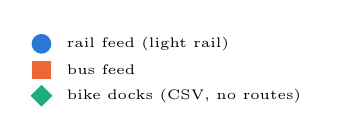
\begin{tikzpicture}[font=\tiny, x=1cm, y=1cm]
    \node[stRail] at (0,0) {};      \node[anchor=west] at (0.2,0) {rail feed (light rail)};
    \node[stBus] at (0,-0.33) {};   \node[anchor=west] at (0.2,-0.33) {bus feed};
    \node[stBike] at (0,-0.66) {};  \node[anchor=west] at (0.2,-0.66) {bike docks (CSV, no routes)};
  \end{tikzpicture}}
\newcommand{\toyArcLegend}{%
  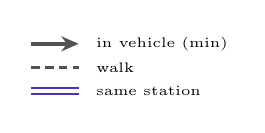
\begin{tikzpicture}[font=\tiny, x=1cm, y=1cm]
    \draw[ride=cInkTwo] (0,0) -- (0.6,0);   \node[anchor=west] at (0.7,0) {in vehicle (min)};
    \draw[walkarc] (0,-0.3) -- (0.6,-0.3);  \node[anchor=west] at (0.7,-0.3) {walk};
    \draw[samest] (0,-0.6) -- (0.6,-0.6);   \node[anchor=west] at (0.7,-0.6) {same station};
  \end{tikzpicture}}
\newcommand{\toyRouteLegend}{%
  
\begin{tikzpicture}[font=\tiny, x=1cm, y=1cm]
    \draw[line width=2pt, cLone] (0,0) -- (0.45,0);        \node[anchor=west] at (0.5,0) {L1};
    \draw[line width=2pt, cLtwo] (1.0,0) -- (1.45,0);      \node[anchor=west] at (1.5,0) {L2};
    \draw[line width=2pt, cRten] (2.0,0) -- (2.45,0);      \node[anchor=west] at (2.5,0) {R10};
    \draw[line width=2pt, cRtwenty] (3.1,0) -- (3.55,0);   \node[anchor=west] at (3.6,0) {R20};
  \end{tikzpicture}}

% Big number tile: value, label, accent
\newcommand{\stat}[3]{%
  \tikz\node[draw=#3, fill=#3!8, line width=0.8pt, rounded corners=4pt, minimum width=3.3cm,
             minimum height=1.5cm, align=center, inner sep=3pt]
    {{\LARGE\bfseries\color{cInk}#1}\\[3pt]{\scriptsize\color{cInkTwo}#2}};}

% Section divider: phase name, colour, subtitle, step list
\newcommand{\divider}[4]{%
  \begin{frame}[plain]
    \begin{tikzpicture}[remember picture, overlay]
      \fill[#2] (current page.north west) rectangle ([xshift=0.45cm]current page.south west);
      \node[anchor=west, font=\fontsize{30}{34}\selectfont\bfseries, text=cInk]
        at ([xshift=1.4cm, yshift=1.2cm]current page.west) {#1};
      \node[anchor=west, font=\large, text=cInkTwo]
        at ([xshift=1.42cm, yshift=0.15cm]current page.west) {#3};
      \node[anchor=north west, font=\small, text=cInk, align=left, text width=12cm]
        at ([xshift=1.42cm, yshift=-0.5cm]current page.west) {#4};
    \end{tikzpicture}
  \end{frame}}

% Severity badge for the validation table
\newcommand{\sevbadge}[2]{\tikz[baseline=(s.base)]\node[fill=#1,text=white,rounded corners=1.5pt,
  inner sep=1.6pt,font=\tiny\bfseries](s){\strut #2};}
\newcommand{\sevE}{\sevbadge{cOrange}{ERROR}}
\newcommand{\sevW}{\sevbadge{cYellow}{WARN}}
\newcommand{\sevI}{\sevbadge{cMuted}{INFO}}
% Data-model table: name, title, colour, x, y, body
\newcommand{\tb}[6]{%
  \node[head=#3] (#1h) at (#4,#5) {#2};
  \node[tbl=#3] (#1) at (#4,#5) {#6};}

\title{gtfs-ingest: The Whole Workflow}
\subtitle{From GTFS feeds, a stops CSV and OpenStreetMap to stations, routable networks and a
  timetable --- Guadalajara Metropolitan Area}
\author{Víctor Rodríguez}
\date{\today}

\begin{document}

% ============================================================================
\begin{frame}[plain]
  \begin{tikzpicture}[remember picture, overlay]
    \fill[cBlue]   ([yshift=-0.35cm]current page.north west) rectangle ++(4cm,0.35cm);
    \fill[cAqua]   ([xshift=4cm,yshift=-0.35cm]current page.north west) rectangle ++(4cm,0.35cm);
    \fill[cOrange] ([xshift=8cm,yshift=-0.35cm]current page.north west) rectangle ++(4cm,0.35cm);
    \fill[cViolet] ([xshift=12cm,yshift=-0.35cm]current page.north west) rectangle ++(4cm,0.35cm);
  \end{tikzpicture}
  \vskip1.6cm
  {\usebeamerfont{title}\usebeamercolor[fg]{title}\inserttitle\par}
  \vskip0.35cm
  {\large\color{cInkTwo}\insertsubtitle\par}
  \vskip1.2cm
  {\normalsize\insertauthor\par}
  {\small\color{cMuted}\insertdate\par}
  \vfill
  {\scriptsize\color{cMuted}A visual companion to \code{docs/guide/pipeline-guide.md} $\cdot$
   every number and chart from the run \code{outputs/out_mibici_v12} (2 GTFS feeds + MiBici, OSM
   network walk, 300\,m proximity, typical weekday per feed)}
\end{frame}

% ============================================================================
\begin{frame}{The problem}
  \begin{columns}[T]
    \column{0.55\textwidth}
    \small
    \begin{itemize}
      \item Guadalajara's public transport is \textbf{several systems}: Mi Macro (BRT), Mi Tren
            (light rail), SiTren, Mi Transporte buses, and MiBici bike share.
      \item Their data exists but is \textbf{scattered}: different files, different formats, the
            same stations published twice under different ids.
      \item There is no \textbf{unified, queryable model} of the network: where do lines connect?
            How often do they run? Which station can I walk to? How long does a trip take?
    \end{itemize}
    \vskip0.15cm
    \begin{exampleblock}{Goal}
      \small Build that model automatically from open data, reproducibly, and use it to
      \textbf{compare routing algorithms} --- Dijkstra and transit-specific ones (CSA, RAPTOR).
    \end{exampleblock}
    \column{0.42\textwidth}
    \centering
    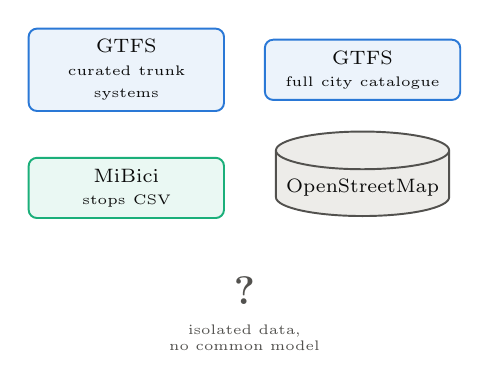
\begin{tikzpicture}[x=1cm,y=1cm]
      \node[box=cBlue, text width=2.2cm] (a) at (0,2.4) {GTFS\\ \tiny curated trunk systems};
      \node[box=cBlue, text width=2.2cm] (b) at (3.0,2.4) {GTFS\\ \tiny full city catalogue};
      \node[box=cAqua, text width=2.2cm] (c) at (0,0.9) {MiBici\\ \tiny stops CSV};
      \node[db, minimum width=2.2cm] (d) at (3.0,0.9) {OpenStreetMap};
      \node[font=\Large\bfseries, text=cInkTwo] at (1.5,-0.4) {?};
      \node[lbl, align=center] at (1.5,-1.0) {isolated data,\\no common model};
    \end{tikzpicture}
  \end{columns}
\end{frame}

% ============================================================================
\begin{frame}{What is a GTFS feed?}
  \framesubtitle{The General Transit Feed Specification: a \code{.zip} of related tables}
  \vskip0.2cm
  \centering
  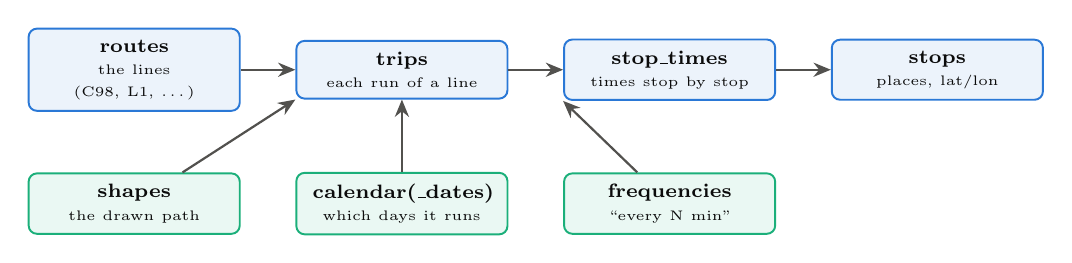
\begin{tikzpicture}[x=1cm,y=1cm]
    \node[box=cBlue, text width=2.4cm] (routes) at (0,0) {\textbf{routes}\\ \tiny the lines (C98, L1, \ldots)};
    \node[box=cBlue, text width=2.4cm] (trips) at (3.4,0) {\textbf{trips}\\ \tiny each run of a line};
    \node[box=cBlue, text width=2.4cm] (st) at (6.8,0) {\textbf{stop\_times}\\ \tiny times stop by stop};
    \node[box=cBlue, text width=2.4cm] (stops) at (10.2,0) {\textbf{stops}\\ \tiny places, lat/lon};
    \node[box=cAqua, text width=2.4cm] (cal) at (3.4,-1.7) {\textbf{calendar(\_dates)}\\ \tiny which days it runs};
    \node[box=cAqua, text width=2.4cm] (freq) at (6.8,-1.7) {\textbf{frequencies}\\ \tiny ``every N min''};
    \node[box=cAqua, text width=2.4cm] (shapes) at (0,-1.7) {\textbf{shapes}\\ \tiny the drawn path};
    \draw[arr] (routes) -- (trips); \draw[arr] (trips) -- (st); \draw[arr] (st) -- (stops);
    \draw[arr] (cal) -- (trips); \draw[arr] (freq) -- (st.south west);
    \draw[arr] (shapes) -- (trips.south west);
  \end{tikzpicture}
  \vskip0.45cm
  \small
  \renewcommand{\arraystretch}{1.25}
  \begin{tabularx}{\textwidth}{@{}l >{\raggedright\arraybackslash}X r r@{}}
    \hline
    \textbf{Source} & \textbf{What it is} & \textbf{Routes} & \textbf{Stops} \\ \hline
    \code{improved_gtfs_mimacro_mitren_sitren} & curated trunk systems, calendar 2020--2022 & 40 & 1,634 \\
    \code{mdb_2366_202502241922} & the whole city network, calendar 2024 & 276 & 12,231 \\
    \code{mibici} & bike-share docks: \code{id, name, latitude, longitude} & --- & 484 \\
    OpenStreetMap & streets and transit nodes, in PostGIS & & \\ \hline
  \end{tabularx}
\end{frame}

% ============================================================================
\begin{frame}{What the pipeline does}
  \framesubtitle{Four phases --- each command consumes what the previous one wrote}
  \vskip0.2cm
  \centering
  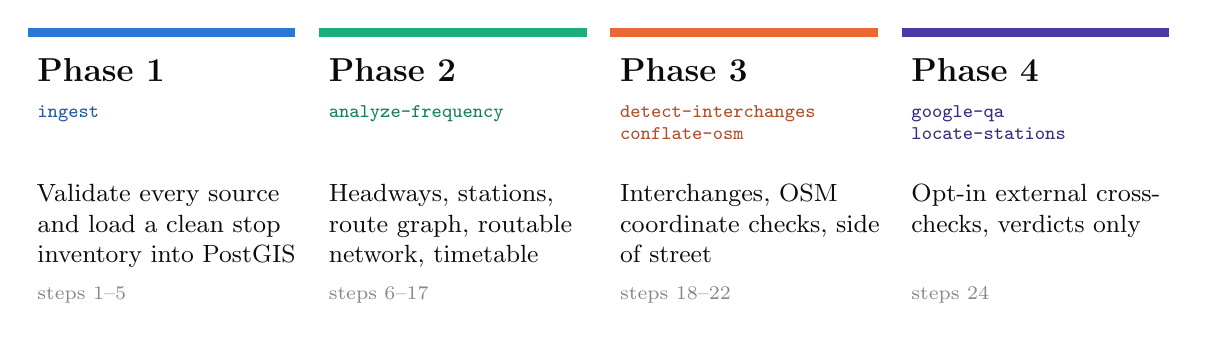
\begin{tikzpicture}[x=1cm,y=1cm]
    \foreach \i/\col/\name/\cmd/\what/\steps in {
      0/cPOne/Phase 1/ingest/Validate every source and load a clean stop inventory into PostGIS/1--5,
      1/cPTwo/Phase 2/analyze-frequency/{Headways, stations, route graph, routable network, timetable}/6--17,
      2/cPThree/Phase 3/detect-interchanges\\conflate-osm/{Interchanges, OSM coordinate checks, side of street}/18--22,
      3/cPFour/Phase 4/google-qa\\locate-stations/{Opt-in external cross-checks, verdicts only}/24}
    {
      \begin{scope}[xshift=\i*3.7cm]
        \fill[\col] (0,0) rectangle (3.4,0.12);
        \node[anchor=north west, font=\large\bfseries, text=cInk] at (0,-0.15) {\name};
        \node[anchor=north west, font=\scriptsize\ttfamily, text=\col!75!black, align=left] at (0,-0.75) {\cmd};
        \node[anchor=north west, font=\small, text=cInk, text width=3.3cm, align=left] at (0,-1.75) {\what};
        \node[anchor=north west, font=\scriptsize, text=cMuted] at (0,-3.05) {steps \steps};
      \end{scope}
    }
  \end{tikzpicture}
  \vskip0.15cm
  \begin{columns}[T]
    \column{0.24\textwidth}\centering\stat{14,349}{stop records}{cBlue}
    \column{0.24\textwidth}\centering\stat{10,203}{physical stations}{cAqua}
    \column{0.24\textwidth}\centering\stat{249}{lines in the routing network}{cOrange}
    \column{0.24\textwidth}\centering\stat{3.29\,M}{timetable connections}{cViolet}
  \end{columns}
\end{frame}

% ============================================================================
\begin{frame}{The pipeline at a glance}
  \centering
  \resizebox{\textwidth}{!}{%
  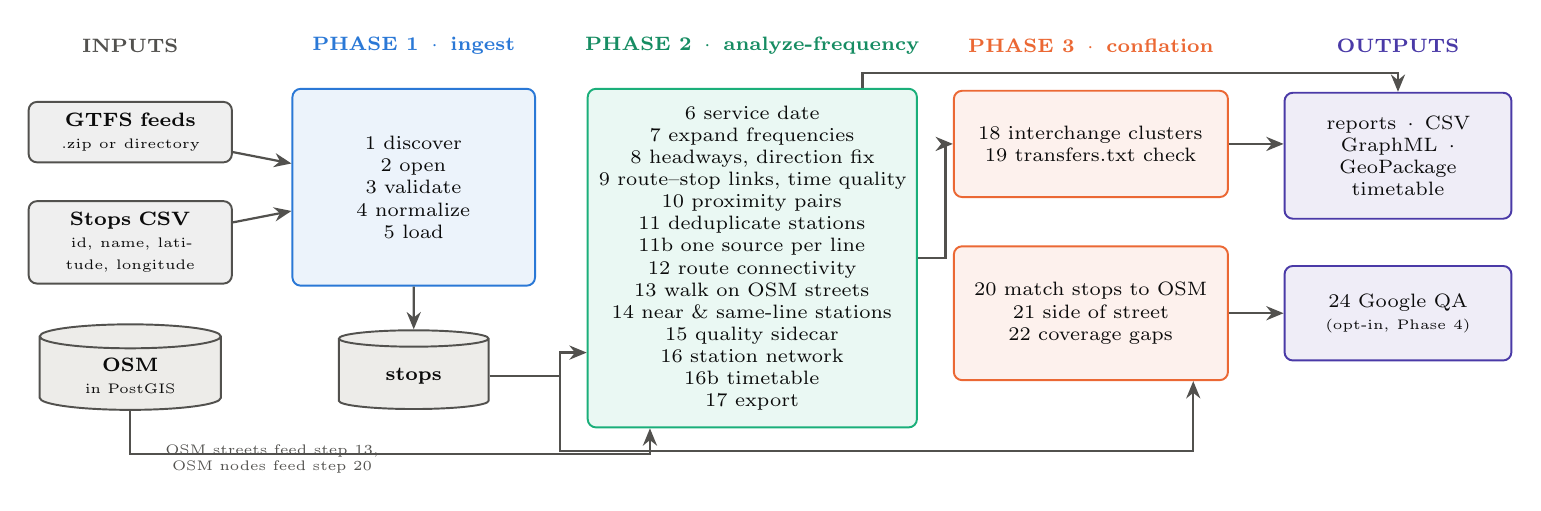
\begin{tikzpicture}[x=1cm,y=1cm]
    % inputs
    \node[lbl, font=\scriptsize\bfseries] at (0,4.3) {INPUTS};
    \node[box, text width=2.3cm] (gtfs) at (0,3.2) {\textbf{GTFS feeds}\\ \tiny .zip or directory};
    \node[box, text width=2.3cm] (csv) at (0,1.8) {\textbf{Stops CSV}\\ \tiny id, name, latitude, longitude};
    \node[db, minimum width=2.3cm] (osm) at (0,0.1) {\textbf{OSM}\\ \tiny in PostGIS};
    % phase 1
    \node[lbl, font=\scriptsize\bfseries, text=cPOne] at (3.6,4.3) {PHASE 1 \,$\cdot$\, ingest};
    \node[box=cPOne, text width=2.8cm, minimum height=2.5cm] (p1) at (3.6,2.5)
      {1 discover\\2 open\\3 validate\\4 normalize\\5 load};
    \node[db] (stops) at (3.6,0.1) {\textbf{stops}};
    % phase 2
    \node[lbl, font=\scriptsize\bfseries, text=cPTwo!80!black] at (7.9,4.3) {PHASE 2 \,$\cdot$\, analyze-frequency};
    \node[box=cPTwo, text width=3.9cm, minimum height=4.3cm] (p2) at (7.9,1.6)
      {6 service date\\7 expand frequencies\\8 headways, direction fix\\9 route--stop links, time quality
       \\10 proximity pairs\\11 deduplicate stations\\11b one source per line\\12 route connectivity
       \\13 walk on OSM streets\\14 near \& same-line stations\\15 quality sidecar\\16 station network
       \\16b timetable\\17 export};
    % phase 3
    \node[lbl, font=\scriptsize\bfseries, text=cPThree] at (12.2,4.3) {PHASE 3 \,$\cdot$\, conflation};
    \node[box=cPThree, text width=3.2cm, minimum height=1.35cm] (p3a) at (12.2,3.05)
      {18 interchange clusters\\19 transfers.txt check};
    \node[box=cPThree, text width=3.2cm, minimum height=1.7cm] (p3b) at (12.2,0.9)
      {20 match stops to OSM\\21 side of street\\22 coverage gaps};
    % outputs
    \node[lbl, font=\scriptsize\bfseries, text=cPFour] at (16.1,4.3) {OUTPUTS};
    \node[box=cPFour, text width=2.6cm, minimum height=1.6cm] (files) at (16.1,2.9)
      {reports \,$\cdot$\, CSV\\GraphML \,$\cdot$\, GeoPackage\\timetable};
    \node[box=cPFour, text width=2.6cm, minimum height=1.2cm] (neo) at (16.1,0.9)
      {24 Google QA\\ \tiny(opt-in, Phase 4)};
    % flow
    \draw[arr] (gtfs) -- (p1);
    \draw[arr] (csv) -- (p1);
    \draw[arr] (p1) -- (stops);
    \draw[arr] (stops.east) -- ++(0.9,0) |- ([yshift=-1.2cm]p2.west);
    \draw[arr] (osm.south) -- ++(0,-0.55) -| ([xshift=-1.3cm]p2.south);
    \draw[arr] (stops.east) -- ++(0.9,0) -- ++(0,-0.95) -| ([xshift=1.3cm]p3b.south) ;
    \draw[arr] (p2.east) -- ++(0.35,0) |- (p3a.west);
    \draw[arr] ([xshift=1.4cm]p2.north) |- (16.1,3.95) -- (files.north);
    \draw[arr] (p3a.east) -- (files.west |- p3a.east);
    \draw[arr] (p3b.east) -- (neo.west |- p3b.east);
    \node[lbl, align=center] at (1.8,-0.95) {OSM streets feed step 13,\\OSM nodes feed step 20};
  \end{tikzpicture}}
\end{frame}

% ============================================================================
\begin{frame}[fragile]{Run order and data lineage}
  \framesubtitle{Why \code{analyze-frequency} runs twice}
  \begin{columns}[T]
    \column{0.52\textwidth}
    \centering
    \resizebox{!}{0.74\textheight}{%
    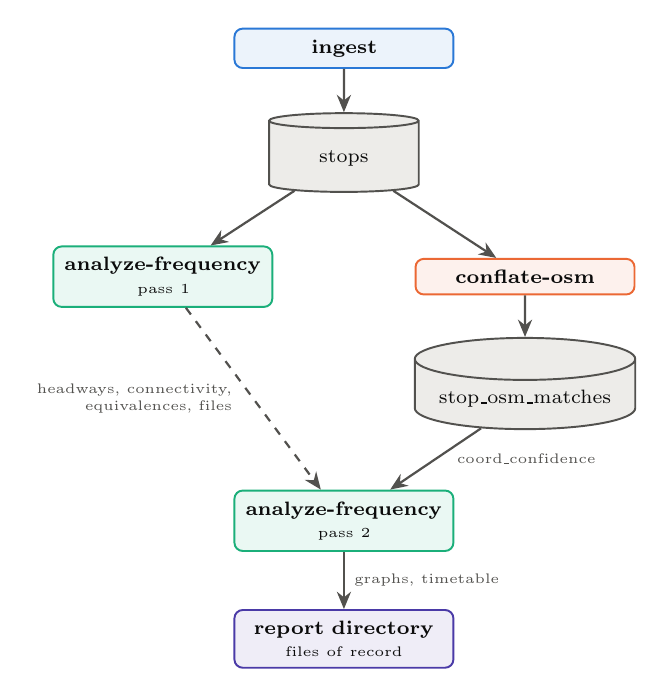
\begin{tikzpicture}[x=1cm,y=1cm]
      \node[box=cPOne, text width=2.5cm] (ing) at (0,6) {\textbf{ingest}};
      \node[db] (t1) at (0,4.6) {stops};
      \node[box=cPTwo, text width=2.5cm] (a1) at (-2.3,3.1) {\textbf{analyze-frequency}\\ \tiny pass 1};
      \node[box=cPThree, text width=2.5cm] (co) at (2.3,3.1) {\textbf{conflate-osm}};
      \node[db, minimum width=2.8cm] (t4) at (2.3,1.55) {stop\_osm\_matches};
      \node[box=cPTwo, text width=2.5cm] (a2) at (0,0) {\textbf{analyze-frequency}\\ \tiny pass 2};
      \node[box=cPFour, text width=2.5cm] (neo) at (0,-1.5) {\textbf{report directory}\\ \tiny files of record};
      \draw[arr] (ing) -- (t1);
      \draw[arr] (t1) -- (a1);
      \draw[arr] (t1) -- (co);
      \draw[arr] (co) -- (t4);
      \draw[arr] (t4) -- node[lbl, right, xshift=4pt] {coord\_confidence} (a2);
      \draw[darr] (a1) -- node[lbl, left, align=right, xshift=-4pt] {headways, connectivity,\\equivalences, files} (a2);
      \draw[arr] (a2) -- node[lbl, right] {graphs, timetable} (neo);
    \end{tikzpicture}}
    \column{0.46\textwidth}
    \small
    \begin{itemize}
      \item Each command reads what an earlier one wrote.
      \item The quality sidecar needs OSM verdicts that only \code{conflate-osm} writes
            $\Rightarrow$ a second, cached \code{analyze-frequency} pass folds them in.
      \item \code{detect-interchanges} is independent and can run anywhere after ingest.
    \end{itemize}
\begin{lstlisting}[style=algo]
ingest              --feeds $FEEDS
analyze-frequency   --feeds $FEEDS \
    --network-walk --proximity-m 300
detect-interchanges --feeds $FEEDS
conflate-osm
analyze-frequency   ...   # pass 2
\end{lstlisting}
  \end{columns}
\end{frame}

% ============================================================================
\section{Concepts}
\divider{Concepts}{cInkTwo}{Rules every step follows}{%
  Identity and provenance \,$\cdot$\, coordinate systems \,$\cdot$\, failure isolation
  \\[4pt] idempotent re-runs \,$\cdot$\, records versus stations}

% ============================================================================
\begin{frame}{Identity and provenance}
  \framesubtitle{Every identifier is qualified by the source it came from}
  \centering
  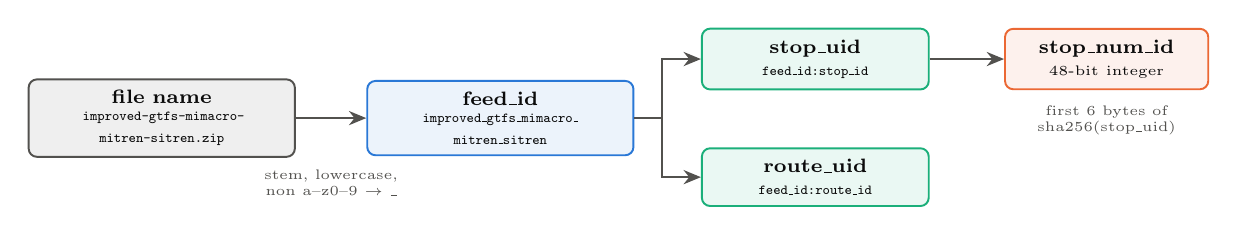
\begin{tikzpicture}[x=1cm,y=1cm]
    \node[box, text width=3.1cm] (f) at (0,0) {\textbf{file name}\\ \tiny\ttfamily improved-gtfs-mimacro-\\mitren-sitren.zip};
    \node[box=cBlue, text width=3.1cm] (id) at (4.3,0) {\textbf{feed\_id}\\ \tiny\ttfamily improved\_gtfs\_mimacro\_\\mitren\_sitren};
    \node[box=cAqua, text width=2.6cm] (su) at (8.3,0.75) {\textbf{stop\_uid}\\ \tiny\ttfamily feed\_id:stop\_id};
    \node[box=cAqua, text width=2.6cm] (ru) at (8.3,-0.75) {\textbf{route\_uid}\\ \tiny\ttfamily feed\_id:route\_id};
    \node[box=cOrange, text width=2.3cm] (num) at (12.0,0.75) {\textbf{stop\_num\_id}\\ \tiny 48-bit integer};
    \draw[arr] (f) -- (id);
    \node[lbl, align=center, below=1pt of $(f.south)!0.5!(id.south)$] {stem, lowercase,\\non a--z0--9 $\rightarrow$ \_};
    \draw[arr] (id.east) -- ++(0.35,0) |- (su);
    \draw[arr] (id.east) -- ++(0.35,0) |- (ru);
    \draw[arr] (su) -- (num);
    \node[lbl, align=center, below=2pt of num] {first 6 bytes of\\sha256(stop\_uid)};
  \end{tikzpicture}
  \vskip0.3cm
  \begin{columns}[T]
    \column{0.48\textwidth}
    \begin{block}{Guarantees}
      \small
      \begin{itemize}
        \item \code{feed_id} never contains \code{:}, so \code{stop_uid} splits back cleanly
        \item A CSV \code{S1} and a GTFS \code{S1} coexist --- different \code{stop_uid}
        \item Same path $\Rightarrow$ same id, run after run
      \end{itemize}
    \end{block}
    \column{0.48\textwidth}
    \begin{block}{Collisions}
      \small
      \begin{itemize}
        \item Two sources with the same name: add 8 hex characters of \code{sha256(path)}
        \item \code{stop_num_id} collision odds $\approx n^2/2^{49}$ --- about $10^{-4}$ at 150,000 stops;
              a unique index turns one into a load error, never silent corruption
      \end{itemize}
    \end{block}
  \end{columns}
\end{frame}

% ============================================================================
\begin{frame}{Coordinate systems and failure isolation}
  \begin{columns}[T]
    \column{0.47\textwidth}
    \textbf{Which coordinate system, where}
    \vskip0.2cm
    \small
    \renewcommand{\arraystretch}{1.35}
    \begin{tabularx}{\linewidth}{@{}>{\raggedright\arraybackslash}X >{\raggedright\arraybackslash}p{2.2cm}@{}}
      \hline
      \textbf{Use} & \textbf{CRS} \\ \hline
      Data at rest: database and files & EPSG:4326 \\
      Planar maths: DBSCAN, local proximity, walk graph, side of street & UTM, auto-detected (32613) \\
      Authoritative distances & PostGIS \code{geography} \\
      OSM layers & read from the data (3857) \\ \hline
    \end{tabularx}
    \column{0.5\textwidth}
    \textbf{A broken feed never stops a run}
    \vskip0.2cm
    \centering
    \resizebox{\linewidth}{!}{%
    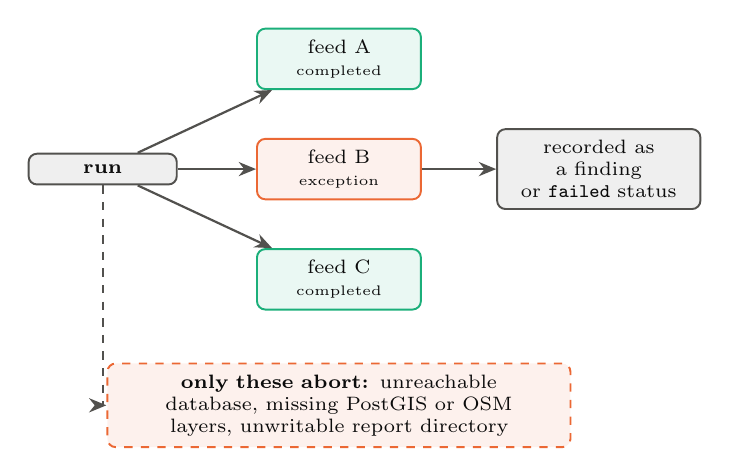
\begin{tikzpicture}[x=1cm,y=1cm]
      \node[box, text width=1.6cm] (run) at (0,0) {\textbf{run}};
      \node[box=cAqua, text width=1.8cm] (a) at (3,1.4) {feed A \\ \tiny completed};
      \node[box=cOrange, text width=1.8cm] (b) at (3,0) {feed B \\ \tiny exception};
      \node[box=cAqua, text width=1.8cm] (c) at (3,-1.4) {feed C \\ \tiny completed};
      \node[box, text width=2.3cm] (rec) at (6.3,0) {recorded as a finding\\or \code{failed} status};
      \draw[arr] (run) -- (a); \draw[arr] (run) -- (b); \draw[arr] (run) -- (c);
      \draw[arr] (b) -- (rec);
      \node[box=cOrange, text width=5.6cm, dashed] (ab) at (3,-3.0)
        {\textbf{only these abort:} unreachable database, missing PostGIS or OSM layers,
         unwritable report directory};
      \draw[darr] (run.south) |- (ab.west);
    \end{tikzpicture}}
  \end{columns}
\end{frame}

% ============================================================================
\begin{frame}{Idempotency: how a re-run replaces data}
  \framesubtitle{Re-running any command is always safe --- but the strategy depends on the table}
  \vskip0.2cm
  \centering
  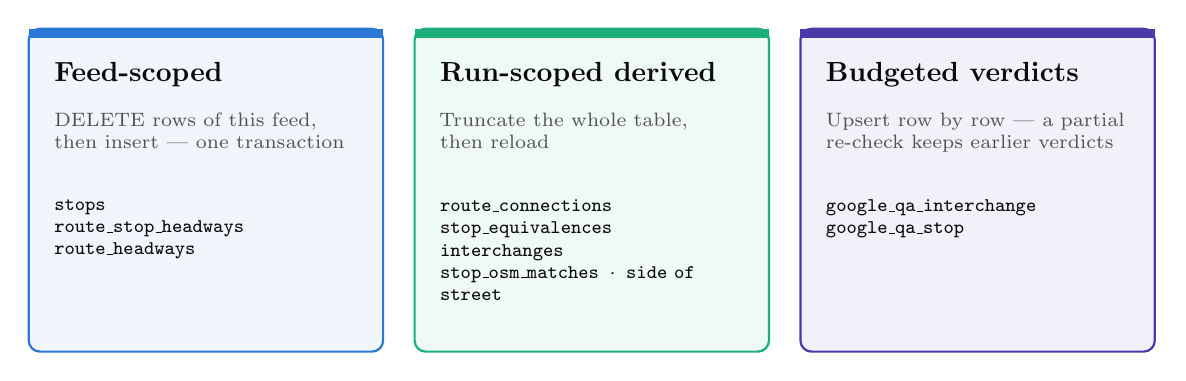
\begin{tikzpicture}[x=1cm,y=1cm]
    \foreach \x/\col/\title/\how/\tables in {
      0/cBlue/Feed-scoped/{DELETE rows of this feed,\\then insert --- one transaction}/stops\\route\_stop\_headways\\route\_headways,
      4.9/cAqua/Run-scoped derived/{Truncate the whole table,\\then reload}/route\_connections\\stop\_equivalences\\interchanges\\stop\_osm\_matches \,$\cdot$\, side of street,
      9.8/cViolet/Budgeted verdicts/Upsert row by row --- a partial\\re-check keeps earlier verdicts/google\_qa\_interchange\\google\_qa\_stop}
    {
      \node[draw=\col, fill=\col!7, line width=0.8pt, rounded corners=4pt, minimum width=4.5cm,
            minimum height=4.1cm] at (\x+2.25,-2.05) {};
      \fill[\col] (\x,0) rectangle ++(4.5,-0.12);
      \node[anchor=north west, font=\bfseries, text=cInk] at (\x+0.2,-0.3) {\title};
      \node[anchor=north west, font=\scriptsize, text=cInkTwo, align=left, text width=4.1cm] at (\x+0.2,-0.95) {\how};
      \node[anchor=north west, font=\scriptsize\ttfamily, text=cInk, align=left, text width=4.1cm] at (\x+0.2,-2.05) {\tables};
    }
  \end{tikzpicture}
  \vskip0.35cm
  \begin{alertblock}{Consequence}
    \small For run-scoped tables, pass \textbf{every} source you care about in one run: a run with two feeds
    leaves only those two feeds' connections in \code{route_connections}.
  \end{alertblock}
\end{frame}

% ============================================================================
\begin{frame}[fragile]{Records are not stations}
  \framesubtitle{Deduplication records equivalences --- it never deletes a row}
  \begin{columns}[c]
    \column{0.62\textwidth}
    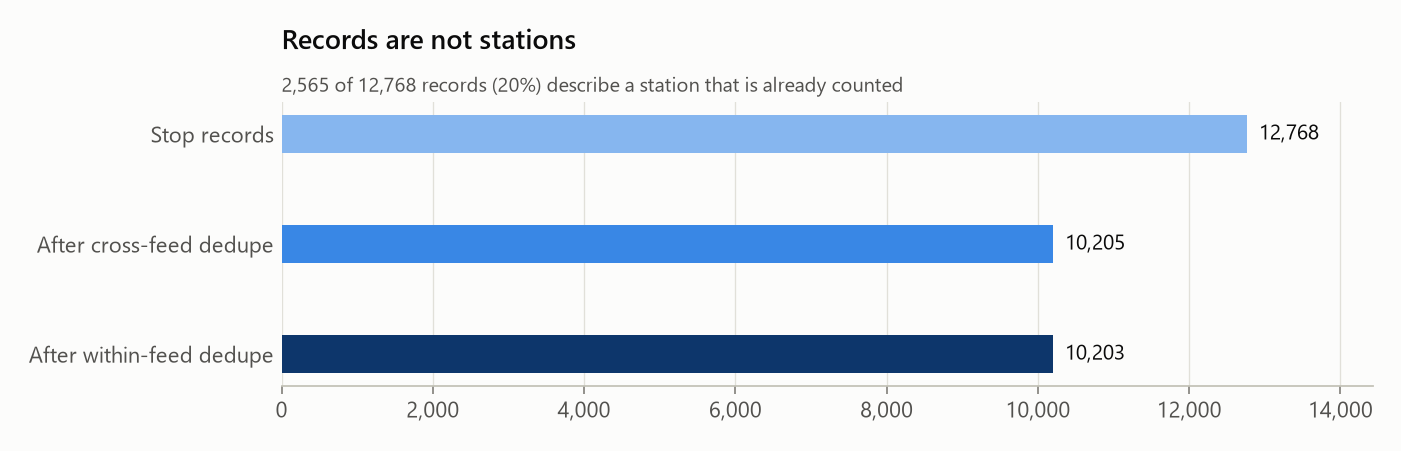
\includegraphics[width=\linewidth]{r1_records_to_stations.png}
    \column{0.36\textwidth}
    \small
    A raw \code{COUNT(*)} counts \textbf{records}. To count \textbf{physical stations}, resolve each record
    to its group with \code{station_dedup} from \code{near_stations_quality.csv}:
\begin{lstlisting}[style=sql]
COUNT(DISTINCT COALESCE(
  NULLIF(station_dedup, ''),
  stop_uid))
\end{lstlisting}
    \muted{12,768 served records are 10,203 stations: any density or coverage figure on raw records
    is inflated by $\approx$1.25$\times$.}
  \end{columns}
\end{frame}

% ============================================================================
\section{Phase 1 --- Ingest}
\divider{Phase 1 \,$\cdot$\, Ingest}{cPOne}{\code{ingest} --- a clean, validated stop inventory in PostGIS}{%
  \textbf{1} Discover sources \quad \textbf{2} Open each source \quad \textbf{3} Validate
  \quad \textbf{4} Normalize stops \quad \textbf{5} Load into PostGIS}

% ============================================================================
\begin{frame}{\step{cPOne}{1}Discover sources}
  \framesubtitle{Every path is classified once, and the kind is fixed at that moment}
  \begin{columns}[T]
    \column{0.6\textwidth}
    \centering
    \resizebox{!}{0.76\textheight}{%
    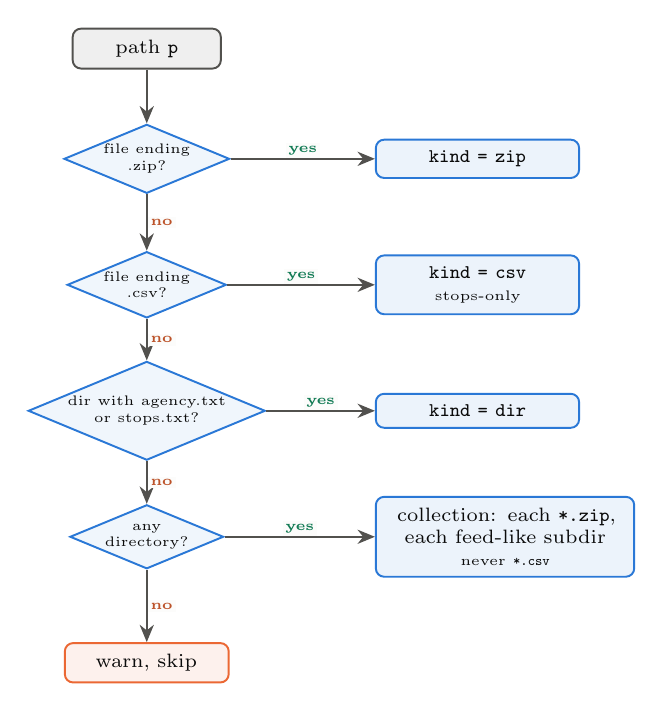
\begin{tikzpicture}[x=1cm,y=1cm]
      \node[box, text width=1.6cm] (p) at (0,0) {path \code{p}};
      \node[dec=cPOne] (z) at (0,-1.4) {file ending\\.zip?};
      \node[dec=cPOne] (c) at (0,-3.0) {file ending\\.csv?};
      \node[dec=cPOne] (d) at (0,-4.6) {dir with agency.txt\\or stops.txt?};
      \node[dec=cPOne] (e) at (0,-6.2) {any\\directory?};
      \node[box=cPOne, text width=2.3cm] (kz) at (4.2,-1.4) {\code{kind = zip}};
      \node[box=cPOne, text width=2.3cm] (kc) at (4.2,-3.0) {\code{kind = csv}\\ \tiny stops-only};
      \node[box=cPOne, text width=2.3cm] (kd) at (4.2,-4.6) {\code{kind = dir}};
      \node[box=cPOne, text width=3.0cm] (col) at (4.55,-6.2) {collection: each \code{*.zip}, each feed-like subdir\\ \tiny never \code{*.csv}};
      \node[box=cOrange, text width=1.8cm] (sk) at (0,-7.8) {warn, skip};
      \draw[arr] (p) -- (z);
      \draw[arr] (z) -- node[yes, above] {yes} (kz);
      \draw[arr] (z) -- node[no, right] {no} (c);
      \draw[arr] (c) -- node[yes, above] {yes} (kc);
      \draw[arr] (c) -- node[no, right] {no} (d);
      \draw[arr] (d) -- node[yes, above] {yes} (kd);
      \draw[arr] (d) -- node[no, right] {no} (e);
      \draw[arr] (e) -- node[yes, above] {yes} (col);
      \draw[arr] (e) -- node[no, right] {no} (sk);
    \end{tikzpicture}}
    \column{0.38\textwidth}
    \small
    \textbf{Output:} a list of \code{FeedSource(feed_id, path, kind)}, de-duplicated by resolved path.
    \vskip0.35cm
    \begin{alertblock}{Why a CSV must be named explicitly}
      \scriptsize The pipeline's own \code{near_stations.csv} has \code{ID}, \code{stop_lat} and
      \code{stop_lon} --- a \emph{valid} stops CSV. Scanning folders for CSVs would silently re-ingest a
      previous run's output as a second copy of the network.
    \end{alertblock}
    \vskip0.2cm
    \muted{\scriptsize A directory named \code{foo.zip} stays a directory: the kind comes from the layout, not the suffix.}
  \end{columns}
\end{frame}

% ============================================================================
\begin{frame}{\step{cPOne}{2}Open each source}
  \framesubtitle{Two ways in, one object out --- every later step reads both the same way}
  \centering
  \resizebox{\textwidth}{!}{%
  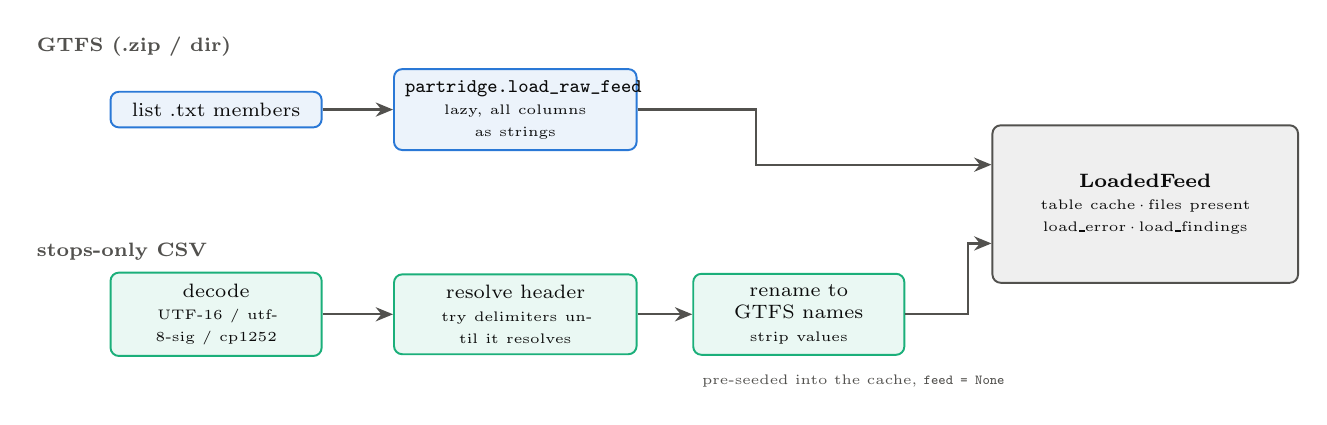
\begin{tikzpicture}[x=1cm,y=1cm]
    \node[lbl, font=\scriptsize\bfseries, anchor=west] at (-1.2,2.0) {GTFS (.zip / dir)};
    \node[box=cPOne, text width=2.4cm] (g1) at (1.2,1.2) {list .txt members};
    \node[box=cPOne, text width=2.8cm] (g2) at (5.0,1.2) {\code{partridge.load_raw_feed}\\ \tiny lazy, all columns as strings};
    \node[lbl, font=\scriptsize\bfseries, anchor=west] at (-1.2,-0.6) {stops-only CSV};
    \node[box=cAqua, text width=2.4cm] (c1) at (1.2,-1.4) {decode\\ \tiny UTF-16 / utf-8-sig / cp1252};
    \node[box=cAqua, text width=2.8cm] (c2) at (5.0,-1.4) {resolve header\\ \tiny try delimiters until it resolves};
    \node[box=cAqua, text width=2.4cm] (c3) at (8.6,-1.4) {rename to GTFS names\\ \tiny strip values};
    \node[box, text width=3.6cm, minimum height=2.0cm] (lf) at (13.0,0) {\textbf{LoadedFeed}\\[2pt] \tiny table cache\,$\cdot$\,files present\\ \tiny load\_error\,$\cdot$\,load\_findings};
    \draw[arr] (g1) -- (g2);
    \draw[arr] (g2.east) -- ++(1.5,0) |- ([yshift=0.5cm]lf.west);
    \draw[arr] (c1) -- (c2);
    \draw[arr] (c2) -- (c3);
    \draw[arr] (c3.east) -- ++(0.8,0) |- ([yshift=-0.5cm]lf.west);
    \node[lbl, anchor=north west] at ([yshift=-0.12cm]c3.south west) {pre-seeded into the cache, \code{feed = None}};
  \end{tikzpicture}}
  \vskip0.25cm
  \begin{columns}[T]
    \column{0.48\textwidth}
    \begin{block}{Why read raw strings?}
      \small Validation must see the file \emph{exactly as published}. Typing happens later, explicitly,
      in normalization.
    \end{block}
    \column{0.48\textwidth}
    \begin{exampleblock}{Why pre-seed the CSV?}
      \small Table access consults the cache before the partridge object, so validators, the normalizer
      and Phase 2 read a CSV source with \textbf{no special cases}.
    \end{exampleblock}
  \end{columns}
\end{frame}

% ============================================================================
\begin{frame}[fragile]{\step{cPOne}{2}The stops-CSV reader: forgiving, never guessing}
  \begin{columns}[T]
    \column{0.47\textwidth}
    \textbf{Header resolution}
\begin{lstlisting}[style=algo]
normalize(cell) =
    strip BOM and quotes
    -> NFKD, drop accents -> casefold
    -> non-alphanumeric runs -> "_"

for each delimiter candidate:
    parse (all values as strings)
    map normalize(cell) -> canonical
    if stop_id, stop_lat, stop_lon found:
        accept          # first match wins
# none resolved -> ERROR unresolved_csv_header
\end{lstlisting}
    \vskip0.1cm
    \scriptsize
    \textbf{Examples:} \code{Latitud}, \code{LATITUDE}, \code{lat} $\rightarrow$ \code{stop_lat}
    \quad \texttt{ESTACI\'ON} $\rightarrow$ \code{stop_name}
    \column{0.5\textwidth}
    \small
    \renewcommand{\arraystretch}{1.3}
    \begin{tabularx}{\linewidth}{@{}l>{\raggedright\arraybackslash}X@{}}
      \hline
      \textbf{Canonical} & \textbf{Accepted spellings} \\ \hline
      \code{stop_id}   & id, stop\_id, stopid, codigo, clave \\
      \code{stop_name} & name, stop\_name, stopname, nombre, estacion \\
      \code{stop_lat}  & latitude, lat, stop\_lat, latitud \\
      \code{stop_lon}  & longitude, lon, lng, long, stop\_lon, longitud \\ \hline
    \end{tabularx}
    \vskip0.3cm
    \begin{itemize}\scriptsize
      \item \textbf{utf-8-sig first:} Spanish-locale Excel writes \code{;}-separated UTF-8 with a BOM
      \item \textbf{Decimal commas} (\code{20,6736}) are flagged, never rewritten
      \item Unknown columns such as MiBici's \code{dpcapacity} are ignored
      \item The error names what was found, what is missing, and the spellings that would work
    \end{itemize}
  \end{columns}
\end{frame}

% ============================================================================
\begin{frame}{\step{cPOne}{3}Validate}
  \framesubtitle{Every check runs --- a crashing check becomes a finding, not a stopped run}
  \begin{columns}[T]
    \column{0.64\textwidth}
    \scriptsize
    \renewcommand{\arraystretch}{1.22}
    \begin{tabularx}{\linewidth}{@{}c>{\raggedright\arraybackslash}X l@{}}
      \hline
      & \textbf{Check} & \textbf{Finding} \\ \hline
      \sevE & agency, stops, routes, trips, stop\_times present & \code{missing_required_file} \\
      \sevE & calendar.txt or calendar\_dates.txt present & \code{missing_calendar} \\
      \sevE & present files parse; required files non-empty & \code{unreadable_file} \\
      \sevE & required columns per file & \code{missing_required_columns} \\
      \sevE & stops: non-null, unique \code{stop_id} & \code{duplicate_stop_ids} \\
      \sevE & stops: coordinates in WGS84 range & \code{invalid_coordinates} \\
      \sevW & \code{parent_station} references a known stop & \code{dangling_parent_station} \\
      \sevE & trips$\rightarrow$routes, stop\_times$\rightarrow$trips, stop\_times$\rightarrow$stops & \code{dangling_reference} \\
      \sevW & declared service ended before the analysis date & \code{feed_expired} \\
      \sevI  & optional-file inventory & \code{optional_files} \\ \hline
    \end{tabularx}
    \column{0.33\textwidth}
    \begin{block}{Severity policy}
      \scriptsize
      \textbf{ERROR} spec violation or data loss\\
      \textbf{WARNING} recoverable\\
      \textbf{INFO} inventory\\[3pt]
      \code{--fail-on-error} exits 2 on any ERROR.
    \end{block}
    \vskip0.2cm
    \begin{exampleblock}{Stops-only sources}
      \scriptsize The required-files check becomes one INFO \code{stops_only_source}. Every other check still
      runs --- a bad coordinate in a CSV raises the same finding as in a GTFS feed.
    \end{exampleblock}
  \end{columns}
\end{frame}

% ============================================================================
\begin{frame}{\step{cPOne}{4}Normalize stops}
  \framesubtitle{Repair by exclusion only --- a value is never guessed}
  \centering
  \resizebox{\textwidth}{!}{%
  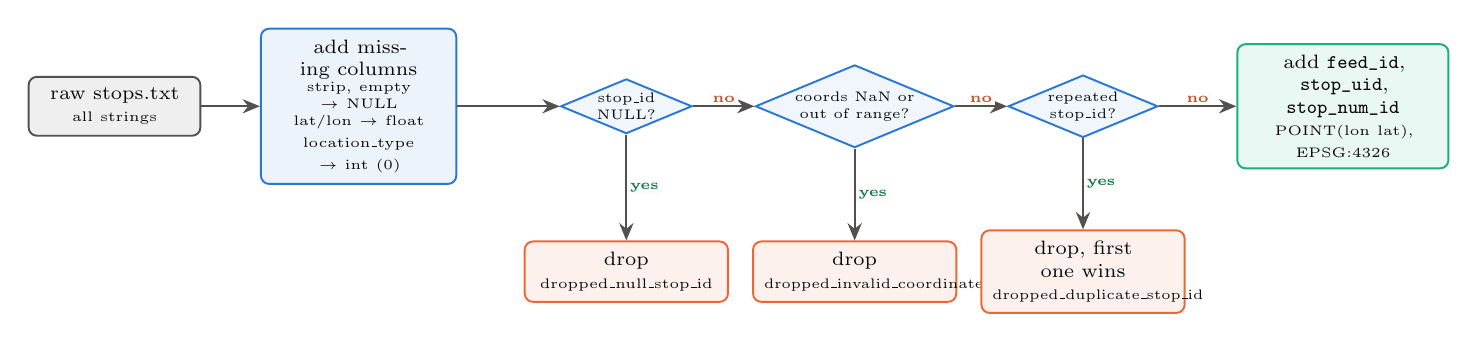
\begin{tikzpicture}[x=1cm,y=1cm]
    \node[box, text width=1.9cm] (raw) at (0,0) {raw stops.txt\\ \tiny all strings};
    \node[box=cPOne, text width=2.2cm] (t) at (3.1,0) {add missing columns\\ \tiny strip, empty $\rightarrow$ NULL\\ \tiny lat/lon $\rightarrow$ float\\ \tiny location\_type $\rightarrow$ int (0)};
    \node[dec=cPOne] (d1) at (6.5,0) {stop\_id\\NULL?};
    \node[dec=cPOne] (d2) at (9.4,0) {coords NaN or\\out of range?};
    \node[dec=cPOne] (d3) at (12.3,0) {repeated\\stop\_id?};
    \node[box=cAqua, text width=2.4cm] (id) at (15.6,0) {add \code{feed_id}, \code{stop_uid}, \code{stop_num_id}\\ \tiny POINT(lon lat), EPSG:4326};
    \node[box=cOrange, text width=2.3cm] (x1) at (6.5,-2.1) {drop\\ \tiny dropped\_null\_stop\_id};
    \node[box=cOrange, text width=2.3cm] (x2) at (9.4,-2.1) {drop\\ \tiny dropped\_invalid\_coordinates};
    \node[box=cOrange, text width=2.3cm] (x3) at (12.3,-2.1) {drop, first one wins\\ \tiny dropped\_duplicate\_stop\_id};
    \draw[arr] (raw) -- (t); \draw[arr] (t) -- (d1);
    \draw[arr] (d1) -- node[no, above] {no} (d2);
    \draw[arr] (d2) -- node[no, above] {no} (d3);
    \draw[arr] (d3) -- node[no, above] {no} (id);
    \draw[arr] (d1) -- node[yes, right] {yes} (x1);
    \draw[arr] (d2) -- node[yes, right] {yes} (x2);
    \draw[arr] (d3) -- node[yes, right] {yes} (x3);
  \end{tikzpicture}}
  \vskip0.5cm
  \begin{columns}[T]
    \column{0.5\textwidth}
    \textbf{Output columns}\\[2pt]
    \scriptsize\ttfamily stop\_uid, stop\_num\_id, feed\_id, stop\_id, stop\_name, stop\_lat, stop\_lon,
    location\_type, parent\_station, geometry
    \column{0.46\textwidth}
    \small Drop counts mirror the validator codes, so\\[2pt]
    \centering\code{source rows - dropped = normalized rows}\\[2pt]
    \raggedright is always reconstructible from the report.
  \end{columns}
\end{frame}

% ============================================================================
\begin{frame}[fragile]{\step{cPOne}{5}Load stops into PostGIS}
  \framesubtitle{Per-feed replace, bulk-copied, all inside one transaction}
  \begin{columns}[T]
    \column{0.5\textwidth}
\begin{lstlisting}[style=sql]
BEGIN;
DELETE FROM stops WHERE feed_id = :feed_id;
CREATE TEMP TABLE tmp_stops (...)
    ON COMMIT DROP;
COPY tmp_stops FROM STDIN;          -- bulk
INSERT INTO stops (..., geom)
SELECT ..., ST_SetSRID(
         ST_MakePoint(stop_lon, stop_lat), 4326)
FROM tmp_stops;
COMMIT;
\end{lstlisting}
    \column{0.47\textwidth}
    \centering
    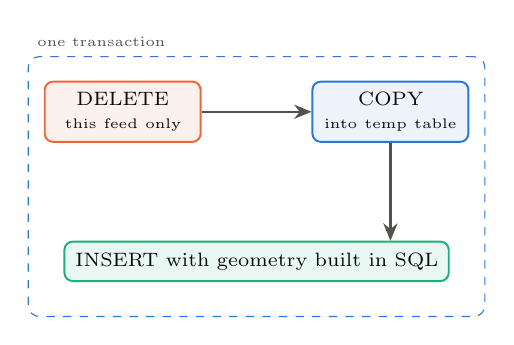
\begin{tikzpicture}[x=1cm,y=1cm]
      \node[draw=cPOne, dashed, rounded corners=4pt, minimum width=5.8cm, minimum height=3.3cm,
            label={[lbl, anchor=south west]north west:one transaction}] at (2.8,-1.35) {};
      \node[box=cOrange, text width=1.7cm] (del) at (1.1,-0.4) {DELETE\\ \tiny this feed only};
      \node[box=cPOne, text width=1.7cm] (cp) at (4.5,-0.4) {COPY\\ \tiny into temp table};
      \node[box=cAqua, text width=4.6cm] (ins) at (2.8,-2.3) {INSERT with geometry built in SQL};
      \draw[arr] (del) -- (cp); \draw[arr] (cp.south) -- (cp.south |- ins.north);
    \end{tikzpicture}
    \vskip0.2cm
    \scriptsize
    \begin{itemize}
      \item \code{COPY} fails? The same rows go through chunked \code{executemany} (1,000 per chunk) ---
            same transaction
      \item Indexes: GiST on \code{geom}, \code{feed_id}, unique \code{stop_num_id}
      \item Other feeds are never touched
    \end{itemize}
  \end{columns}
\end{frame}

% ============================================================================
\section{Phase 2 --- Service analysis}
\divider{Phase 2 \,$\cdot$\, Service analysis}{cPTwo}{\code{analyze-frequency} --- per feed, then across all feeds}{%
  \textbf{Per feed:} 6 service date \quad 7 expand frequencies \quad 8 headways \quad 9 route--stop links \& geometry\\[5pt]
  \textbf{Across feeds:} 10 proximity \quad 11 dedupe \quad 11b one source per line \quad 12 connectivity
  \quad 13 OSM walk\\[3pt] 14 near stations \quad 15 quality \quad 16 station network \quad 16b timetable \quad 17 export}

% ============================================================================
\begin{frame}{The life of one feed in Phase 2}
  \framesubtitle{Each feed runs inside its own failure boundary}
  \begin{columns}[c]
    \column{0.62\textwidth}
    \centering
    \resizebox{\linewidth}{!}{%
    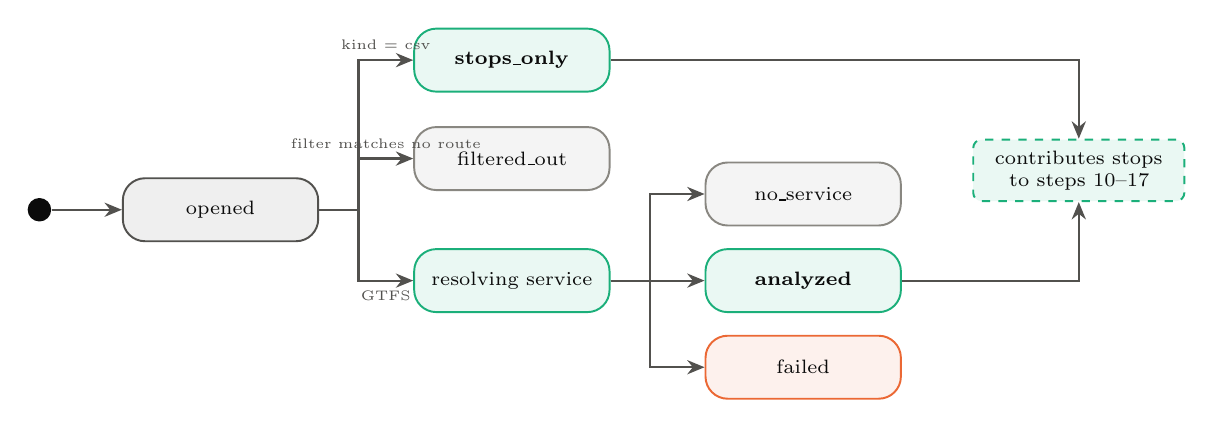
\begin{tikzpicture}[x=1cm,y=1cm, font=\small]
      \node[circle, fill=cInk, inner sep=3pt] (s) at (0,0) {};
      \node[st=cInkTwo] (op) at (2.3,0) {opened};
      \node[st=cAqua] (so) at (6.0,1.9) {\textbf{stops\_only}};
      \node[st=cMuted] (fo) at (6.0,0.65) {filtered\_out};
      \node[st=cPTwo] (rs) at (6.0,-0.9) {resolving service};
      \node[st=cMuted] (ns) at (9.7,0.2) {no\_service};
      \node[st=cAqua] (an) at (9.7,-0.9) {\textbf{analyzed}};
      \node[st=cOrange] (fa) at (9.7,-2.0) {failed};
      \node[box=cAqua, text width=2.4cm, dashed] (cs) at (13.2,0.5) {contributes stops to steps 10--17};
      \draw[arr] (s) -- (op);
      \draw[arr] (op.east) -- ++(0.5,0) |- node[lbl, pos=0.75, above] {kind = csv} (so);
      \draw[arr] (op.east) -- ++(0.5,0) |- node[lbl, pos=0.75, above] {filter matches no route} (fo);
      \draw[arr] (op.east) -- ++(0.5,0) |- node[lbl, pos=0.75, below] {GTFS} (rs);
      \draw[arr] (rs.east) -- ++(0.5,0) |- (ns);
      \draw[arr] (rs) -- (an);
      \draw[arr] (rs.east) -- ++(0.5,0) |- (fa);
      \draw[arr] (so.east) -| (cs.north);
      \draw[arr] (an.east) -| (cs.south);
    \end{tikzpicture}}
    \column{0.36\textwidth}
    \small
    \begin{exampleblock}{Stops-only sources branch out first}
      \scriptsize No calendar and no trips, so every service-date path would fail. Instead they are normalized,
      loaded and marked \code{stops_only} with no service date --- and still take part in steps 10--17.
    \end{exampleblock}
    \vskip0.2cm
    \begin{itemize}\scriptsize
      \item Exempt from \code{--transport-mode} / \code{--route}: nothing to match
      \item Excluded from \code{--common-date}: no calendar to share
      \item No service date, so they never make the run look incoherent
    \end{itemize}
  \end{columns}
\end{frame}

% ============================================================================
\begin{frame}{\step{cPTwo}{6}Resolve the service date}
  \framesubtitle{Headways depend on which trips actually run that day}
  \vskip0.1cm
  \begin{block}{Active services on a date}
    \centering\small
    $\mathit{active}(d) \;=\; \{\,s : \text{weekday flag set},\ \mathit{start} \le d \le \mathit{end}\,\}
      \;\cup\; \{\,s : \text{added on } d\,\} \;\setminus\; \{\,s : \text{removed on } d\,\}$
  \end{block}
  \vskip0.2cm
  \begin{columns}[T]
    \column{0.64\textwidth}
    \scriptsize
    \renewcommand{\arraystretch}{1.25}
    \begin{tabularx}{\linewidth}{@{}>{\raggedright\arraybackslash}p{3.3cm}>{\raggedright\arraybackslash}X@{}}
      \hline
      \textbf{Mode} & \textbf{Date chosen} \\ \hline
      \code{--service-date D} & exactly D \\
      \textbf{default}: \code{--date-rule}\newline\code{typical-weekday} & per feed: most common Mon--Fri service on days
        \code{calendar_dates} doesn't touch; middle Tue--Thu date \\
      \code{--date-rule busiest} & the date with the most trips --- a \textbf{holiday} here \\
      \code{--feed-service-date F=D} & pin one feed \\
      \code{--common-date} & $\max\bigl(\bigcap_{\text{feeds}}\{\text{served dates}\}\bigr)$; exit 1 if empty \\
      \code{--service-date-range} & every served date in the window, $\le$ 31 days \\ \hline
    \end{tabularx}
    \column{0.34\textwidth}
    \centering
    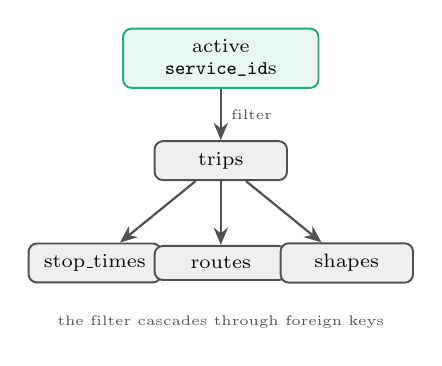
\begin{tikzpicture}[x=1cm,y=1cm]
      \node[box=cPTwo, text width=2.2cm] (v) at (0,0) {active \code{service_id}s};
      \node[box, text width=1.4cm] (t) at (0,-1.3) {trips};
      \node[box, text width=1.4cm] (st) at (-1.6,-2.6) {stop\_times};
      \node[box, text width=1.4cm] (r) at (0,-2.6) {routes};
      \node[box, text width=1.4cm] (sh) at (1.6,-2.6) {shapes};
      \draw[arr] (v) -- node[lbl, right] {filter} (t);
      \draw[arr] (t) -- (st); \draw[arr] (t) -- (r); \draw[arr] (t) -- (sh);
      \node[lbl] at (0,-3.35) {the filter cascades through foreign keys};
    \end{tikzpicture}
  \end{columns}
  \vskip0.1cm
  \muted{\scriptsize ``Busiest'' picked the holidays 2020-01-01 and 2024-01-01 (Sunday service on top of
  weekday service). Typical weekday: \textbf{2021-05-04} (improved), \textbf{2024-06-27} (mdb); the calendars
  never overlap, which \code{service_dates_note} explains.}
\end{frame}

% ============================================================================
\begin{frame}[fragile]{\step{cPTwo}{7}Expand frequencies.txt}
  \framesubtitle{A frequency-defined trip is a pattern, not a departure}
  \centering
  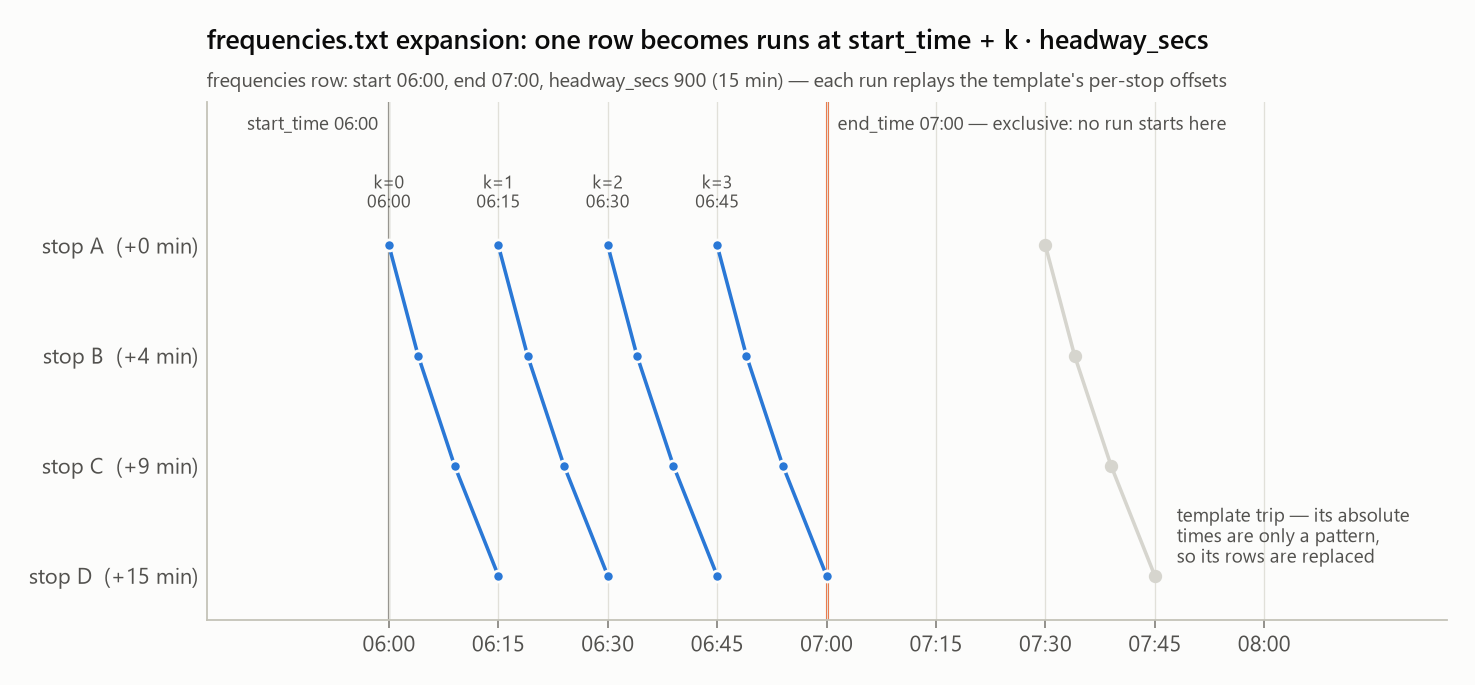
\includegraphics[width=0.68\textwidth]{e2_frequency_expansion.png}
  \vskip-0.05cm
  \begin{columns}[T]
    \column{0.57\textwidth}
\begin{lstlisting}[style=algo]
n_runs  = min(ceil((end - start) / headway), 1000)
offsets = departure(stop) - first departure
for k in 0 .. n_runs-1:
    emit (trip, stop, start + k*headway + offset)
drop duplicate rows; replace the template rows
\end{lstlisting}
    \column{0.4\textwidth}
    \scriptsize
    \begin{itemize}
      \item \code{end_time} is exclusive; invalid rows skipped with a warning
      \item Duplicates dropped: overlapping ranges would create 0-second gaps
      \item On the analysed day, \textbf{82 of 84} (improved) and \textbf{500 of 511} (mdb) trips are
            frequency templates
    \end{itemize}
  \end{columns}
\end{frame}

% ============================================================================
\begin{frame}{\step{cPTwo}{8}Compute headways}
  \framesubtitle{The gap between consecutive departures, per stop, route, direction and window}
  \centering
  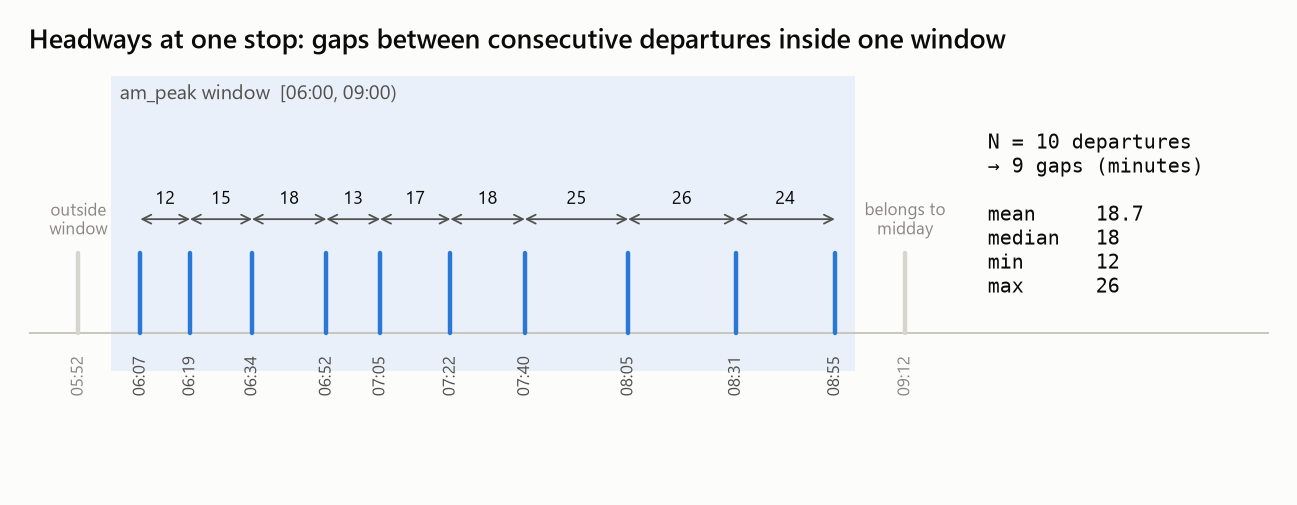
\includegraphics[width=0.74\textwidth]{e1_headway_timeline.png}
  \vskip0.05cm
  \begin{columns}[T]
    \column{0.48\textwidth}
    \begin{block}{Definition}
      \scriptsize Window $w = [\mathit{start}, \mathit{end})$ \,$\cdot$\, $N$ departures $\Rightarrow N-1$ gaps\\
      \code{mean, median, min, max} of the gaps, in seconds\\
      $N = 1$: headway undefined, statistics NULL
    \end{block}
    \column{0.48\textwidth}
    \begin{block}{Details}
      \scriptsize Default windows: am\_peak 06--09, midday 09--15, pm\_peak 15--19, evening 19--23\\
      Blank \code{direction_id} $\rightarrow -1$; directions never merged\\
      Mixed-sense routes relabelled first (next slide)
    \end{block}
  \end{columns}
\end{frame}

% ============================================================================
\begin{frame}{\step{cPTwo}{8}Route rollup --- and what the data shows}
  \begin{columns}[c]
    \column{0.36\textwidth}
    \textbf{Per route, direction and window}
    \vskip0.2cm
    \scriptsize
    \renewcommand{\arraystretch}{1.3}
    \begin{tabularx}{\linewidth}{@{}l>{\raggedright\arraybackslash}X@{}}
      \hline
      \code{mean_headway_s} & mean of stop-level means \\
      \code{stop_count} & stops with a departure \\
      \code{stops_with_headway} & stops with $\ge 2$ departures \\
      \code{trip_count} & max stop-level count \\ \hline
    \end{tabularx}
    \vskip0.25cm
    \muted{Unweighted: every stop counts equally.}
    \vskip0.35cm
    \begin{alertblock}{Read this carefully}
      \scriptsize The median is 8.0\,min in every window. The feeds define uniform frequencies all day ---
      a property of the source data, \textbf{not} a finding about the city.
    \end{alertblock}
    \column{0.62\textwidth}
    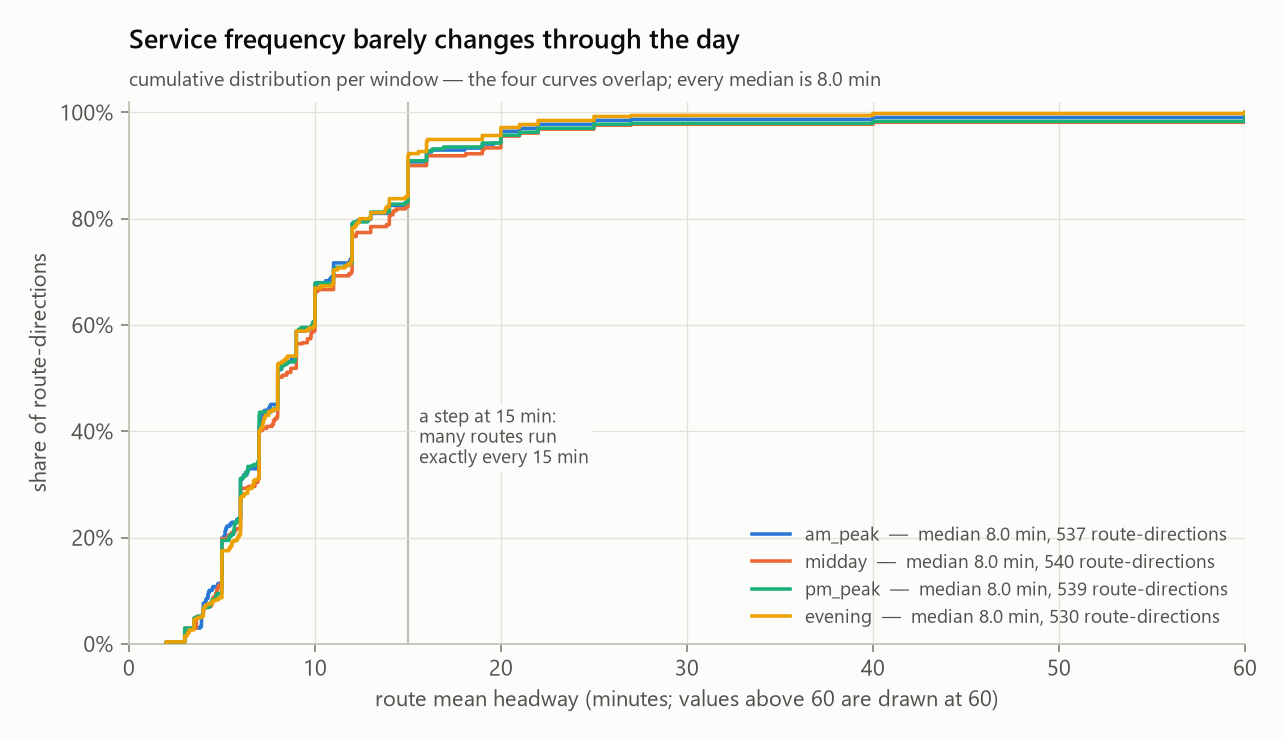
\includegraphics[width=\linewidth]{r8_headways_by_window.png}
  \end{columns}
\end{frame}

% ============================================================================
\begin{frame}{\step{cPTwo}{8}Mixed directions: relabel from stop order}
  \framesubtitle{Some routes put both senses under one \code{direction_id} --- headways then count both ways}
  \begin{columns}[c]
    \column{0.6\textwidth}
    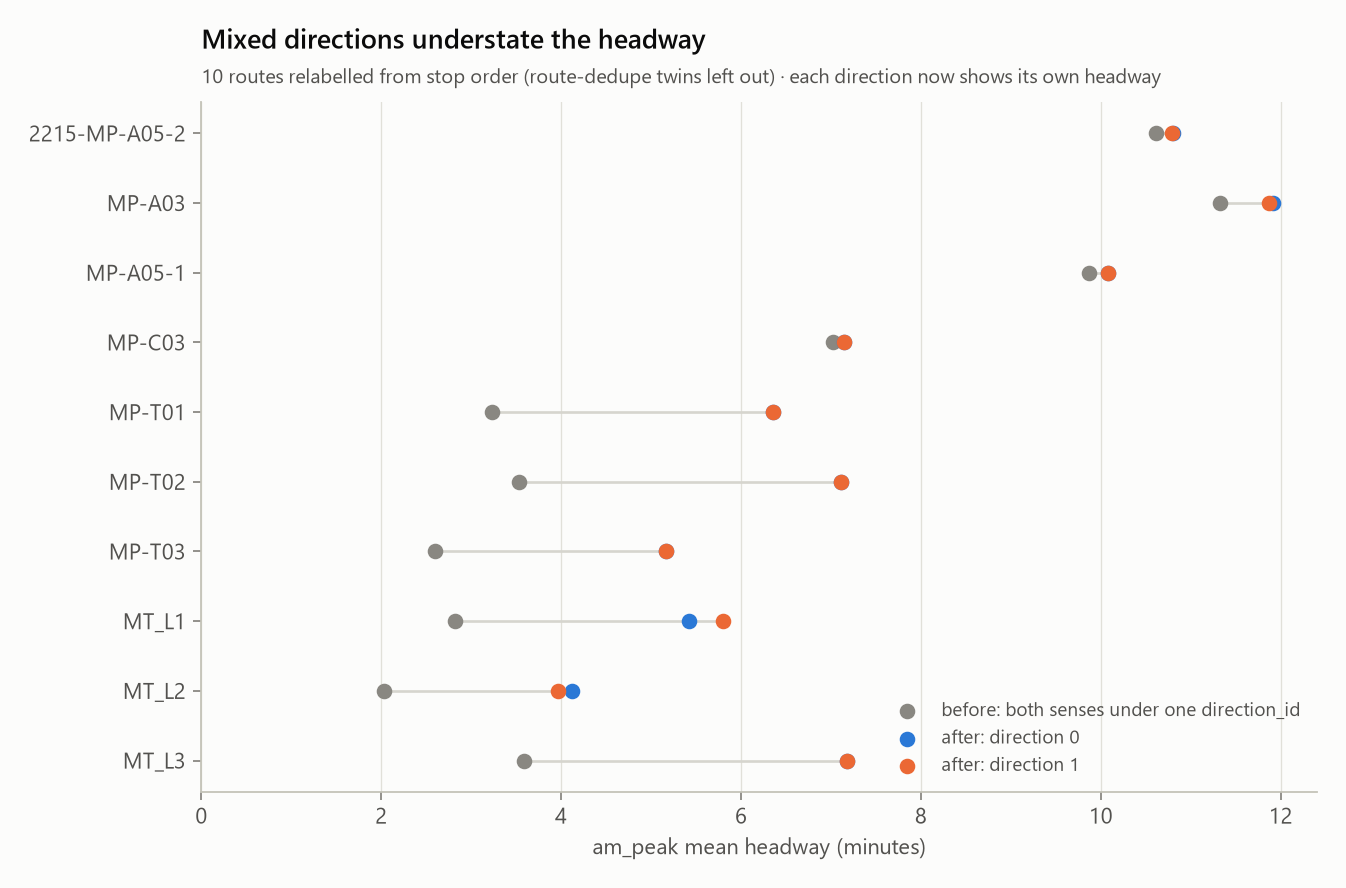
\includegraphics[width=\linewidth]{r12_direction_fix.png}
    \column{0.38\textwidth}
    \scriptsize
    \begin{block}{Rule (only on mixed routes)}
      reference = the route's longest trip\\
      sense(trip) = sign of the rank correlation of its stop order with the reference, over shared stops\\
      label = the one most same-sense trips already carry; the other sense gets the other label
    \end{block}
    \vskip0.15cm
    \begin{itemize}
      \item 19 trips on 19 routes relabelled (10 improved, 9 mdb), listed in \code{direction_fixes.csv}
      \item \code{MT_L3}: published 420\,s each way; mixed it read 230--330\,s; now \textbf{420\,s}
      \item Consistent routes keep the feed's labels; \code{--no-fix-directions} turns it off
    \end{itemize}
  \end{columns}
\end{frame}

% ============================================================================
\begin{frame}[fragile]{\step{cPTwo}{9}Route--stop maps and route geometry}
  \framesubtitle{Three views of the same routes, built from different files}
  \centering
  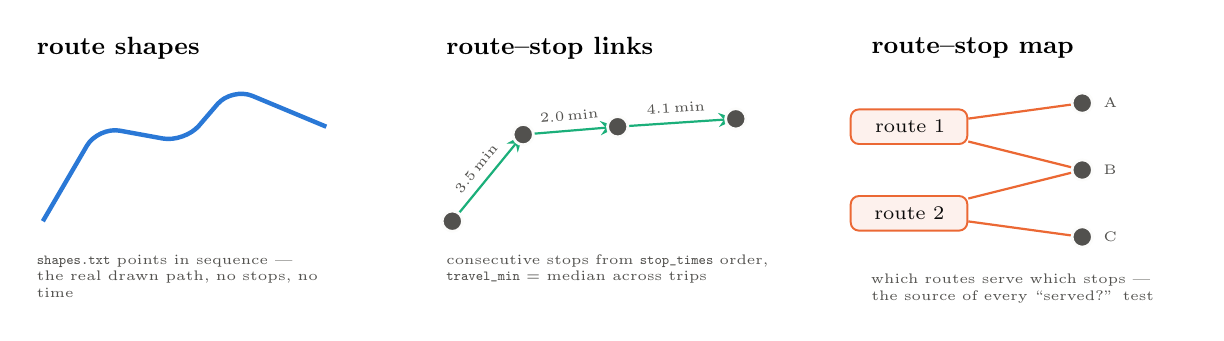
\begin{tikzpicture}[x=1cm,y=1cm]
    % shapes
    \begin{scope}[xshift=0cm]
      \node[font=\small\bfseries, anchor=west] at (0,2.2) {route shapes};
      \draw[cBlue, line width=1.6pt, rounded corners=8pt] (0.2,0) -- (0.9,1.2) -- (2.0,1.0) -- (2.6,1.7) -- (3.8,1.2);
      \node[lbl, anchor=north west, text width=4cm] at (0,-0.3) {\code{shapes.txt} points in sequence ---\\the real drawn path, no stops, no time};
    \end{scope}
    % links
    \begin{scope}[xshift=5.2cm]
      \node[font=\small\bfseries, anchor=west] at (0,2.2) {route--stop links};
      \foreach \a/\b/\t in {{(0.2,0)}/{(1.1,1.1)}/3.5, {(1.1,1.1)}/{(2.3,1.2)}/2.0, {(2.3,1.2)}/{(3.8,1.3)}/4.1}{
        \draw[arr, cAqua] \a -- node[lbl, above, sloped] {\t\,min} \b;}
      \foreach \p in {(0.2,0),(1.1,1.1),(2.3,1.2),(3.8,1.3)} \node[stop=cInkTwo] at \p {};
      \node[lbl, anchor=north west, text width=4.3cm] at (0,-0.3) {consecutive stops from \code{stop_times} order,\\\code{travel_min} = median across trips};
    \end{scope}
    % map
    \begin{scope}[xshift=10.6cm]
      \node[font=\small\bfseries, anchor=west] at (0,2.2) {route--stop map};
      \node[box=cOrange, text width=1.2cm] (r1) at (0.6,1.2) {route 1};
      \node[box=cOrange, text width=1.2cm] (r2) at (0.6,0.1) {route 2};
      \node[stop=cInkTwo, label={[lbl]right:A}] (a) at (2.8,1.5) {};
      \node[stop=cInkTwo, label={[lbl]right:B}] (b) at (2.8,0.65) {};
      \node[stop=cInkTwo, label={[lbl]right:C}] (c) at (2.8,-0.2) {};
      \draw[cOrange, line width=0.8pt] (r1) -- (a); \draw[cOrange, line width=0.8pt] (r1) -- (b);
      \draw[cOrange, line width=0.8pt] (r2) -- (b); \draw[cOrange, line width=0.8pt] (r2) -- (c);
      \node[lbl, anchor=north west, text width=4cm] at (0,-0.55) {which routes serve which stops ---\\the source of every ``served?'' test};
    \end{scope}
  \end{tikzpicture}
  \vskip0.35cm
\begin{lstlisting}[style=algo]
for each trip, ordered by numeric stop_sequence, then stop_id:
    keep one stop per stop_sequence                  # mdb lists light-rail aliases under one number
    seg_s = next departure - this departure          # negative -> NULL (broken sequence)
group by (route, direction, stop, next_stop):
    travel_min = round(median(seg_s) / 60, 1)       n_obs = count of non-NULL seg_s
\end{lstlisting}
\end{frame}

% ============================================================================
\begin{frame}{\step{cPTwo}{9}Can we trust each in-vehicle time?}
  \framesubtitle{Times are kept as published; \code{time_quality} says how much to trust them}
  \begin{columns}[T]
    \column{0.55\textwidth}
    \scriptsize
    \renewcommand{\arraystretch}{1.35}
    \begin{tabularx}{\linewidth}{@{}l >{\raggedright\arraybackslash}X r@{}}
      \hline
      \textbf{Label} & \textbf{Rule} & \textbf{Arcs} \\ \hline
      \code{ok} & none of the below & 24,013 \\
      \code{too_fast} & straight line between the stops $>$ 80\,km/h (the real path is longer) & 18 \\
      \code{too_slow} & route direction: shape km / median trip minutes $<$ 5\,km/h & 4 \\
      \code{zero} & 0\,s between two stops & 1 \\
      \code{untimed} & no time & 0 \\ \hline
    \end{tabularx}
    \vskip0.2cm
    \muted{On the station network's 24,036 \code{in_vehicle} arcs; also on every timetable connection.}
    \column{0.42\textwidth}
    \begin{alertblock}{What the labels caught}
      \scriptsize
      \textbf{zig-zag:} mdb \code{MT_L1}/\code{MT_L2} list each station twice (\code{MT-L1_xx},
      \code{TL_0001_00xx}, 0\,m) under one \code{stop_sequence}: 30 fake 0-minute arcs, now gone.\\[3pt]
      \textbf{placeholders:} every T16B branch is scheduled at 70\,min whatever its length;
      the 3\,km branches run at $\approx$3\,km/h.\\[3pt]
      \textbf{real:} \code{T09-O} takes 110\,min between two stops 150\,m apart --- a 26.6\,km loop.
    \end{alertblock}
  \end{columns}
\end{frame}

% ============================================================================
\begin{frame}{\step{cPTwo}{10}Find proximity pairs}
  \framesubtitle{Every pair of stops closer than \code{--proximity-m}, across all feeds}
  \begin{columns}[c]
    \column{0.42\textwidth}
    \centering
    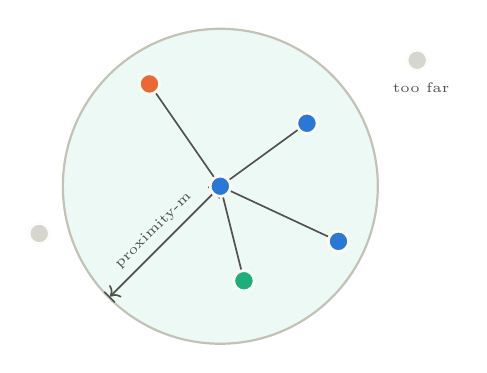
\begin{tikzpicture}[x=1cm,y=1cm]
      \fill[cAqua!8] (0,0) circle (2.0);
      \draw[cBase, line width=0.8pt] (0,0) circle (2.0);
      \draw[cInkTwo, |<->|, line width=0.6pt] (0,0) -- node[lbl, above, sloped] {proximity-m} (-1.414,-1.414);
      \node[stop=cBlue] (s) at (0,0) {};
      \foreach \p/\c in {(1.1,0.8)/cBlue, (-0.9,1.3)/cOrange, (1.5,-0.7)/cBlue, (0.3,-1.2)/cAqua}{
        \node[stop=\c] (n) at \p {}; \draw[cInkTwo, line width=0.6pt] (s) -- (n);}
      \node[stop=cContext] at (2.5,1.6) {};
      \node[stop=cContext] at (-2.3,-0.6) {};
      \node[lbl] at (2.55,1.25) {too far};
    \end{tikzpicture}
    \column{0.56\textwidth}
    \small
    $\mathit{pairs} = \{\,(a,b) : \mathit{uid}_a < \mathit{uid}_b,\ \mathit{dist}(a,b) \le r\,\}$
    \vskip0.3cm
    \renewcommand{\arraystretch}{1.35}
    \scriptsize
    \begin{tabularx}{\linewidth}{@{}l>{\raggedright\arraybackslash}X@{}}
      \hline
      \textbf{Path} & \textbf{How} \\ \hline
      PostGIS & \code{ST_DWithin} on \code{geography}, GiST-indexed, on the \code{stops} table, filtered by feed \\
      Local (\code{--dry-run}) & project to UTM, spatial-index join with \code{dwithin} \\ \hline
    \end{tabularx}
    \vskip0.3cm
    \begin{alertblock}{A trap dry runs cannot catch}
      \scriptsize The database path filters by feed id. Stops-only feeds must be in that list, or their rows
      match nothing --- while the local path ignores the list and looks perfect.
    \end{alertblock}
  \end{columns}
\end{frame}

% ============================================================================
\begin{frame}{\step{cPTwo}{11}Deduplicate stations: two rules, different evidence}
  \begin{columns}[T]
    \column{0.6\textwidth}
    \centering
    \resizebox{\linewidth}{!}{%
    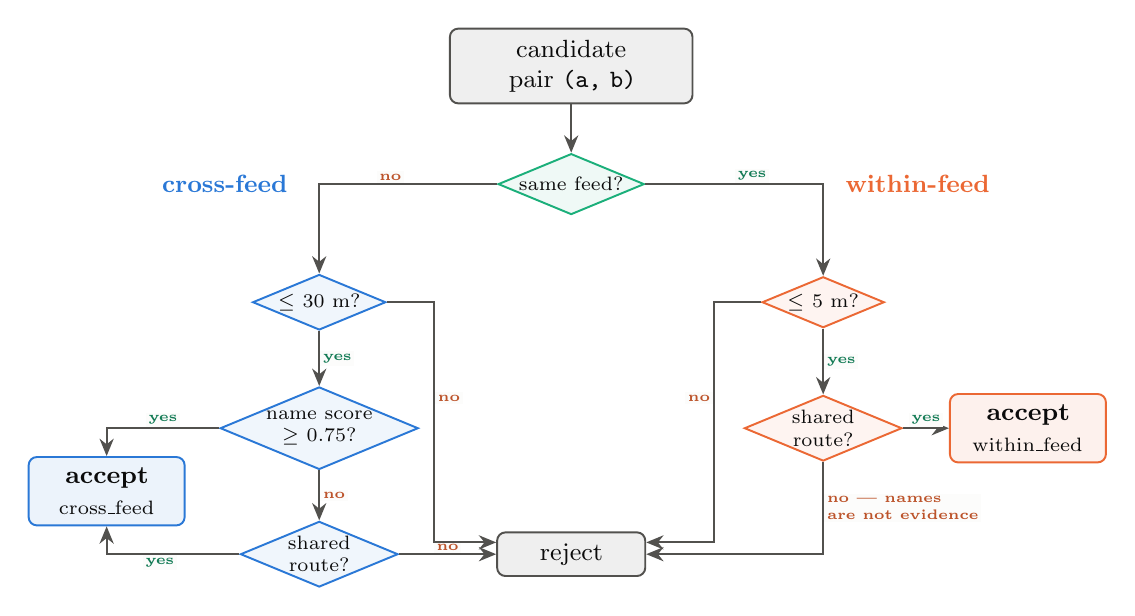
\begin{tikzpicture}[x=1cm,y=1cm, dec/.append style={font=\scriptsize}]
      \node[box, text width=2.8cm, font=\small] (c) at (3.2,0) {candidate pair \code{(a, b)}};
      \node[dec=cPTwo] (sf) at (3.2,-1.5) {same feed?};
      \node[font=\small\bfseries, text=cBlue] at (-1.2,-1.5) {cross-feed};
      \node[font=\small\bfseries, text=cOrange] at (7.6,-1.5) {within-feed};
      % cross-feed
      \node[dec=cBlue] (r30) at (0,-3.0) {$\le$ 30 m?};
      \node[dec=cBlue] (nm) at (0,-4.6) {name score\\$\ge$ 0.75?};
      \node[dec=cBlue] (sr1) at (0,-6.2) {shared\\route?};
      \node[box=cBlue, text width=1.7cm, font=\small] (acc1) at (-2.7,-5.4) {\textbf{accept}\\ \scriptsize cross\_feed};
      % within-feed
      \node[dec=cOrange] (r50) at (6.4,-3.0) {$\le$ 5 m?};
      \node[dec=cOrange] (sr2) at (6.4,-4.6) {shared\\route?};
      \node[box=cOrange, text width=1.7cm, font=\small] (acc2) at (9.0,-4.6) {\textbf{accept}\\ \scriptsize within\_feed};
      \node[box, text width=1.6cm, font=\small] (rej) at (3.2,-6.2) {reject};
      \draw[arr] (c) -- (sf);
      \draw[arr] (sf) -| node[no, pos=0.3, above] {no} (r30);
      \draw[arr] (sf) -| node[yes, pos=0.3, above] {yes} (r50);
      \draw[arr] (r30) -- node[yes, right] {yes} (nm);
      \draw[arr] (nm) -| node[yes, pos=0.25, above] {yes} (acc1);
      \draw[arr] (nm) -- node[no, right] {no} (sr1);
      \draw[arr] (sr1) -| node[yes, pos=0.3, below] {yes} (acc1);
      \draw[arr] (sr1) -- node[no, above] {no} (rej);
      \draw[arr] (r30.east) -- ++(0.6,0) |- node[no, pos=0.2, right] {no} ([yshift=0.15cm]rej.west);
      \draw[arr] (r50) -- node[yes, right] {yes} (sr2);
      \draw[arr] (sr2) -- node[yes, above] {yes} (acc2);
      \draw[arr] (sr2) |- node[no, pos=0.25, right, align=left] {no --- names\\are not evidence} (rej);
      \draw[arr] (r50.west) -- ++(-0.6,0) |- node[no, pos=0.2, left] {no} ([yshift=0.15cm]rej.east);
    \end{tikzpicture}}
    \column{0.38\textwidth}
    \begin{block}{Why names can't merge a within-feed pair}
      \scriptsize Two genuinely different stops of one feed can share a name --- a long avenue, a plaza.
      Two stops of the \textbf{same route} within tens of metres are almost surely one station recorded
      twice. 5\,m, not 50\,m: the same route's stop across the street is 20--40\,m away.
    \end{block}
    \vskip0.2cm
    \begin{exampleblock}{MiBici is never deduplicated}
      \scriptsize Stops-only sources are excluded from both rules: a dock is never an alias of a bus stop.
    \end{exampleblock}
    \vskip0.1cm
    \muted{\scriptsize Accepted pairs form a graph: each connected component is one station.}
  \end{columns}
\end{frame}

% ============================================================================
\begin{frame}[fragile]{\step{cPTwo}{11}The evidence functions}
  \begin{columns}[T]
    \column{0.5\textwidth}
    \textbf{Name similarity}
    \vskip0.15cm
    \centering
    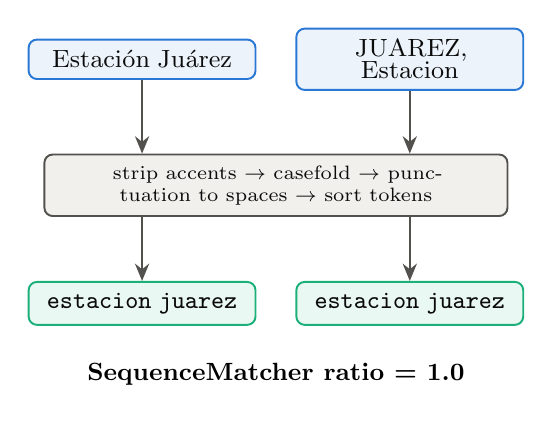
\begin{tikzpicture}[x=1cm,y=1cm]
      \node[box=cBlue, text width=2.6cm] (a) at (0,0) {\small Estación Juárez};
      \node[box=cBlue, text width=2.6cm] (b) at (3.4,0) {\small JUAREZ, Estacion};
      \node[box, text width=5.6cm, fill=cCode] (n) at (1.7,-1.6)
        {\scriptsize strip accents $\rightarrow$ casefold $\rightarrow$ punctuation to spaces $\rightarrow$ sort tokens};
      \node[box=cAqua, text width=2.6cm] (na) at (0,-3.1) {\ttfamily\small estacion juarez};
      \node[box=cAqua, text width=2.6cm] (nb) at (3.4,-3.1) {\ttfamily\small estacion juarez};
      \draw[arr] (a) -- (n.north -| a); \draw[arr] (b) -- (n.north -| b);
      \draw[arr] (n.south -| a) -- (na); \draw[arr] (n.south -| b) -- (nb);
      \node[font=\small\bfseries] at (1.7,-4.0) {SequenceMatcher ratio = 1.0};
    \end{tikzpicture}
    \column{0.48\textwidth}
    \textbf{Shared routes and the audit score}
\begin{lstlisting}[style=algo]
routes(stop)  = { normalize(route_short_name)
                  of routes serving the stop }
shared_routes = | routes(a) & routes(b) |

score = 0.5 * (1 - dist / radius_that_admitted)
      + 0.5 * name_score        # audit only
\end{lstlisting}
    \vskip0.2cm
    \small
    \begin{itemize}
      \item Empty name $\Rightarrow$ \code{name_score = 0}
      \item \code{score} is never a gate --- it only helps review
      \item Every accepted pair records \code{match_kind}, so the two rules stay separately auditable
    \end{itemize}
  \end{columns}
\end{frame}

% ============================================================================
\begin{frame}{\step{cPTwo}{11}The same-feed conflict guard}
  \framesubtitle{Accepted pairs chain into groups --- a group may not hold two far-apart stops of one feed}
  \begin{columns}[c]
    \column{0.5\textwidth}
    \centering
    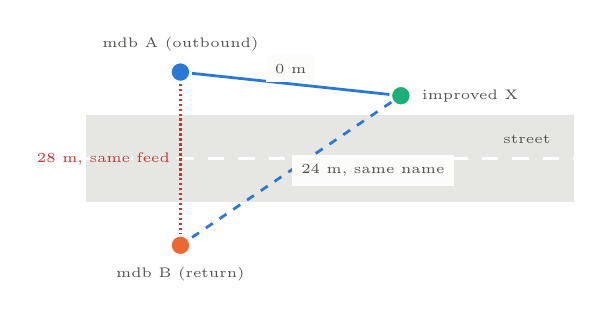
\begin{tikzpicture}[x=1cm,y=1cm]
      \fill[cContext!60] (-0.6,0.95) rectangle (5.6,2.05);
      \draw[white, line width=1.2pt, dash pattern=on 6pt off 5pt] (-0.6,1.5) -- (5.6,1.5);
      \node[lbl] at (5.0,1.75) {street};
      \node[stop=cBlue, label={[lbl]above:{mdb A (outbound)}}] (a) at (0.6,2.6) {};
      \node[stop=cOrange, label={[lbl]below:{mdb B (return)}}] (b) at (0.6,0.4) {};
      \node[stop=cAqua, label={[lbl]right:{improved X}}] (x) at (3.4,2.3) {};
      \draw[cBlue, line width=1pt] (a) -- node[lbl, above, fill=cSurface] {0 m} (x);
      \draw[cBlue, line width=1pt, dashed] (x) -- node[lbl, right, fill=cSurface] {24 m, same name} (b);
      \draw[cRed, line width=0.8pt, densely dotted] (a) -- node[lbl, left, text=cRed] {28 m, same feed} (b);
    \end{tikzpicture}
    \column{0.48\textwidth}
    \small
    \begin{itemize}
      \item Cross-feed pairs alone can chain A $\sim$ X $\sim$ B: two opposite platforms of one feed in one ``station''.
      \item Greedy union, closest pairs first: a pair is \textbf{rejected} if it would join two stops of the
            same feed more than 5\,m apart.
      \item Rejected pairs go to \code{stop_equivalences_rejected.csv}; the stops stay neighbours (walk links).
    \end{itemize}
    \vskip0.2cm
    \begin{columns}[T]
      \column{0.48\linewidth}\centering\stat{772}{pairs rejected}{cOrange}
      \column{0.48\linewidth}\centering\stat{7.5\,m}{widest station}{cAqua}
    \end{columns}
  \end{columns}
\end{frame}

% ============================================================================
\begin{frame}{\step{cPTwo}{11}Dedupe measured: 2,812 accepted pairs}
  \begin{columns}[c]
    \column{0.6\textwidth}
    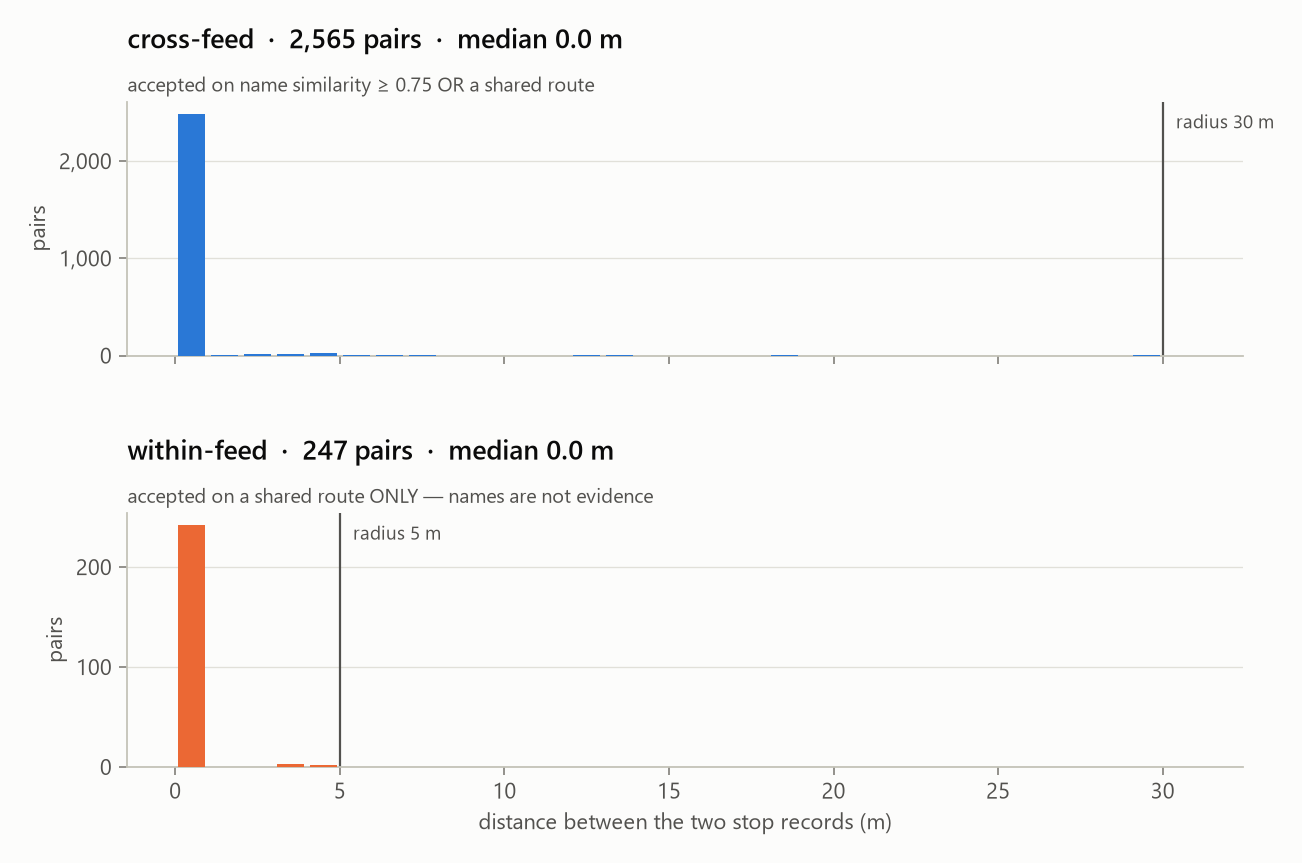
\includegraphics[width=\linewidth]{r2_dedupe_distances.png}
    \column{0.38\textwidth}
    \small
    \begin{itemize}
      \item \textbf{Cross-feed: 2,565 pairs, median 0.0\,m.} Most are exact coordinate copies --- the two
            feeds share a stop inventory.
      \item \textbf{Within-feed: 247 pairs, all $\le$ 4.6\,m.} One station recorded twice (\code{SITEUR_*} and
            \code{ST_*} light-rail ids).
      \item \textbf{1,604 groups}; 12,768 served records $\rightarrow$ \textbf{10,203 stations}.
            Median group span 0\,m, widest 7.5\,m.
    \end{itemize}
  \end{columns}
\end{frame}

% ============================================================================
\begin{frame}{\step{cPTwo}{11}One real place, many records}
  \centering
  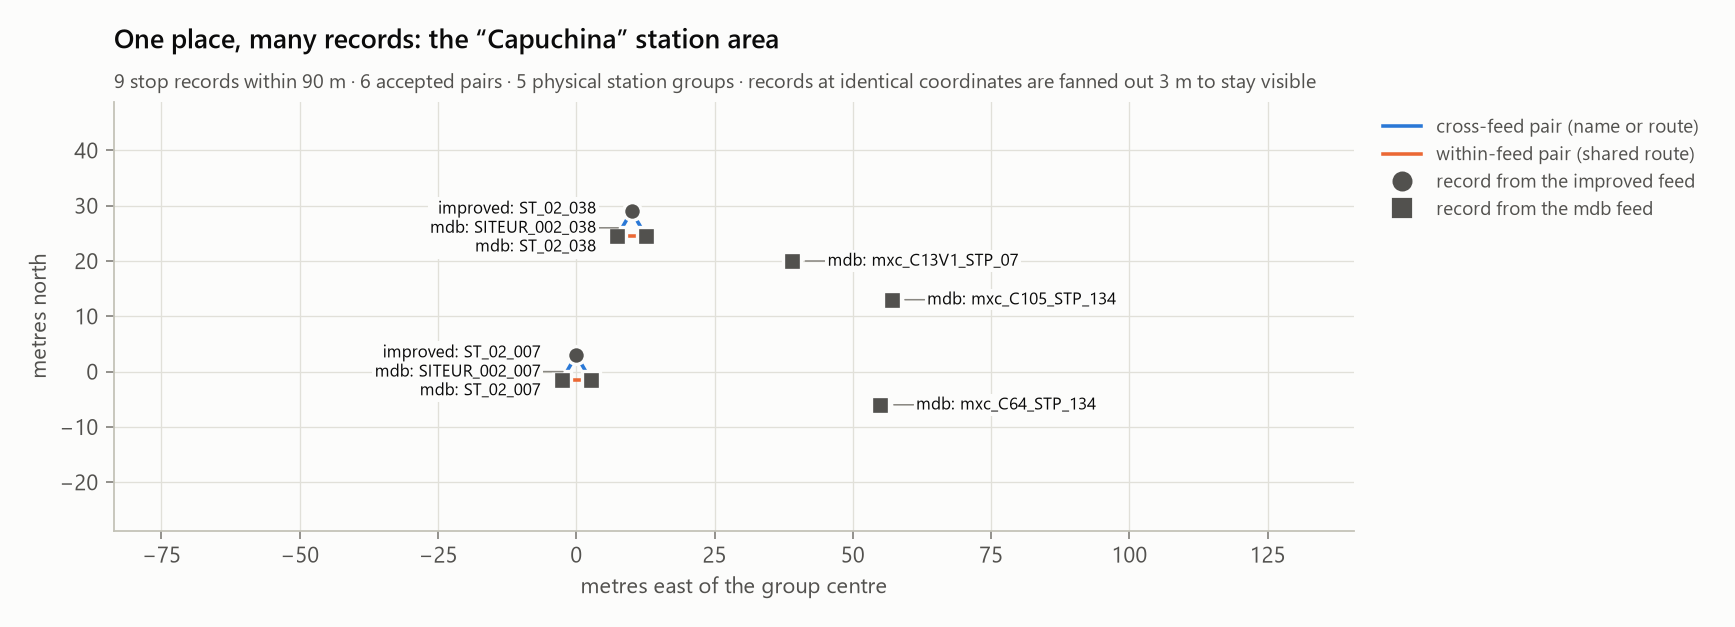
\includegraphics[width=0.9\textwidth]{r3_duplicate_cluster_map.png}
  \vskip0.05cm
  \begin{columns}[T]
    \column{0.47\textwidth}
    \scriptsize\textbf{Both rules at once.} Around one SiTren station, 9 records form 5 groups:
    \code{ST_02_007} matches across feeds (blue); \code{SITEUR_*} and \code{ST_*} match inside one feed
    on a shared route (orange). Nearby bus stops stay separate stations.
    \column{0.49\textwidth}
    \begin{exampleblock}{Opposite platforms stay apart}
      \scriptsize \code{ST_02_007} and \code{ST_02_038} are the two directions of one line, 26\,m apart.
      With the 5\,m rule and the conflict guard they are two stations joined by a walk link --- no free
      U-turn when routing.
    \end{exampleblock}
  \end{columns}
\end{frame}

% ============================================================================
\begin{frame}{\step{cPTwo}{11b}One source per line}
  \framesubtitle{A line published by two feeds would run twice in a timetable: double frequency, half the wait}
  \begin{columns}[c]
    \column{0.58\textwidth}
    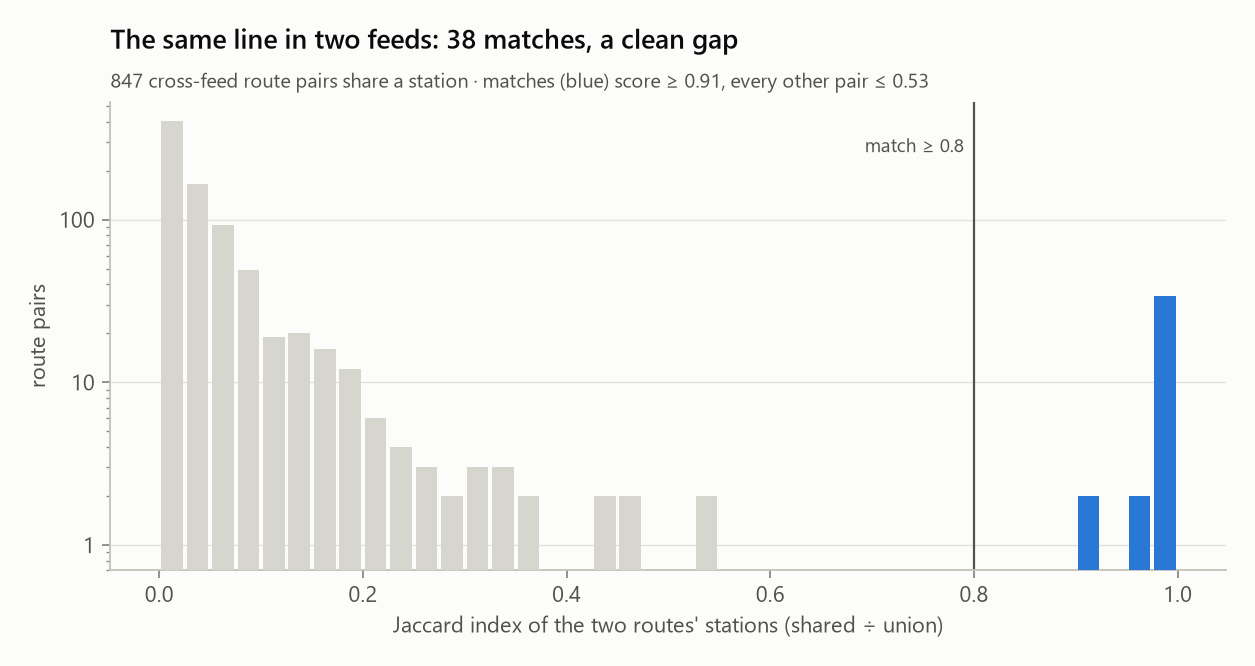
\includegraphics[width=\linewidth]{r11_route_jaccard.png}
    \column{0.4\textwidth}
    \scriptsize
    \begin{block}{Rule}
      stations(route) = its stops mapped to dedupe groups\\
      match if Jaccard $\ge$ 0.8, best first, one-to-one\\
      keep the feed with the later calendar
    \end{block}
    \begin{itemize}
      \item Ids and short names can't decide: \code{2215-C98} vs \code{C98}; \code{L1} is both Mi Tren and SiTren
      \item \textbf{38 lines} in both feeds, all kept from mdb; improved keeps \code{MP-A05-2}, \code{ST_L1B}
      \item mdb lists every SiTren trip twice (\code{SITEUR_T_xx}, \code{ST_xx}): 8 dropped
      \item Routing inputs only; \code{routes.csv} keeps both with \code{duplicate_of}
    \end{itemize}
  \end{columns}
\end{frame}

% ============================================================================
\begin{frame}{\step{cPTwo}{12}Build route connectivity}
  \framesubtitle{Four ways two routes can meet --- the strongest evidence names the edge}
  \begin{columns}[c]
    \column{0.55\textwidth}
    \centering
    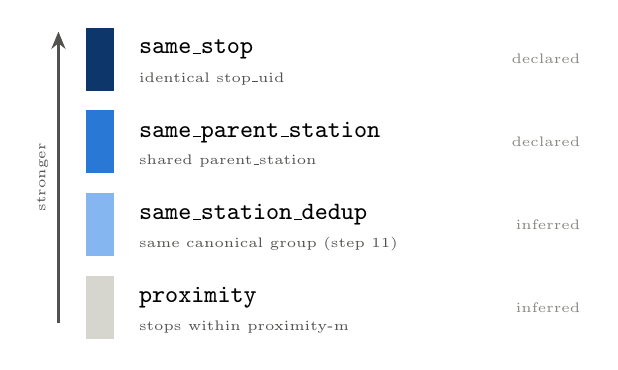
\begin{tikzpicture}[x=1cm,y=1cm]
      \foreach \y/\col/\name/\rule/\kind in {
        3/cRampDark/same\_stop/identical stop\_uid/declared,
        2/cBlue/same\_parent\_station/shared parent\_station/declared,
        1/cRampLight/same\_station\_dedup/same canonical group (step 11)/inferred,
        0/cContext/proximity/stops within proximity-m/inferred}
      {
        \fill[\col] (0,\y*1.05) rectangle ++(0.35,0.8);
        \node[anchor=west, font=\small\bfseries\ttfamily] at (0.55,\y*1.05+0.52) {\name};
        \node[anchor=west, lbl] at (0.55,\y*1.05+0.15) {\rule};
        \node[anchor=east, font=\tiny, text=cMuted] at (6.4,\y*1.05+0.4) {\kind};
      }
      \draw[arr, cInkTwo] (-0.35,0.2) -- node[lbl, left, rotate=90, anchor=south] {stronger} (-0.35,3.9);
    \end{tikzpicture}
    \column{0.43\textwidth}
    \small
    \begin{enumerate}\scriptsize
      \item For each rule: \code{route_stops} $\bowtie$ relation $\bowtie$ \code{route_stops}
      \item Drop self-pairs; order so \code{route_a < route_b}
      \item Outer-merge the four sets on the route pair
      \item Label with the \textbf{strongest} rule that produced it
      \item \code{min_stop_distance_m} = 0 for \code{same_stop}, else closest proximity pair
    \end{enumerate}
    \vskip0.3cm
    \begin{block}{Declared vs inferred}
      \scriptsize \code{same_station_dedup} stays separate from \code{same_parent_station}: one is inferred by
      the pipeline, the other declared by the operator.
    \end{block}
    \vskip0.1cm
    \muted{\scriptsize 249 routes, 7,902 pairs, 1 component. \code{route_connection_stops.csv} lists
    \emph{where}: every route pair and stop pair behind an edge.}
  \end{columns}
\end{frame}

% ============================================================================
\begin{frame}{\step{cPTwo}{13}Walk on real OSM streets}
  \framesubtitle{Straight-line distance understates walking --- route it on the street network}
  \centering
  \resizebox{\textwidth}{!}{%
  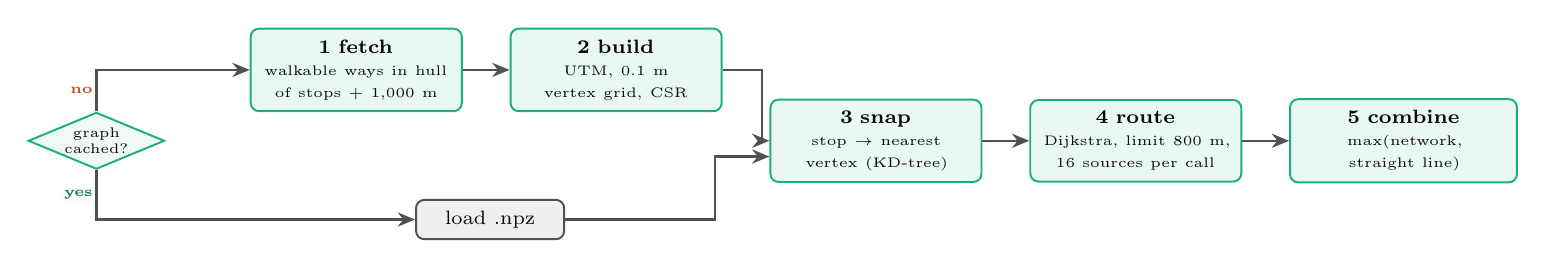
\begin{tikzpicture}[x=1cm,y=1cm]
    \node[dec=cPTwo] (k) at (0,0) {graph\\cached?};
    \node[box=cPTwo, text width=2.4cm] (f) at (3.3,0.9) {\textbf{1 fetch}\\ \tiny walkable ways in hull of stops + 1,000 m};
    \node[box=cPTwo, text width=2.4cm] (b) at (6.6,0.9) {\textbf{2 build}\\ \tiny UTM, 0.1 m vertex grid, CSR};
    \node[box, text width=1.6cm] (l) at (5.0,-1.0) {load .npz};
    \node[box=cPTwo, text width=2.4cm] (s) at (9.9,0) {\textbf{3 snap}\\ \tiny stop $\rightarrow$ nearest vertex (KD-tree)};
    \node[box=cPTwo, text width=2.4cm] (r) at (13.2,0) {\textbf{4 route}\\ \tiny Dijkstra, limit 800 m, 16 sources per call};
    \node[box=cAqua, text width=2.6cm] (c) at (16.6,0) {\textbf{5 combine}\\ \tiny max(network, straight line)};
    \draw[arr] (k) |- node[no, pos=0.25, left] {no} (f);
    \draw[arr] (f) -- (b);
    \draw[arr] (b.east) -- ++(0.5,0) |- (s.west);
    \draw[arr] (k) |- node[yes, pos=0.25, left] {yes} (l);
    \draw[arr] (l.east) -- ++(1.9,0) |- ([yshift=-0.2cm]s.west);
    \draw[arr] (s) -- (r); \draw[arr] (r) -- (c);
  \end{tikzpicture}}
  \vskip0.4cm
  \begin{columns}[T]
    \column{0.32\textwidth}
    \begin{block}{Fetch \& build}
      \scriptsize \code{highway} ways except motorway, motorway\_link, proposed, construction. Endpoints snap
      to a 10\,cm grid; ways connect only where they \textbf{share a coordinate} --- bridges stay unconnected.
    \end{block}
    \column{0.32\textwidth}
    \begin{block}{Snap \& route}
      \scriptsize Nearest \emph{vertex}, not nearest edge point. Snap $>$ 200\,m is labelled \code{unsnapped}.
      Each Dijkstra call allocates 16 $\times$ 512,420 floats $\approx$ 66\,MB.
    \end{block}
    \column{0.32\textwidth}
    \begin{block}{Cache key}
      \scriptsize Feed ids, hull buffer, OSM table and column, excluded highways, CRS --- plus OSM row count,
      max \code{osm_id} and the stops' latest load time.
    \end{block}
  \end{columns}
\end{frame}

% ============================================================================
\begin{frame}{\step{cPTwo}{13}Inside the walk graph}
  \framesubtitle{How one pair of stops gets a walking distance}
  \begin{columns}[c]
  \column{0.6\textwidth}
  \centering
  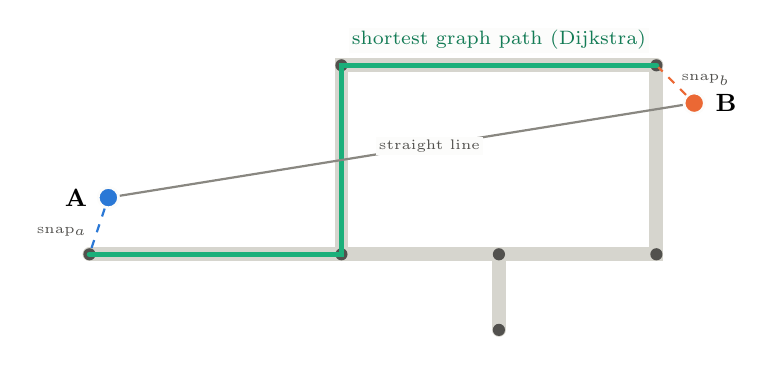
\begin{tikzpicture}[x=0.8cm,y=0.8cm]
    % streets
    \draw[cContext, line width=5pt, line cap=round] (0,0) -- (4,0) -- (4,3) -- (9,3);
    \draw[cContext, line width=5pt, line cap=round] (4,0) -- (9,0) -- (9,3);
    \draw[cContext, line width=5pt, line cap=round] (6.5,0) -- (6.5,-1.2);
    \foreach \p in {(0,0),(4,0),(4,3),(9,3),(9,0),(6.5,0),(6.5,-1.2)} \fill[cInkTwo] \p circle (2.2pt);
    % stops
    \node[stop=cBlue, label={[font=\small\bfseries]left:A}] (A) at (0.3,0.9) {};
    \node[stop=cOrange, label={[font=\small\bfseries]right:B}] (B) at (9.6,2.4) {};
    \draw[cBlue, dashed, line width=0.8pt] (A) -- (0,0) node[pos=0.5, lbl, left] {snap$_a$};
    \draw[cOrange, dashed, line width=0.8pt] (B) -- (9,3) node[pos=0.5, lbl, right] {snap$_b$};
    % path
    \draw[cAqua, line width=2pt, line cap=round] (0,0) -- (4,0) -- (4,3) -- (9,3);
    \node[font=\scriptsize, text=cAqua!70!black, fill=cSurface, inner sep=1pt] at (6.5,3.4) {shortest graph path (Dijkstra)};
    % straight line
    \draw[cMuted, line width=0.8pt] (A) -- (B) node[pos=0.55, lbl, fill=cSurface, inner sep=1pt] {straight line};
  \end{tikzpicture}
  \column{0.38\textwidth}
    \begin{block}{Combine}
      \small $\mathit{network} = \mathit{path} + \mathit{snap}_a + \mathit{snap}_b$\\[3pt]
      $\mathit{distance} = \max(\mathit{network},\ \mathit{straight\ line})$\\[3pt]
      \scriptsize no path within 800\,m $\Rightarrow$ keep the straight line, \code{walk_source = straight_line}
    \end{block}
    \vskip0.3cm
    \small Applied \textbf{after} step 12 (connectivity stays geodesic) and \textbf{before} step 14 (walking
    minutes use real streets).
  \end{columns}
\end{frame}

% ============================================================================
\begin{frame}{\step{cPTwo}{13}How much longer is the real walk?}
  \begin{columns}[c]
    \column{0.64\textwidth}
    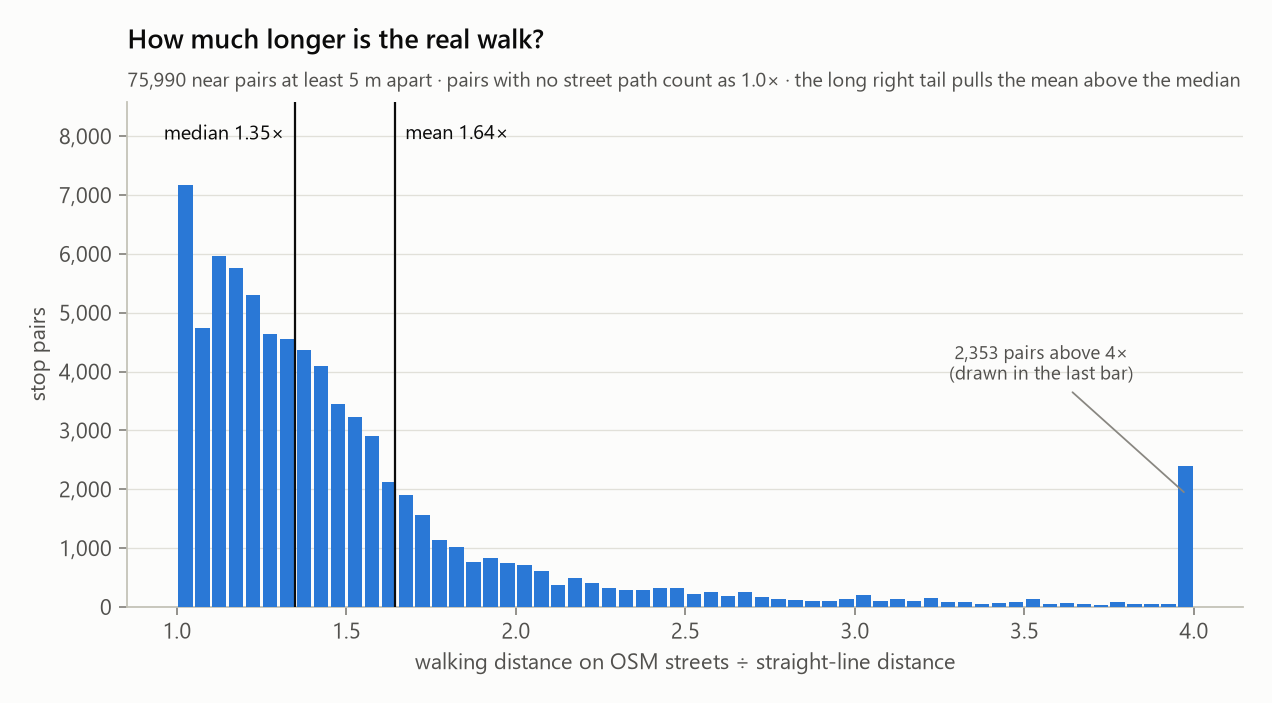
\includegraphics[width=\linewidth]{r5_detour_distribution.png}
    \column{0.34\textwidth}
    \centering
    \stat{1.35$\times$}{median walk / straight line}{cAqua}
    \vskip0.3cm
    \raggedright\small
    \begin{itemize}\scriptsize
      \item 75,990 pairs at least 5\,m apart; 74,689 of 77,706 routed on streets
      \item Mean 1.64$\times$: a long tail of big detours
      \item 2,353 pairs above 4$\times$
    \end{itemize}
    \begin{alertblock}{Use the median}
      \scriptsize The run log's ``73\,\% detour'' (1.73$\times$) averages routed pairs only, including
      near-co-located stops whose tiny straight line inflates the ratio.
    \end{alertblock}
  \end{columns}
\end{frame}

% ============================================================================
\begin{frame}{\step{cPTwo}{14}Near stations and same-line stations}
  \framesubtitle{Two relations per stop, with deliberately different inclusion rules}
  \begin{columns}[T]
    \column{0.49\textwidth}
    \centering
    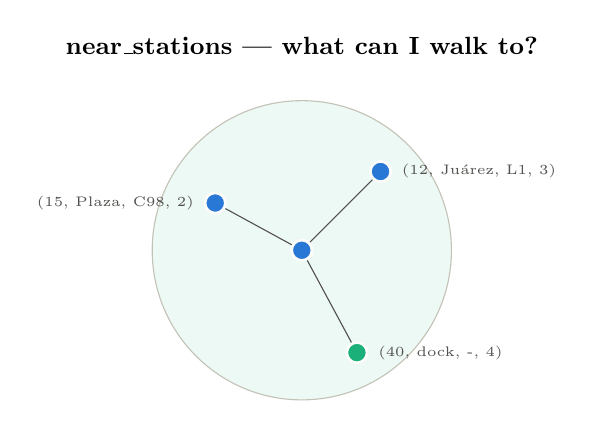
\begin{tikzpicture}[x=1cm,y=1cm]
      \node[font=\small\bfseries] at (0,2.6) {near\_stations --- what can I walk to?};
      \fill[cAqua!8] (0,0) circle (1.9); \draw[cBase] (0,0) circle (1.9);
      \node[stop=cBlue] (s) at (0,0) {};
      \node[stop=cBlue, label={[lbl]right:{(12, Juárez, L1, 3)}}] (a) at (1.0,1.0) {};
      \node[stop=cBlue, label={[lbl]left:{(15, Plaza, C98, 2)}}] (b) at (-1.1,0.6) {};
      \node[stop=cAqua, label={[lbl]right:{(40, dock, -, 4)}}] (c) at (0.7,-1.3) {};
      \draw[cInkTwo] (s) -- (a); \draw[cInkTwo] (s) -- (b); \draw[cInkTwo] (s) -- (c);
    \end{tikzpicture}
    \vskip0.1cm
    \scriptsize
    \begin{itemize}
      \item Distance only, any line
      \item $\mathit{minutes} = \max(1,\ \mathrm{round}(\mathit{metres}/83))$
      \item Unserved neighbour listed with line \code{-}
    \end{itemize}
    \column{0.49\textwidth}
    \centering
    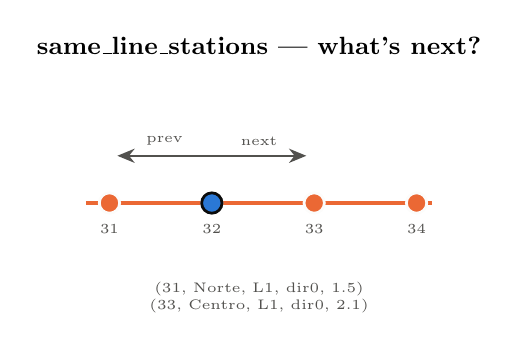
\begin{tikzpicture}[x=1cm,y=1cm]
      \node[font=\small\bfseries] at (1.9,2.6) {same\_line\_stations --- what's next?};
      \draw[cOrange, line width=1.5pt] (-0.3,0.6) -- (4.1,0.6);
      \foreach \x/\n in {0/31,1.3/32,2.6/33,3.9/34} \node[stop=cOrange, label={[lbl]below:\n}] at (\x,0.6) {};
      \node[stop=cBlue, draw=cInk, line width=1pt] at (1.3,0.6) {};
      \draw[arr, cInkTwo] (1.3,1.2) -- node[lbl, above] {prev} (0.1,1.2);
      \draw[arr, cInkTwo] (1.3,1.2) -- node[lbl, above] {next} (2.5,1.2);
      \node[lbl, text width=4.4cm, align=center] at (1.9,-0.6) {(31, Norte, L1, dir0, 1.5)\quad(33, Centro, L1, dir0, 2.1)};
    \end{tikzpicture}
    \vskip0.1cm
    \scriptsize
    \begin{itemize}
      \item Sequence only, no distance limit
      \item Minutes = scheduled \code{travel_min}, else haversine at 25\,km/h
      \item Previous \emph{and} next stop, per line and direction
    \end{itemize}
  \end{columns}
  \vskip0.05cm
  \muted{\tiny \code{ID} = 1..N in row order, referenced by every tuple; \code{stop_uid} is the cross-run key.}
\end{frame}

% ============================================================================
\begin{frame}{\step{cPTwo}{14}near\_stations for one real MiBici dock}
  \begin{columns}[c]
    \column{0.58\textwidth}
    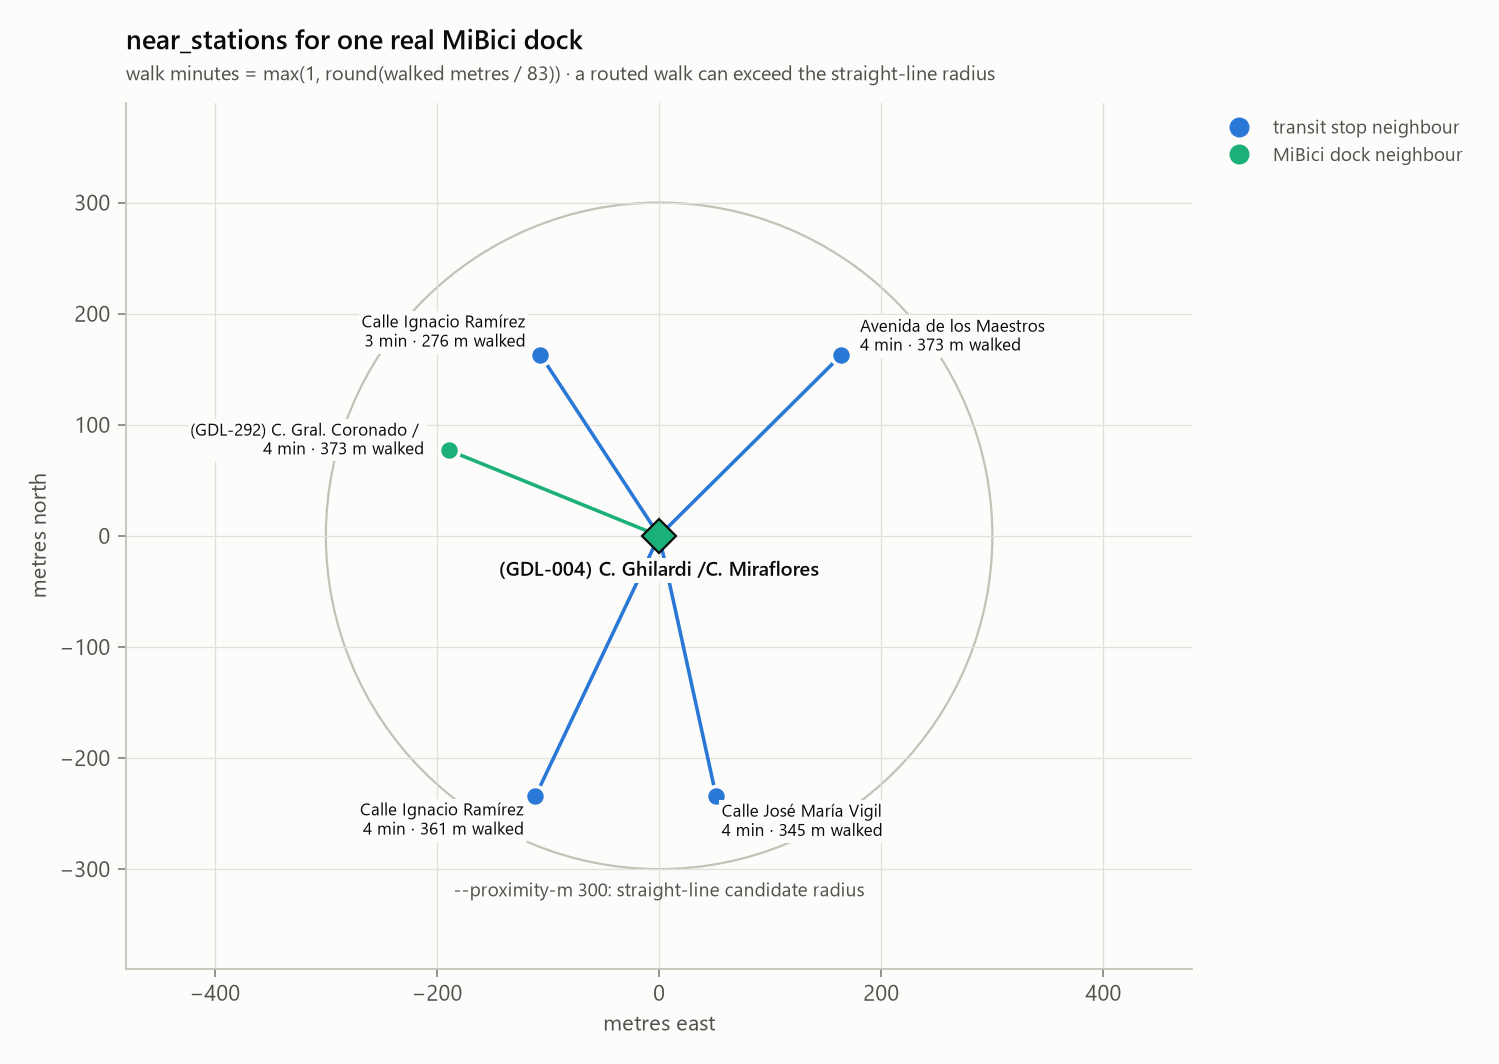
\includegraphics[width=\linewidth]{r4_near_stations_example.png}
    \column{0.4\textwidth}
    \small
    \begin{itemize}
      \item Four transit stops and one dock, 3--4 minutes' walk
      \item Candidates are chosen by \textbf{straight line} (the circle)\ldots
      \item \ldots but the reported distance is the \textbf{street walk} from step 13
    \end{itemize}
    \vskip0.3cm
    \begin{block}{So a walk can exceed the radius}
      \scriptsize Four neighbours are 345--373\,m \emph{walked} while sitting inside the 300\,m
      straight-line circle.
    \end{block}
  \end{columns}
\end{frame}

% ============================================================================
\begin{frame}{\step{cPTwo}{15}The quality sidecar: how each value was obtained}
  \framesubtitle{A measured 4 minutes and an estimated 4 minutes look identical --- the sidecar tells them apart}
  \footnotesize
  \renewcommand{\arraystretch}{1.3}
  \begin{tabularx}{\textwidth}{@{}l >{\raggedright\arraybackslash}p{4.6cm} >{\raggedright\arraybackslash}X@{}}
    \hline
    \textbf{Column} & \textbf{Values} & \textbf{Rule} \\ \hline
    \code{walk_source} & network, straight\_line, mixed, unsnapped, none &
      label shared by the stop's neighbours; \code{mixed} if they disagree; \code{unsnapped} if snap $>$ 200\,m \\
    \code{travel_source} & observed, estimated, mixed, none & scheduled \code{travel_min} vs the 25\,km/h fallback \\
    \code{travel_n_obs} & integer & minimum trips behind the stop's medians --- the weakest evidence \\
    \code{coord_confidence} & 0.812, needs\_review, no\_match, unavailable & from \code{stop_osm_matches} (step 20) \\
    \code{station_dedup} & canonical\_uid or empty & the stop's dedupe group --- \textbf{use it to count stations} \\ \hline
  \end{tabularx}
  \vskip0.2cm
  \muted{\scriptsize Same rows and \code{ID}s as \code{near_stations.csv}; the main file's format never changes because of it.}
\end{frame}

% ============================================================================
\begin{frame}[fragile]{\step{cPTwo}{16}The station network: a routable graph of places}
  \begin{columns}[c]
    \column{0.5\textwidth}
    \centering
    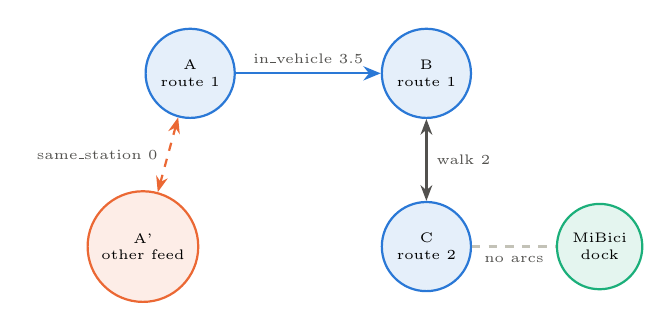
\begin{tikzpicture}[x=1cm,y=1cm, pl/.style={circle, draw=#1, fill=#1!12, line width=0.8pt,
        minimum size=0.95cm, font=\tiny, align=center}]
      \node[pl=cBlue] (a) at (0,2) {A\\route 1};
      \node[pl=cBlue] (b) at (3,2) {B\\route 1};
      \node[pl=cBlue] (c) at (3,-0.2) {C\\route 2};
      \node[pl=cOrange] (a2) at (-0.6,-0.2) {A'\\other feed};
      \node[pl=cAqua] (d) at (5.2,-0.2) {MiBici\\dock};
      \draw[arr, cBlue] (a) -- node[lbl, above] {in\_vehicle 3.5} (b);
      \draw[{Stealth[length=2mm]}-{Stealth[length=2mm]}, line width=0.8pt, cInkTwo] (b) -- node[lbl, right] {walk 2} (c);
      \draw[{Stealth[length=2mm]}-{Stealth[length=2mm]}, line width=0.8pt, cOrange, dashed] (a) -- node[lbl, left] {same\_station 0} (a2);
      \draw[line width=0.8pt, cBase, dashed] (c) -- node[lbl, below] {no arcs} (d);
    \end{tikzpicture}
\begin{lstlisting}[style=algo]
nx.shortest_path(G, a, b, weight="time_min")
\end{lstlisting}
    \column{0.48\textwidth}
    \scriptsize
    \renewcommand{\arraystretch}{1.35}
    \begin{tabularx}{\linewidth}{@{}l l>{\raggedright\arraybackslash}X@{}}
      \hline
      \textbf{Edge} & \textbf{time\_min} & \textbf{Built from} \\ \hline
      \code{in_vehicle} & \code{travel_min} & each route--stop link, one directed arc \\
      \code{walk} & $\max(1, \mathrm{round}(m/83))$ & each proximity pair, two arcs \\
      \code{same_station} & 0 & each dedupe pair, two arcs \\ \hline
    \end{tabularx}
    \vskip0.3cm
    \small Riding, walking and transferring in one graph. MiBici docks are \textbf{unlinked nodes}: they
    were stepping stones that let walks chain past the 300\,m limit.
    \vskip0.25cm
    \scriptsize
    \begin{tabular}{@{}l r@{}}
      \code{in_vehicle} arcs (route-dedupe winners) & 24,036 \\
      \code{walk} arcs (72,286 pairs) & 144,572 \\
      \code{same_station} arcs (2,812 pairs) & 5,624 \\
      weak components among 12,284 transit stops & \textbf{1} \\
    \end{tabular}
  \end{columns}
\end{frame}

% ============================================================================
\begin{frame}{\step{cPTwo}{16}Many arcs never change a shortest time}
  \framesubtitle{Reported on every run; \code{--prune-station-network} drops them (off by default)}
  \begin{columns}[c]
    \column{0.45\textwidth}
    \centering
    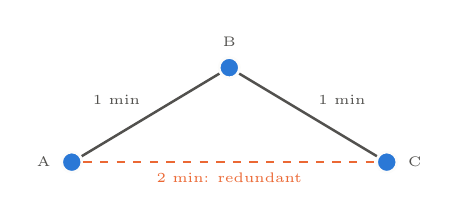
\begin{tikzpicture}[x=1cm,y=1cm]
      \node[stop=cBlue, label={[lbl]left:A}] (a) at (0,0) {};
      \node[stop=cBlue, label={[lbl]above:B}] (b) at (2,1.2) {};
      \node[stop=cBlue, label={[lbl]right:C}] (c) at (4,0) {};
      \draw[cInkTwo, line width=0.9pt] (a) -- node[lbl, above left] {1 min} (b);
      \draw[cInkTwo, line width=0.9pt] (b) -- node[lbl, above right] {1 min} (c);
      \draw[cOrange, line width=0.9pt, dashed] (a) -- node[lbl, below, text=cOrange] {2 min: redundant} (c);
    \end{tikzpicture}
    \vskip0.3cm
    \scriptsize Walk pairs are removed \textbf{longest first}, only if the remaining walking network still links the
    two stops within the same minutes; alias pairs keep a spanning tree.
    \column{0.52\textwidth}
    \scriptsize
    \renewcommand{\arraystretch}{1.35}
    \begin{tabular}{@{}l r r@{}}
      \hline
      & \textbf{kept} & \textbf{pruned} \\ \hline
      walk pairs & 72,286 & 29,729 \\
      same\_station pairs & 2,812 & 2,565 \\
      all arcs & 174,232 & 88,624 \\ \hline
    \end{tabular}
    \vskip0.25cm
    \begin{exampleblock}{Verified}
      \scriptsize Dijkstra from 300 random stops: identical \code{time_min} distances for all 3.68\,M reachable pairs.
      Walking metres along a path can grow.
    \end{exampleblock}
  \end{columns}
\end{frame}

% ============================================================================
\begin{frame}{\step{cPTwo}{16b}The timetable}
  \framesubtitle{CSA, RAPTOR and time-dependent Dijkstra need every departure, not a median per stop pair}
  \begin{columns}[c]
    \column{0.56\textwidth}
    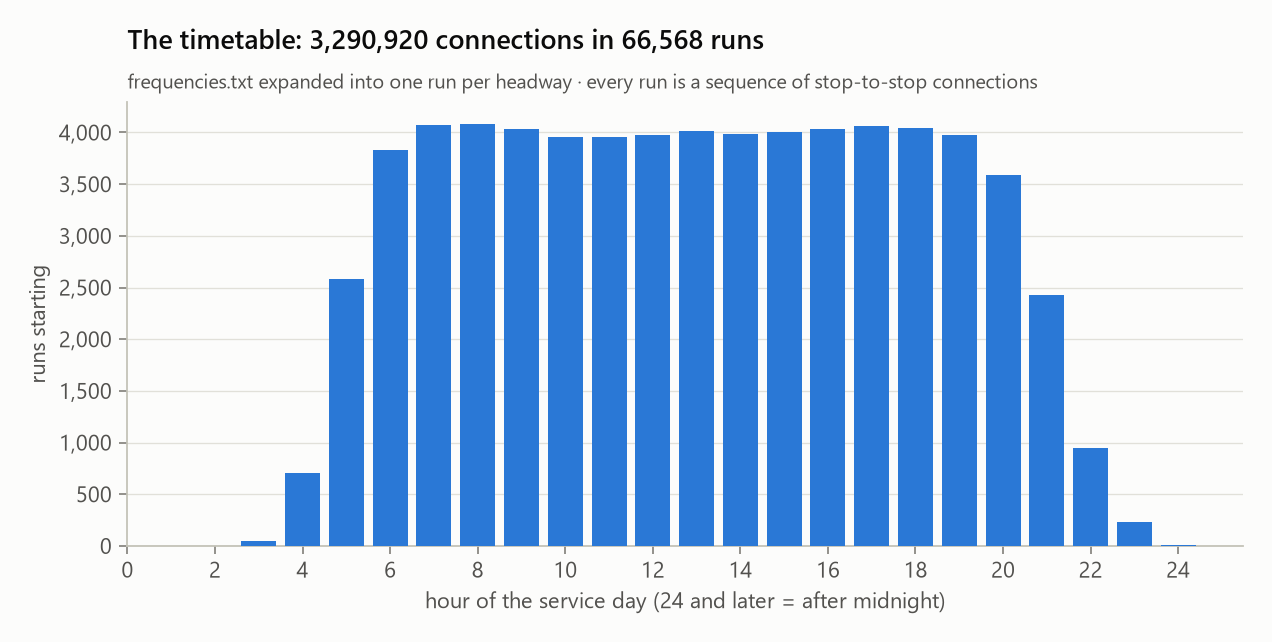
\includegraphics[width=\linewidth]{r13_timetable_by_hour.png}
    \column{0.42\textwidth}
    \scriptsize
    \textbf{\code{connections.csv.gz}} (gzip, 61\,MB) --- one row per vehicle hop, sorted by \code{dep_s}:
    \code{trip_id} (runs: \code{@HH:MM:SS}), \code{route_uid}, \code{direction_id}, \code{from_stop},
    \code{to_stop}, \code{dep_s}, \code{arr_s}, \code{time_quality}
    \vskip0.2cm
    \textbf{\code{footpaths.csv}} --- \code{self} change time (120\,s) at 10,499 stops, 226 \code{same_station},
    101,018 \code{walk} (both ways); one hop, not transitively closed
    \vskip0.2cm
    \begin{block}{Why it is large}
      66,568 runs $\times$ $\approx$49 stops = 3,290,920 connections: most mdb routes are
      ``every N minutes'' templates, expanded into real departures.
    \end{block}
    \muted{Every arc matches its connections; a CSA scan from 08:00 reaches 99.8--99.9\,\% of stops.}
  \end{columns}
\end{frame}

% ============================================================================
\begin{frame}{\step{cPTwo}{17}Export and persist}
  \vskip0.2cm
  \centering
  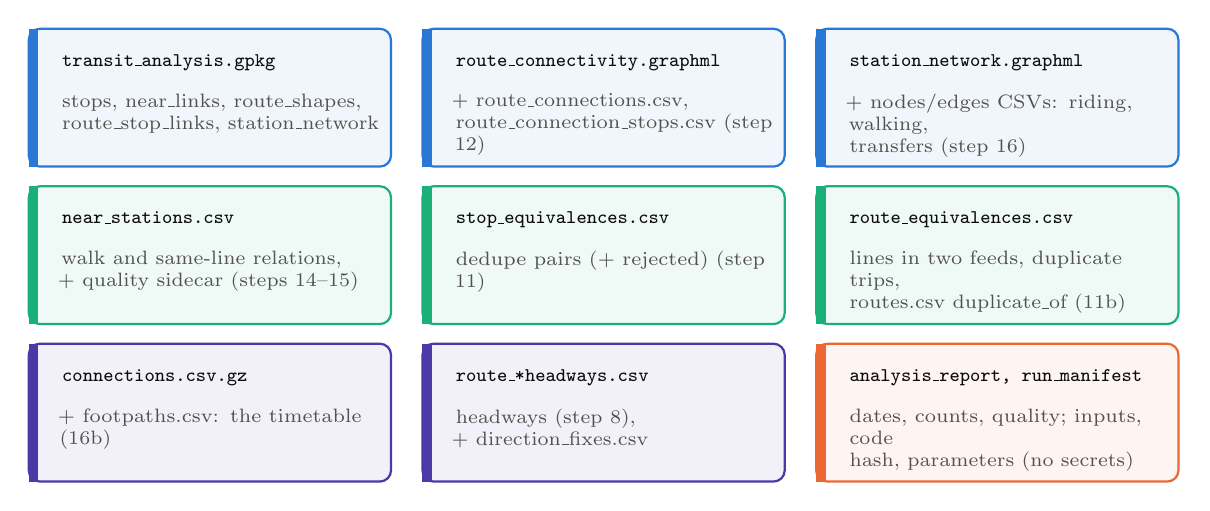
\begin{tikzpicture}[x=1cm,y=1cm]
    \foreach \x/\y/\col/\name/\what in {
      0/0/cBlue/transit\_analysis.gpkg/{stops, near\_links, route\_shapes,\\route\_stop\_links, station\_network},
      5/0/cBlue/route\_connectivity.graphml/{+ route\_connections.csv,\\route\_connection\_stops.csv (step 12)},
      10/0/cBlue/station\_network.graphml/{+ nodes/edges CSVs: riding, walking,\\transfers (step 16)},
      0/-2.0/cAqua/near\_stations.csv/{walk and same-line relations,\\+ quality sidecar (steps 14--15)},
      5/-2.0/cAqua/stop\_equivalences.csv/{dedupe pairs (+ rejected) (step 11)},
      10/-2.0/cAqua/route\_equivalences.csv/{lines in two feeds, duplicate trips,\\routes.csv duplicate\_of (11b)},
      0/-4.0/cViolet/connections.csv.gz/{+ footpaths.csv: the timetable (16b)},
      5/-4.0/cViolet/route\_*headways.csv/{headways (step 8),\\+ direction\_fixes.csv},
      10/-4.0/cOrange/{analysis\_report, run\_manifest}/{dates, counts, quality; inputs, code\\hash, parameters (no secrets)}}
    {
      \node[draw=\col, fill=\col!7, line width=0.8pt, rounded corners=4pt, minimum width=4.6cm,
            minimum height=1.75cm] at (\x+2.3,\y-0.875) {};
      \fill[\col] (\x,\y) rectangle ++(0.12,-1.75);
      \node[anchor=north west, font=\scriptsize\bfseries\ttfamily, text=cInk] at (\x+0.3,\y-0.2) {\name};
      \node[anchor=north west, font=\scriptsize, text=cInkTwo, align=left, text width=4.1cm] at (\x+0.3,\y-0.7) {\what};
    }
  \end{tikzpicture}
  \vskip0.25cm
  \muted{\scriptsize Close any QGIS layer from the GeoPackage before re-running: Windows locks the open file and the export fails.}
\end{frame}

% ============================================================================
\section{Toy model}
\divider{The network on a toy model}{cAqua}{Three sources, five routes, 13 stops --- what each step does to the graph}{%
  The model \,$\cdot$\, which steps touch the graph \,$\cdot$\, the assembled station network \,$\cdot$\, summary}

% ============================================================================
\begin{frame}{The toy model}
  \framesubtitle{Three sources, five routes, 13 stops \,$\cdot$\, analysed day: a Wednesday}
  \begin{columns}[c]
    \column{0.5\textwidth}
    \scriptsize
    \renewcommand{\arraystretch}{1.25}
    \begin{tabularx}{\linewidth}{@{}l>{\raggedright\arraybackslash}X@{}}
      \hline
      \multicolumn{2}{@{}l}{\textbf{\code{rail}} --- GTFS, light rail (\code{route_type 0})} \\ \hline
      Routes & L1: A1$\to$A2$\to$A3$\to$A4 \quad L2: A5$\to$A6 \\
      Station & A4 and A5 share \code{parent_station} ``Centro'' \\ \hline
      \multicolumn{2}{@{}l}{\textbf{\code{bus}} --- GTFS, bus (\code{route_type 3})} \\ \hline
      Routes & R10: B1$\to$B2$\to$B3 (explicit trips)\\
             & R20: B3$\to$B4$\to$B5 (\code{frequencies.txt}, every 10 min)\\
             & R30: B3$\to$B4 (Saturdays only) \\
      Names & A2 = ``Juárez'', B2 = ``JUAREZ'', 0\,m apart \\ \hline
      \multicolumn{2}{@{}l}{\textbf{\code{docks}} --- CSV \code{id, name, latitude, longitude}} \\ \hline
      Stops & M1, M2 (no routes) \\ \hline
    \end{tabularx}
    \column{0.48\textwidth}
    \centering
    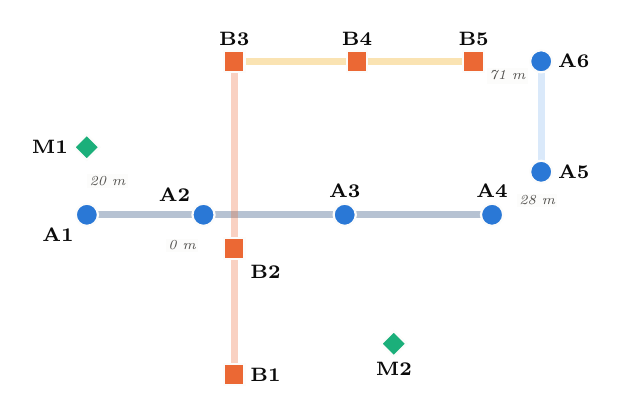
\begin{tikzpicture}[x=0.0078cm, y=0.0078cm]
      \toyCoords
      \toyLines
      \toyStops
      \toyDistances
    \end{tikzpicture}
    \vskip0.1cm
    \toyStopLegend\quad\toyRouteLegend
  \end{columns}
\end{frame}

% ============================================================================
\begin{frame}{The toy station network}
  \framesubtitle{Everything assembled into one directed graph}
  \begin{columns}[c]
    \column{0.58\textwidth}
    \centering
    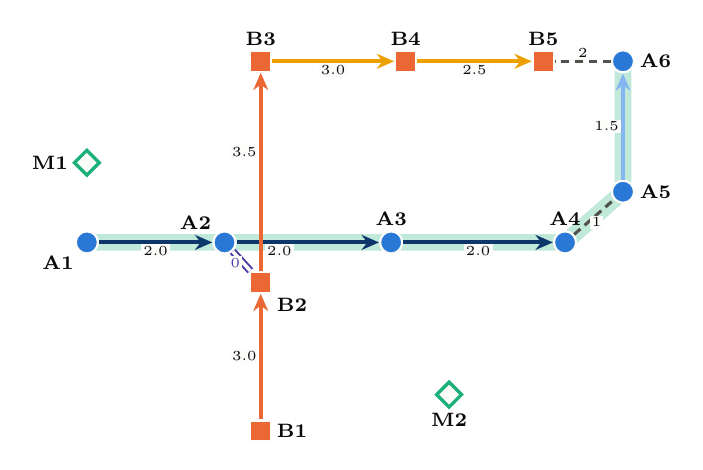
\begin{tikzpicture}[x=0.0092cm, y=0.0092cm]
      \toyCoords
      \begin{scope}[on background layer]
        \draw[pathhl] (A1) -- (A4) -- (A5) -- (A6);
      \end{scope}
      \toyStops
      \node[stBike, unlinked=cAqua] at (M1) {};
      \node[stBike, unlinked=cAqua] at (M2) {};
      \toyRides
      \draw[walkarc] (nA4) -- node[tmin, right, pos=0.35] {1} (nA5);
      \draw[walkarc] (nA6) -- node[tmin, above] {2} (nB5);
      \draw[samest] (nA2) -- node[tmin, left, pos=0.6, text=cViolet] {0} (nB2);
    \end{tikzpicture}
    \vskip0.05cm
    \toyArcLegend
    \column{0.4\textwidth}
    \scriptsize
    \renewcommand{\arraystretch}{1.25}
    \begin{tabular}{@{}l r l@{}}
      \hline
      \textbf{Element} & \textbf{Count} & \textbf{From step} \\ \hline
      nodes (stops) & 13 & 1--5 \\
      \code{in_vehicle} arcs & 8 & 6, 9 \\
      \code{walk} arcs (2 pairs) & 4 & 10, 11, 13 \\
      \code{same_station} (1 pair) & 2 & 11 \\
      unlinked dock nodes & 2 & --- \\ \hline
    \end{tabular}
    \vskip0.25cm
    \begin{exampleblock}{Shortest path A1 $\to$ A6}
      \scriptsize A1 $\xrightarrow{2+2+2}$ A4 $\xrightarrow{1}$ A5 $\xrightarrow{1.5}$ A6 \;=\; \textbf{8.5 min}\\[2pt]
      via R10/R20: $2+0+3.5+3+2.5+2 = 13$ min
    \end{exampleblock}
    \vskip0.05cm
    \muted{\tiny R30 runs on Saturdays only. A2 $\equiv$ B2 by dedupe. The docks get no arcs: walking
    through a dock would chain two 300\,m walks.}
  \end{columns}
\end{frame}

% ============================================================================
\begin{frame}{What each step does to the graph}
  \framesubtitle{Toy model: 13 nodes, 14 arcs in \code{station_network}; the timetable lists every run}
  \scriptsize
  \renewcommand{\arraystretch}{1.08}
  \begin{tabularx}{\textwidth}{@{}l c c c c c >{\raggedright\arraybackslash}X@{}}
    \hline
    \textbf{Step} & \textbf{Nodes} & \textbf{in\_vehicle} & \textbf{walk} & \textbf{same\_station} & \textbf{timetable} & \textbf{Effect in the model} \\ \hline
    1--5 ingest & \cmark & & & & & 13 stops, 2 docks unlinked later \\
    6 service date & & \cmark & & & \cmark & R30 disappears (Saturday only) \\
    7 frequencies & & & & & \cmark & R20 becomes one run every 10 min \\
    8 headways, directions & & & & & & tables only (labels fixed if mixed) \\
    9 route--stop links & & \cmark & & & \cmark & 8 timed arcs, one stop per sequence \\
    10 proximity & & & \cmark & & \cmark & candidate walk pairs \\
    11 dedupe & & & \cmark & \cmark & \cmark & A2 $\equiv$ B2: walk pair becomes same\_station \\
    11b one source per line & & \cmark & & & \cmark & (a twin line in another feed would drop) \\
    13 OSM walk & & & \cmark & & \cmark & A6--B5: 1 $\to$ 2 min \\
    16 station network & \cmark & \cmark & \cmark & \cmark & & assembles the graph \\
    16b timetable & & & & & \cmark & runs as connections + footpaths \\ \hline
    18--22 Phase 3 & & & & & & interchanges, OSM checks --- never change the graph \\ \hline
  \end{tabularx}
\end{frame}

% ============================================================================
\section{Phase 3 --- Conflation}
\divider{Phase 3 \,$\cdot$\, Conflation}{cPThree}{\code{detect-interchanges} and \code{conflate-osm}}{%
  \textbf{18} Detect interchanges \quad \textbf{19} Cross-check transfers.txt\\[5pt]
  \textbf{20} Match stops to OSM transit nodes \quad \textbf{21} Side of street \quad \textbf{22} OSM coverage gaps}

% ============================================================================
\begin{frame}[fragile]{\step{cPThree}{18}Detect interchanges}
  \framesubtitle{An interchange is infrastructure, not a schedule --- whole feed, no service date}
  \begin{columns}[T]
    \column{0.55\textwidth}
    \centering
    \resizebox{\linewidth}{!}{%
    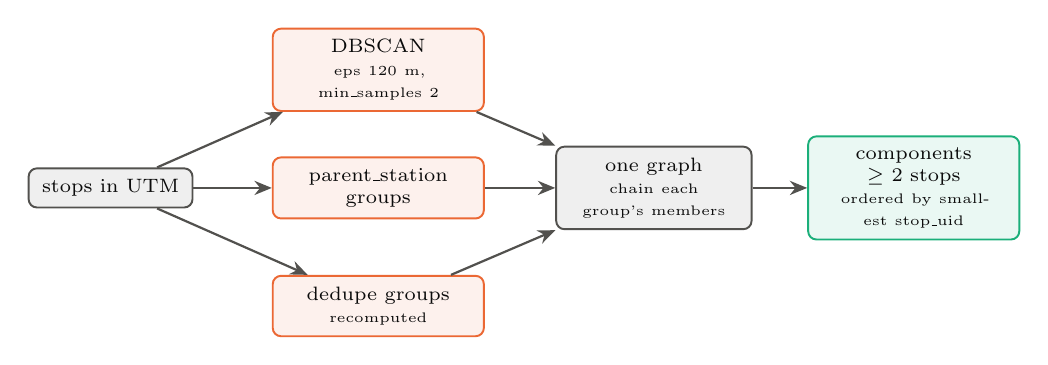
\begin{tikzpicture}[x=1cm,y=1cm]
      \node[box, text width=1.8cm] (s) at (0,0) {stops in UTM};
      \node[box=cPThree, text width=2.4cm] (db) at (3.4,1.5) {DBSCAN\\ \tiny eps 120 m, min\_samples 2};
      \node[box=cPThree, text width=2.4cm] (ps) at (3.4,0) {parent\_station groups};
      \node[box=cPThree, text width=2.4cm] (dg) at (3.4,-1.5) {dedupe groups\\ \tiny recomputed};
      \node[box, text width=2.2cm] (g) at (6.9,0) {one graph\\ \tiny chain each group's members};
      \node[box=cAqua, text width=2.4cm] (cc) at (10.2,0) {components $\ge$ 2 stops\\ \tiny ordered by smallest stop\_uid};
      \draw[arr] (s) -- (db); \draw[arr] (s) -- (ps); \draw[arr] (s) -- (dg);
      \draw[arr] (db) -- (g); \draw[arr] (ps) -- (g); \draw[arr] (dg) -- (g);
      \draw[arr] (g) -- (cc);
    \end{tikzpicture}}
\begin{lstlisting}[style=algo]
per cluster:
    modes               = distinct normalized route_type
    is_multimodal       = len(modes) > 1
    physical_stop_count = distinct canonical stations
    centroid, convex hull (EPSG:4326)
\end{lstlisting}
    \column{0.42\textwidth}
    \small
    \begin{itemize}
      \item A declared or aliased station is \textbf{never split}, even when its platforms are further apart than \code{eps}
      \item \code{route_type} normalized first: 700s $\rightarrow$ bus, 100s $\rightarrow$ rail, 400s $\rightarrow$ metro, 900s $\rightarrow$ tram
      \item \code{physical_stop_count = 1} flags a \textbf{phantom}: records of one station, not an interchange
    \end{itemize}
    \vskip0.2cm
    \begin{block}{Phase 2 vs Phase 3 dedupe}
      \scriptsize Phase 3 recomputes dedupe over the whole feed (no service date), so its route evidence and
      counts can differ from Phase 2's. Expected, not a bug.
    \end{block}
  \end{columns}
\end{frame}

% ============================================================================
\begin{frame}{\step{cPThree}{18}Interchange clusters by mode}
  \begin{columns}[c]
    \column{0.64\textwidth}
    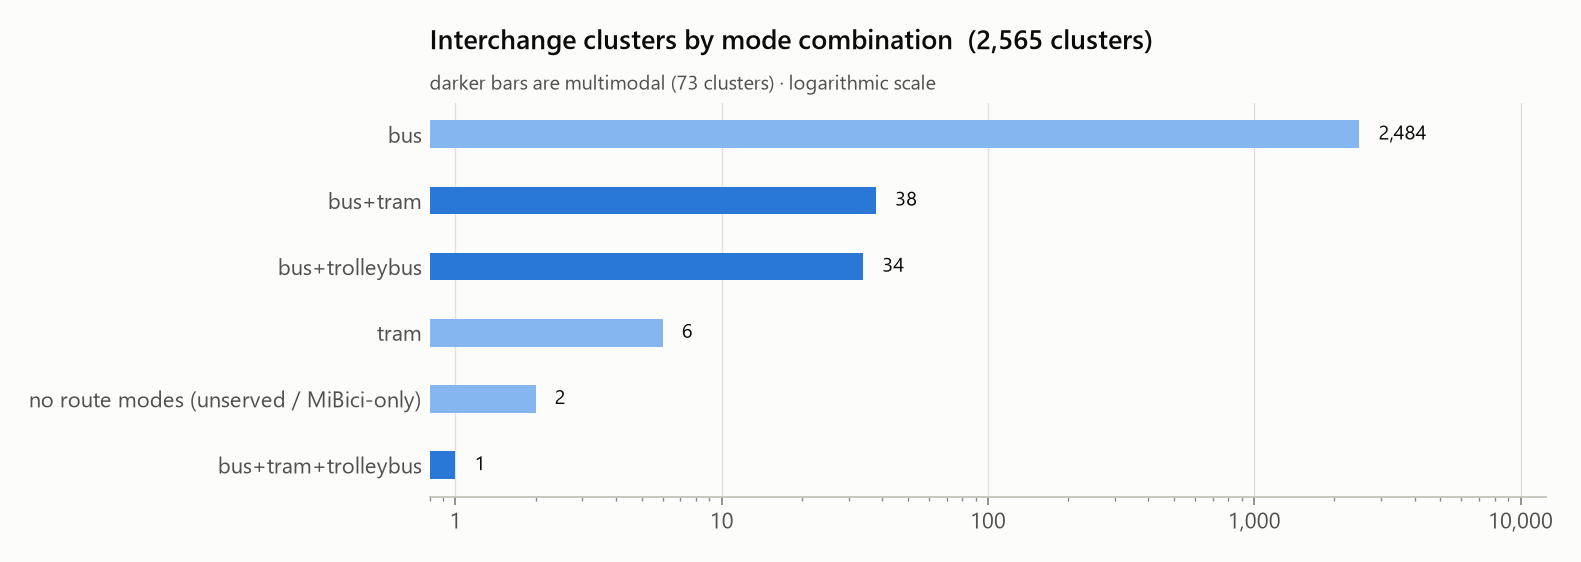
\includegraphics[width=\linewidth]{r9_interchange_modes.png}
    \column{0.34\textwidth}
    \centering
    \stat{2,565}{clusters}{cOrange}
    \vskip0.25cm
    \stat{73}{multimodal}{cBlue}
    \vskip0.25cm
    \stat{150}{single-station clusters}{cContext}
  \end{columns}
\end{frame}

% ============================================================================
\begin{frame}{\step{cPThree}{19}Cross-check transfers.txt}
  \framesubtitle{Do the clusters we inferred agree with the transfers the operator declared?}
  \vskip0.2cm
  \centering
  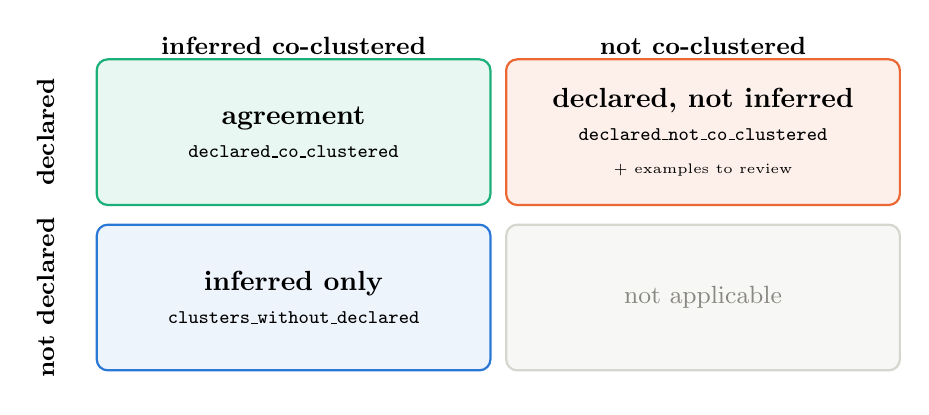
\begin{tikzpicture}[x=1cm,y=1cm]
    \node[font=\small\bfseries] at (2.6,2.5) {inferred co-clustered};
    \node[font=\small\bfseries] at (7.8,2.5) {not co-clustered};
    \node[font=\small\bfseries, rotate=90] at (-0.55,1.4) {declared};
    \node[font=\small\bfseries, rotate=90] at (-0.55,-0.7) {not declared};
    \node[draw=cAqua, fill=cAqua!10, line width=0.8pt, rounded corners=4pt, minimum width=5cm, minimum height=1.85cm, align=center]
      at (2.6,1.4) {\textbf{agreement}\\ \scriptsize\ttfamily declared\_co\_clustered};
    \node[draw=cOrange, fill=cOrange!10, line width=0.8pt, rounded corners=4pt, minimum width=5cm, minimum height=1.85cm, align=center]
      at (7.8,1.4) {\textbf{declared, not inferred}\\ \scriptsize\ttfamily declared\_not\_co\_clustered\\ \tiny + examples to review};
    \node[draw=cBlue, fill=cBlue!8, line width=0.8pt, rounded corners=4pt, minimum width=5cm, minimum height=1.85cm, align=center]
      at (2.6,-0.7) {\textbf{inferred only}\\ \scriptsize\ttfamily clusters\_without\_declared};
    \node[draw=cContext, fill=cContext!20, line width=0.8pt, rounded corners=4pt, minimum width=5cm, minimum height=1.85cm, align=center, text=cMuted]
      at (7.8,-0.7) {\small not applicable};
  \end{tikzpicture}
  \vskip0.3cm
  \muted{\small A feed without \code{transfers.txt} is listed in \code{feeds_without_transfers} --- not an error.}
\end{frame}

% ============================================================================
\begin{frame}[fragile]{\step{cPThree}{20}Match stops to OSM transit nodes}
  \begin{columns}[T]
    \column{0.46\textwidth}
\begin{lstlisting}[style=sql]
SELECT s.stop_uid, o.osm_id, o.kind, o.distance_m
FROM stops s
LEFT JOIN LATERAL (
  SELECT p.osm_id, ... AS kind,
    ST_Distance(s.geom::geography,
      ST_Transform(p.way,4326)::geography)
      AS distance_m
  FROM planet_osm_point p
  WHERE p.highway = 'bus_stop'
     OR p.public_transport IN
        ('platform','stop_position','station')
     OR p.railway IN ('station','halt','tram_stop')
  ORDER BY p.way <-> ST_Transform(s.geom, srid)
  LIMIT 1                        -- index KNN
) o ON TRUE;
\end{lstlisting}
    \column{0.52\textwidth}
    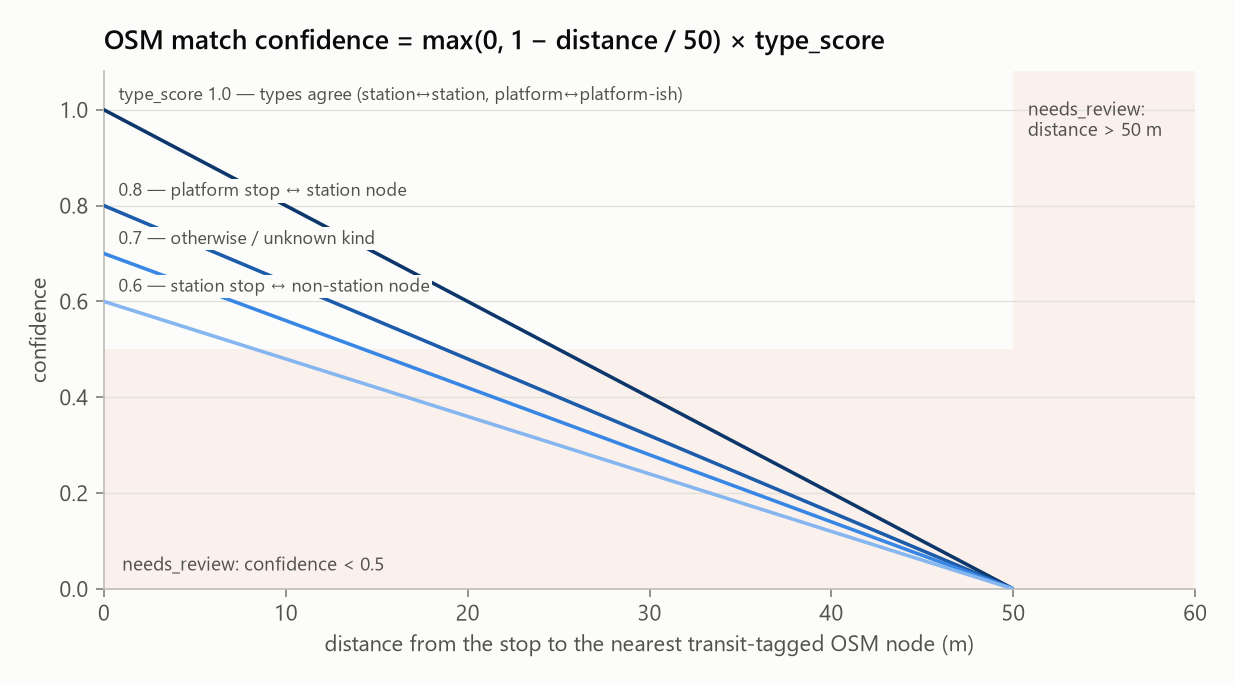
\includegraphics[width=\linewidth]{e4_osm_confidence.png}
    \vskip0.1cm
    \scriptsize
    \begin{itemize}
      \item $\mathit{confidence} = \max(0,\ 1 - d/50) \times \mathit{type\_score}$
      \item \code{needs_review} $\Leftarrow$ no candidate, $d > 50$\,m, or confidence $< 0.5$
      \item Schema validated first; fails fast listing every problem
    \end{itemize}
  \end{columns}
\end{frame}

% ============================================================================
\begin{frame}{\step{cPThree}{20}OSM confidence by source}
  \centering
  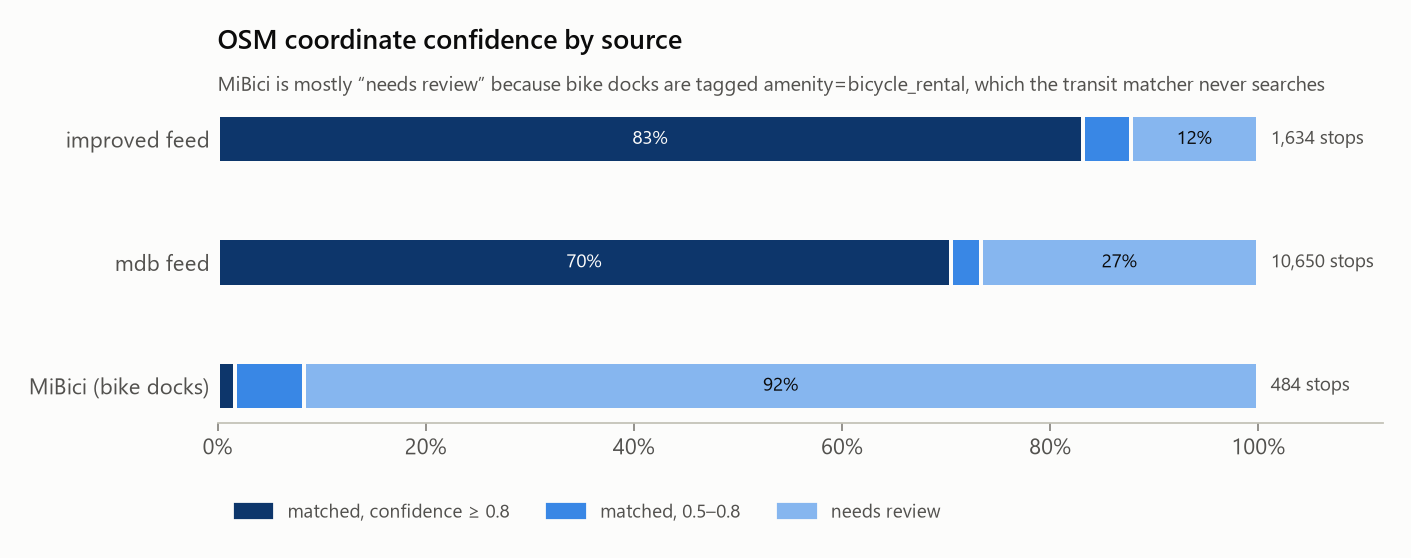
\includegraphics[width=0.78\textwidth]{r10_osm_match_outcomes.png}
  \vskip0.1cm
  \begin{columns}[T]
    \column{0.3\textwidth}\centering\stat{73.1\%}{stops matched overall}{cBlue}
    \column{0.66\textwidth}
    \begin{alertblock}{MiBici's 92\% ``needs review'' is a matcher-scope result}
      \scriptsize The query searches public-transport tags only. Bike docks are tagged
      \code{amenity=bicycle_rental} and are never searched, so a dock that sits exactly on its OSM node
      still comes back without a match. It is not evidence of bad coordinates.
    \end{alertblock}
  \end{columns}
\end{frame}

% ============================================================================
\begin{frame}{\step{cPThree}{21}Determine side of street}
  \centering
  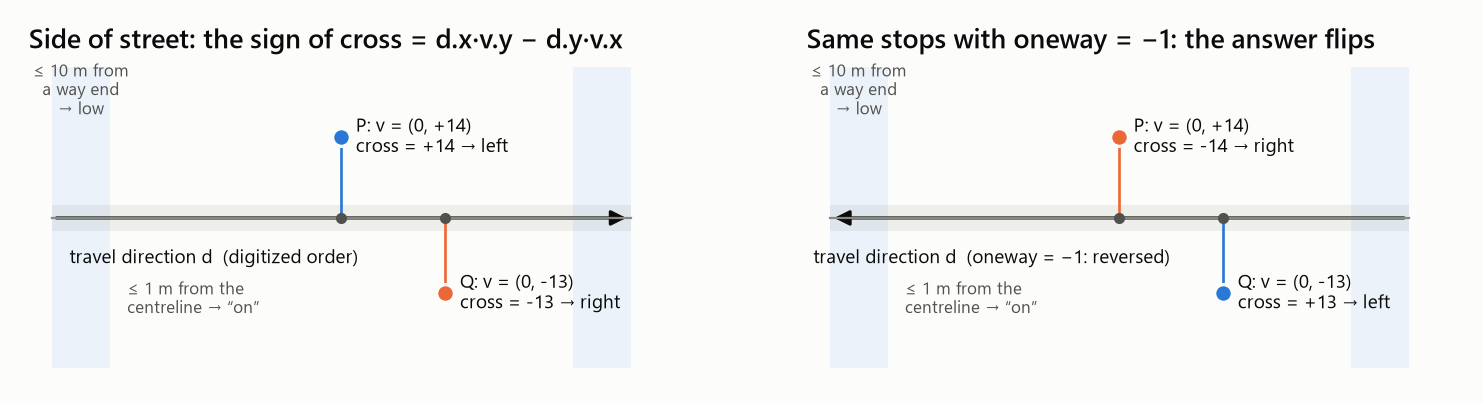
\includegraphics[width=0.92\textwidth]{e3_side_of_street.png}
  \vskip0.1cm
  \begin{columns}[T]
    \column{0.47\textwidth}
    \begin{block}{Rule}
      \scriptsize nearest highway centerline (KNN, $\le$ 50\,m) $\rightarrow$ nearest segment in UTM\\
      $d$ = direction \emph{of travel} (reversed when \code{oneway = -1})\\
      $v$ = stop minus its perpendicular foot\\
      $\mathit{cross} = d_x v_y - d_y v_x$: \ $>0$ left, \ $<0$ right, \ $|v| \le 1$\,m on
    \end{block}
    \column{0.49\textwidth}
    \begin{alertblock}{Low confidence when}
      \scriptsize side is \code{on} \,$\cdot$\, foot within 10\,m of a way end (an intersection) \,$\cdot$\,
      $|v| < 2$\,m\\[3pt]
      Two-way streets: side is relative to OSM digitization. Rail stations snap to the nearest road;
      centre-median BRT platforms land in \code{on}.
    \end{alertblock}
  \end{columns}
\end{frame}

% ============================================================================
\begin{frame}{\step{cPThree}{22}Find OSM coverage gaps}
  \framesubtitle{The reverse question: what transit does OSM know that the feeds don't?}
  \begin{columns}[c]
    \column{0.5\textwidth}
    \centering
    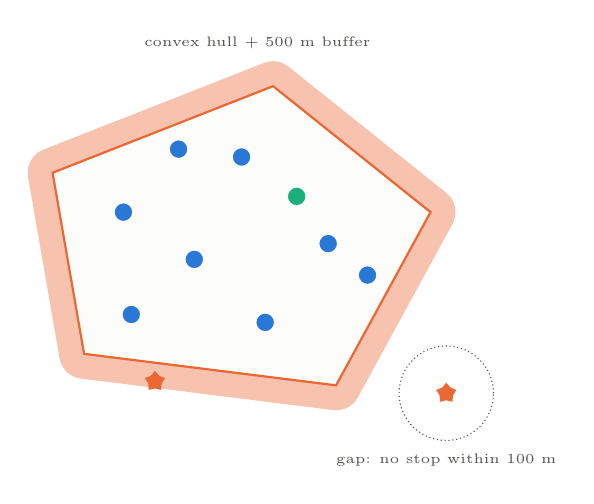
\begin{tikzpicture}[x=1cm,y=1cm]
      \coordinate (h1) at (0,0); \coordinate (h2) at (3.2,-0.4); \coordinate (h3) at (4.4,1.8);
      \coordinate (h4) at (2.4,3.4); \coordinate (h5) at (-0.4,2.3);
      \draw[cOrange!40, line width=18pt, line join=round] (h1) -- (h2) -- (h3) -- (h4) -- (h5) -- cycle;
      \fill[cSurface] (h1) -- (h2) -- (h3) -- (h4) -- (h5) -- cycle;
      \draw[cOrange, line width=0.8pt] (h1) -- (h2) -- (h3) -- (h4) -- (h5) -- cycle;
      \foreach \p in {(0.6,0.5),(1.4,1.2),(2.3,0.4),(3.1,1.4),(2.0,2.5),(0.5,1.8),(3.6,1.0),(1.2,2.6)}
        \node[stop=cBlue] at \p {};
      \node[stop=cAqua] (ok) at (2.7,2.0) {};
      \node[star, star points=5, fill=cOrange, inner sep=1.8pt] (gap) at (4.6,-0.5) {};
      \node[star, star points=5, fill=cOrange, inner sep=1.8pt] at (0.9,-0.35) {};
      \draw[cInkTwo, densely dotted] (gap) circle (0.6);
      \node[lbl, anchor=north] at (4.6,-1.15) {gap: no stop within 100 m};
      \node[lbl, anchor=south] at (2.2,3.75) {convex hull + 500 m buffer};
    \end{tikzpicture}
    \column{0.48\textwidth}
    \begin{block}{Algorithm}
      \small
      \begin{enumerate}\scriptsize
        \item $\mathit{area} = \mathrm{buffer}(\mathrm{hull}(\text{all stops}), 500\,\mathrm{m})$
        \item Each OSM transit node inside the area
        \item Nearest stop by KNN, measured geodesically
        \item Keep it if that stop is $>$ 100\,m away
        \item Sort worst gap first
      \end{enumerate}
    \end{block}
    \vskip0.2cm
    \small A \textbf{review list, not a verdict}: a gap is either a hole in the feeds or noise in OSM.
    \vskip0.2cm
    \stat{34}{OSM-only transit nodes}{cOrange}
  \end{columns}
\end{frame}

% ============================================================================
\section{Phase 4 --- External checks}
\divider{Phase 4 \,$\cdot$\, External checks}{cPFour}{Opt-in, budgeted, nothing stored but verdicts}{%
  \textbf{24} Google QA and station locator}

% ============================================================================
\begin{frame}{\step{cPFour}{24}Google QA and station locator}
  \framesubtitle{Off by default --- a flag \emph{and} an API key in the environment are both required}
  \begin{columns}[T]
    \column{0.55\textwidth}
    \centering
    \resizebox{\linewidth}{!}{%
    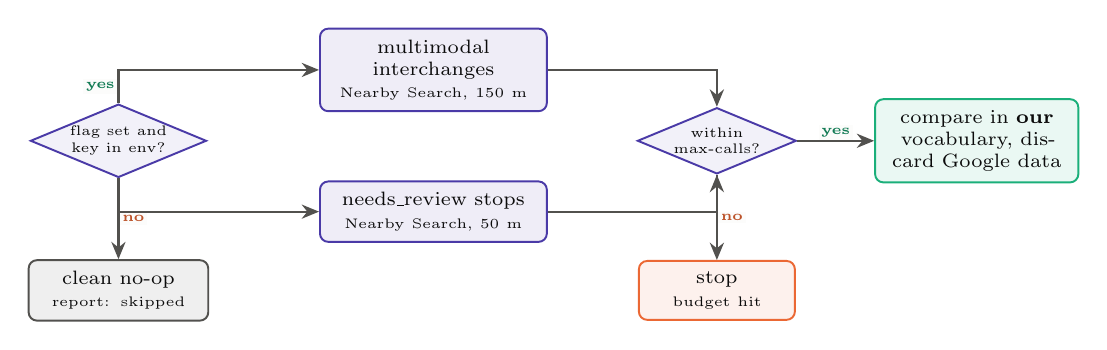
\begin{tikzpicture}[x=1cm,y=1cm]
      \node[dec=cPFour] (g) at (0,0) {flag set and\\key in env?};
      \node[box, text width=2.0cm] (noop) at (0,-1.9) {clean no-op\\ \tiny report: skipped};
      \node[box=cPFour, text width=2.6cm] (mi) at (4,0.9) {multimodal interchanges\\ \tiny Nearby Search, 150 m};
      \node[box=cPFour, text width=2.6cm] (nr) at (4,-0.9) {needs\_review stops\\ \tiny Nearby Search, 50 m};
      \node[dec=cPFour] (bud) at (7.6,0) {within\\max-calls?};
      \node[box=cOrange, text width=1.7cm] (stop) at (7.6,-1.9) {stop\\ \tiny budget hit};
      \node[box=cAqua, text width=2.3cm] (v) at (10.9,0) {compare in \textbf{our} vocabulary, discard Google data};
      \draw[arr] (g) -- node[no, right] {no} (noop);
      \draw[arr] (g) |- node[yes, pos=0.25, left] {yes} (mi);
      \draw[arr] (g) |- (nr);
      \draw[arr] (mi) -| (bud); \draw[arr] (nr) -| (bud);
      \draw[arr] (bud) -- node[no, right] {no} (stop);
      \draw[arr] (bud) -- node[yes, above] {yes} (v);
    \end{tikzpicture}}
    \column{0.43\textwidth}
    \scriptsize
    \renewcommand{\arraystretch}{1.3}
    \begin{tabularx}{\linewidth}{@{}l>{\raggedright\arraybackslash}X@{}}
      \hline
      \textbf{Target} & \textbf{Verdicts} \\ \hline
      interchanges & CONFIRMED, PARTIAL, CONFLICT, NO\_DATA \\
      stops & STATION\_FOUND, NOT\_FOUND, NO\_DATA \\ \hline
    \end{tabularx}
    \vskip0.3cm
    \begin{alertblock}{Licensing rails, enforced in code}
      \scriptsize Only the opaque \code{place_id} and the verdict are stored --- a frozen column allowlist.
      No names, coordinates or lines, in the database, files or logs.
    \end{alertblock}
    \vskip0.15cm
    \muted{The station locator resolves station names and travel times, exports Excel, never writes to the database.}
  \end{columns}
\end{frame}

% ============================================================================
\section{Results}
\divider{Results}{cInk}{The data model, the numbers, and how to read them}{%
  Data model \,$\cdot$\, Guadalajara in numbers \,$\cdot$\, choosing the proximity threshold
  \\[4pt] interpretation pitfalls \,$\cdot$\, parameters \,$\cdot$\, reproducing the run}

% ============================================================================
\begin{frame}{The data model}
  \framesubtitle{Every analysis table keys back to \code{stops} --- nothing is ever deleted from it}
  \centering
  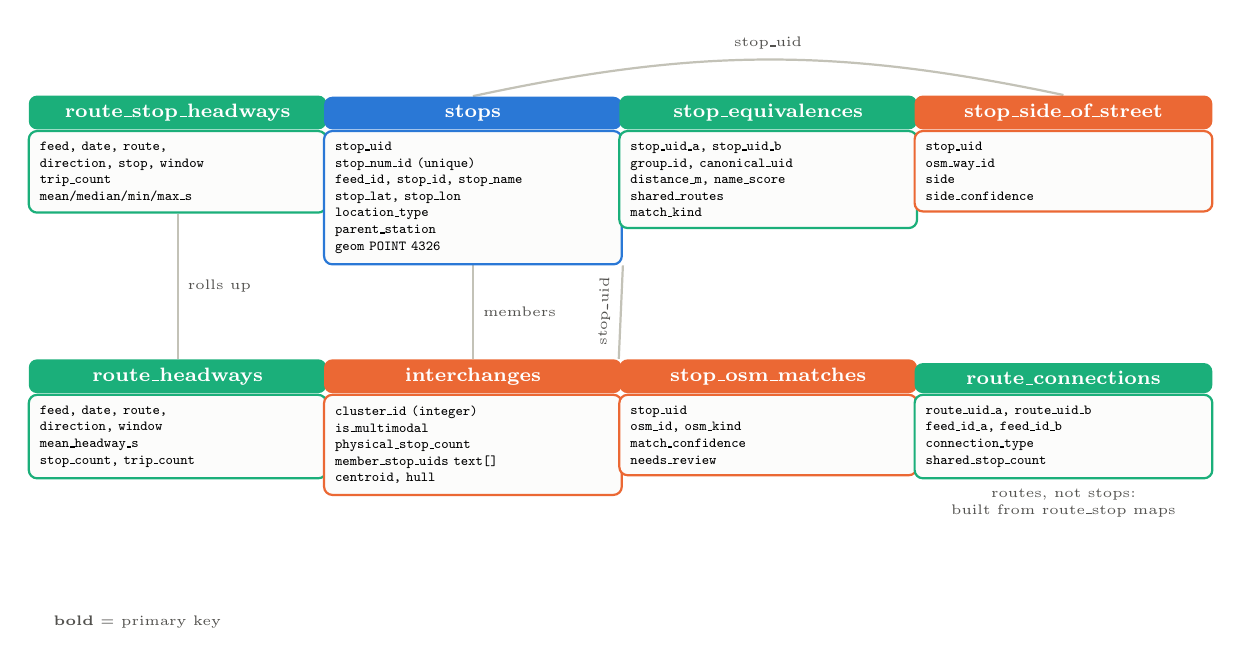
\begin{tikzpicture}[x=1cm,y=1cm, rel/.style={line width=0.8pt, cBase}]
    % top row
    \tb{rsh}{route\_stop\_headways}{cPTwo}{0}{3.0}{\textbf{feed, date, route,}\\\textbf{direction, stop, window}\\trip\_count\\mean/median/min/max\_s}
    \tb{stops}{stops}{cPOne}{3.75}{3.0}{\textbf{stop\_uid}\\stop\_num\_id (unique)\\feed\_id, stop\_id, stop\_name\\stop\_lat, stop\_lon\\location\_type\\parent\_station\\geom POINT 4326}
    \tb{eq}{stop\_equivalences}{cPTwo}{7.5}{3.0}{\textbf{stop\_uid\_a, stop\_uid\_b}\\group\_id, canonical\_uid\\distance\_m, name\_score\\shared\_routes\\match\_kind}
    \tb{ss}{stop\_side\_of\_street}{cPThree}{11.25}{3.0}{\textbf{stop\_uid}\\osm\_way\_id\\side\\side\_confidence}
    % bottom row
    \tb{rh}{route\_headways}{cPTwo}{0}{-0.35}{\textbf{feed, date, route,}\\\textbf{direction, window}\\mean\_headway\_s\\stop\_count, trip\_count}
    \tb{ic}{interchanges}{cPThree}{3.75}{-0.35}{\textbf{cluster\_id} (integer)\\is\_multimodal\\physical\_stop\_count\\member\_stop\_uids text[]\\centroid, hull}
    \tb{om}{stop\_osm\_matches}{cPThree}{7.5}{-0.35}{\textbf{stop\_uid}\\osm\_id, osm\_kind\\match\_confidence\\needs\_review}
    \tb{rc}{route\_connections}{cPTwo}{11.25}{-0.35}{\textbf{route\_uid\_a, route\_uid\_b}\\feed\_id\_a, feed\_id\_b\\connection\_type\\shared\_stop\_count}
    % relations
    \begin{scope}[on background layer]
      \draw[rel] (rsh.east |- 0,2.2) -- node[lbl, above] {feed, stop} (stops.west |- 0,2.2);
      \draw[rel] (rsh.south) -- node[lbl, right] {rolls up} (rhh.north);
      \draw[rel] (stops.south) -- node[lbl, right] {members} (ich.north);
      \draw[rel] (stops.east |- 0,2.2) -- node[lbl, above] {stop\_uid} (eq.west |- 0,2.2);
      \draw[rel] (stops.south east) -- node[lbl, sloped, above] {stop\_uid} (omh.north west);
      \draw[rel] (stopsh.north) to[bend left=12] node[lbl, above, pos=0.5] {stop\_uid} (ssh.north);
    \end{scope}
    \node[lbl, anchor=north, align=center] at (rc.south) {routes, not stops:\\built from route\_stop maps};
    \node[anchor=west, font=\tiny, text=cInkTwo] at (-1.7,-3.25) {\textbf{bold} = primary key};
  \end{tikzpicture}
\end{frame}

% ============================================================================
\begin{frame}{Guadalajara in numbers}
  \framesubtitle{Two GTFS feeds and the MiBici stops CSV \,$\cdot$\, OSM network walk \,$\cdot$\, 300\,m proximity}
  \vskip0.2cm
  \centering
  \resizebox{\textwidth}{!}{%
  \begin{tabular}{@{}cccc@{}}
    \stat{14,349}{stop records, 0 errors}{cPOne} & \stat{10,203}{physical stations}{cPTwo} &
    \stat{2,812}{dedupe pairs (772 rejected)}{cPTwo} & \stat{249 / 7,902}{routing lines / route links}{cPTwo} \\[6pt]
    \stat{107,398}{stop-level headway rows}{cPTwo} & \stat{174,232}{station-network arcs, 1 component}{cPTwo} &
    \stat{1.35$\times$}{typical walk detour}{cPTwo} & \stat{3.29\,M}{timetable connections}{cPTwo} \\[6pt]
    \stat{2,565}{interchange clusters}{cPThree} & \stat{73.1\%}{stops matched to OSM}{cPThree} &
    \stat{67\%}{stops right of street (27\% left)}{cPThree} & \stat{484}{MiBici docks, 0 merged}{cAqua} \\
  \end{tabular}}
  \vskip0.25cm
  \muted{\scriptsize Service dates: typical weekday 2021-05-04 (improved) and 2024-06-27 (mdb). The calendars never
  overlap, so cross-feed outputs combine two years; after route dedupe only 2 improved routes remain in routing.}
\end{frame}

% ============================================================================
\begin{frame}{Choosing the proximity threshold}
  \begin{columns}[c]
    \column{0.63\textwidth}
    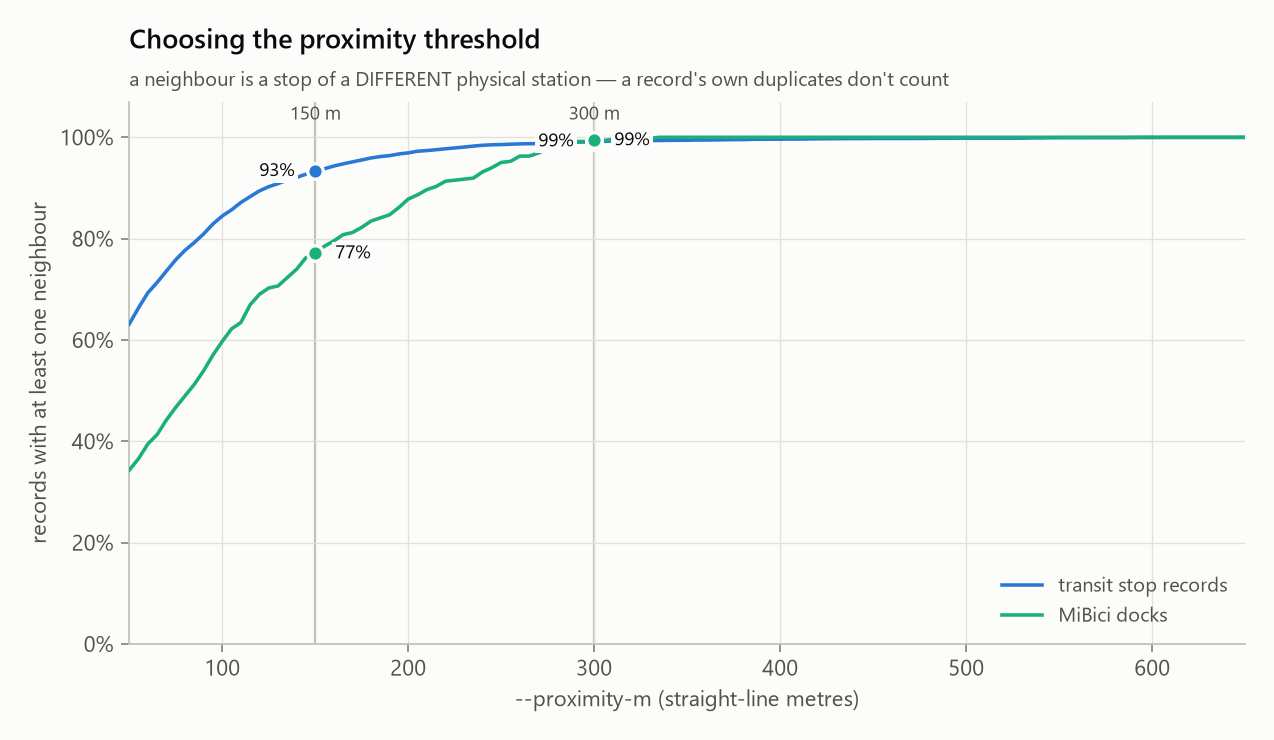
\includegraphics[width=\linewidth]{r6_proximity_threshold.png}
    \column{0.35\textwidth}
    \small
    A neighbour is a stop of a \textbf{different} physical station --- a record's own duplicates don't count.
    \vskip0.3cm
    \scriptsize
    \renewcommand{\arraystretch}{1.35}
    \begin{tabularx}{\linewidth}{@{}>{\raggedright\arraybackslash}X r r@{}}
      \hline
      & \textbf{150\,m} & \textbf{300\,m} \\ \hline
      transit records with a neighbour & 93\% & 99\% \\
      MiBici docks with a neighbour & 77\% & 99\% \\
      isolated records & 934 & 106 \\ \hline
    \end{tabularx}
    \vskip0.25cm
    \muted{300\,m $\approx$ a 3--4 minute walk.}
  \end{columns}
\end{frame}

% ============================================================================
\begin{frame}{Where the isolated stop records are}
  \begin{columns}[c]
    \column{0.47\textwidth}
    \centering
    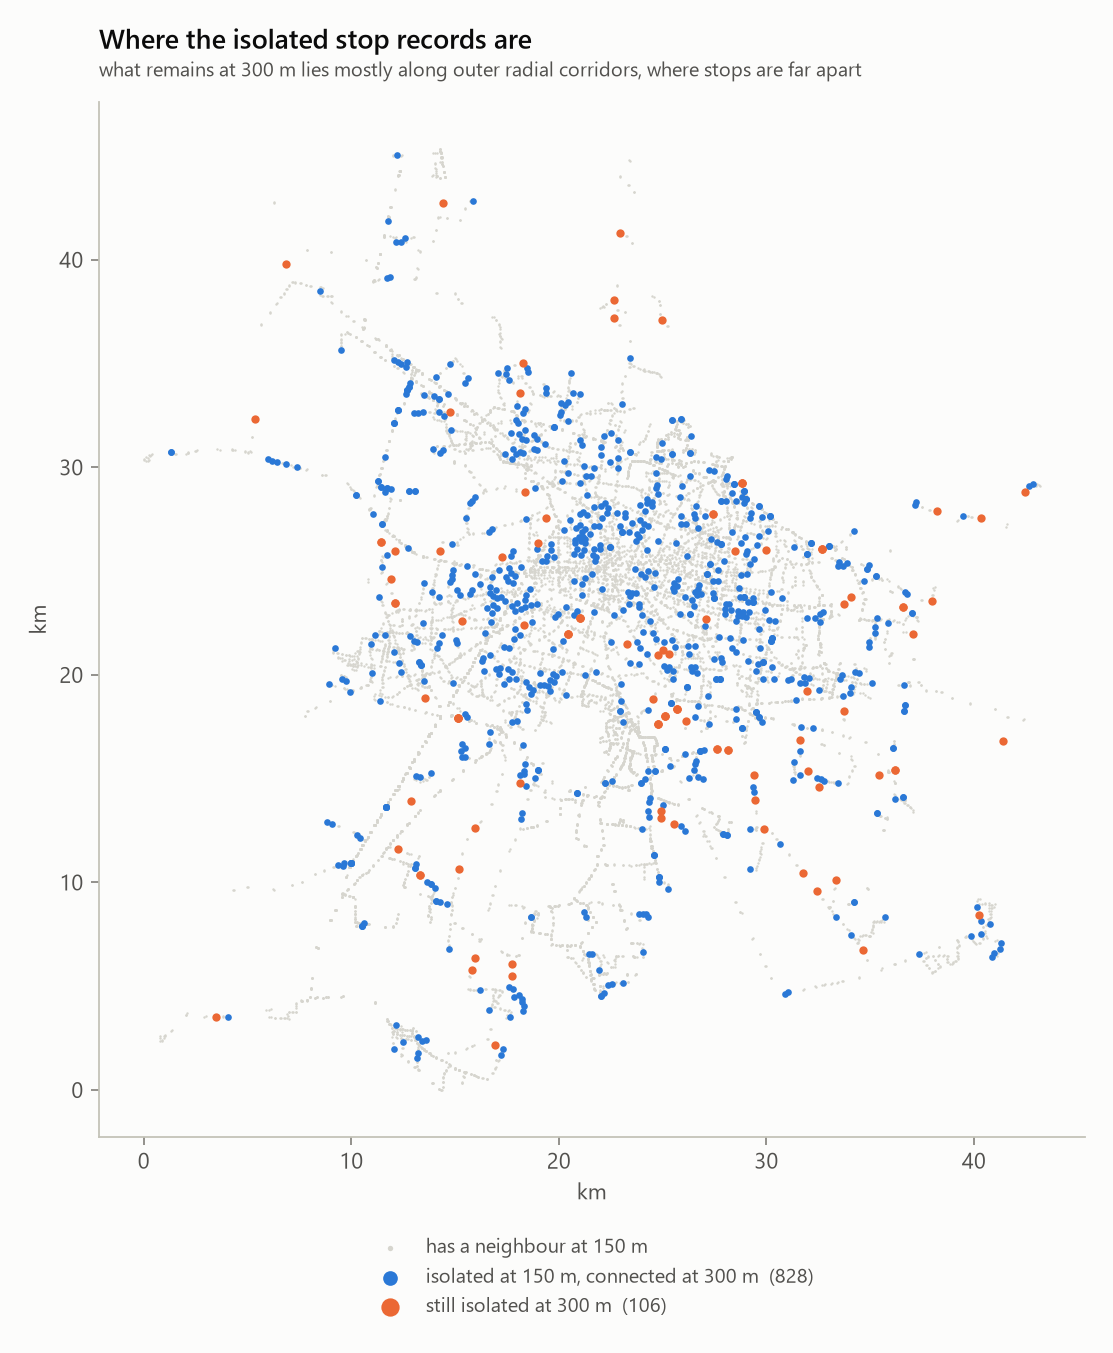
\includegraphics[height=0.86\textheight]{r7_isolation_map.png}
    \column{0.51\textwidth}
    \small
    \begin{itemize}
      \item \textcolor{cBlue}{\textbf{828}} records were isolated at 150\,m and connect at 300\,m ---
            mostly inside the urban area
      \item \textcolor{cOrange!85!black}{\textbf{106}} remain isolated --- mostly along outer radial corridors,
            where consecutive stops really are far apart
    \end{itemize}
    \vskip0.3cm
    \begin{alertblock}{A threshold changes more than neighbour lists}
      \scriptsize \code{--proximity-m} also creates route \code{proximity} edges and station-network walk arcs.
      Compare connectivity figures only between runs with the same threshold.
    \end{alertblock}
  \end{columns}
\end{frame}

% ============================================================================
\begin{frame}{Interpretation pitfalls}
  \begin{columns}[T]
    \column{0.49\textwidth}
    \small
    \begin{enumerate}
      \setlength{\itemsep}{3pt}
      \item \textbf{Records are not stations.} Count with \code{COALESCE(station_dedup, stop_uid)}.
      \item \textbf{A station is a platform group}: opposite platforms are separate stations, joined by walking.
      \item \textbf{Check} \code{service_dates_coherent}: here the feeds' calendars never overlap.
      \item \textbf{\code{direction_id} is unreliable} in the source; the pipeline relabels mixed routes.
      \item \textbf{Count routes in routing} with \code{duplicate_of} empty: 249, not 287.
      \item \textbf{Headways don't vary by time of day} because the source data doesn't.
    \end{enumerate}
    \column{0.49\textwidth}
    \small
    \begin{enumerate}\setcounter{enumi}{6}
      \setlength{\itemsep}{3pt}
      \item \textbf{Use the median detour} (1.35$\times$), not the mean.
      \item \textbf{\code{needs_review} for bike docks} is matcher scope, not bad coordinates.
      \item \textbf{\code{-} in a near-stations tuple} marks a neighbour no line serves.
      \item \textbf{Filter on \code{time_quality}} before trusting an in-vehicle time.
      \item \textbf{Footpaths are one hop}: CSA needs them closed, or an algorithm that walks twice.
    \end{enumerate}
  \end{columns}
\end{frame}

% ============================================================================
\begin{frame}{Parameters that shape the results}
  \scriptsize
  \renewcommand{\arraystretch}{1.12}
  \vskip0.2cm
  \centering
  \resizebox{\textwidth}{!}{%
  \begin{tabular}{@{}l r r l @{\hspace{2.2em}} l r r l@{}}
    \hline
    \textbf{Parameter} & \textbf{Default} & \textbf{Step} & \textbf{Controls} &
    \textbf{Parameter} & \textbf{Default} & \textbf{Step} & \textbf{Controls} \\ \hline
    \code{--service-date} / \code{--date-rule} & typical weekday & 6 & day analysed & \code{--route-dedupe} & on & 11b & one source per line \\
    \code{--feed-service-date} & --- & 6 & pin one feed & \code{--network-walk} & off & 13 & OSM streets \\
    \code{--common-date} & off & 6 & one shared day & \code{--prune-station-network} & off & 16 & redundant arcs \\
    \code{--window} & 4 & 8 & headway windows & \code{--min-transfer-s} & 120 & 16b & change time \\
    \code{--fix-directions} & on & 8 & relabel mixed routes & \code{--eps} & 120 & 18 & DBSCAN radius \\
    \code{--transport-mode}, \code{--route} & all & 6--9 & routes kept & \code{--min-samples} & 2 & 18 & DBSCAN core \\
    \code{--drop-unserved-stops} & on & 4 & never-served stops & \code{--match-threshold-m} & 50 & 20 & OSM match \\
    \code{--proximity-m} & 150 & 10--16 & ``near'' & \code{--street-threshold-m} & 50 & 21 & centerline \\
    \code{--dedupe-distance-m} & 30 & 11 & cross-feed radius & \code{--coverage-radius-m} & 100 & 22 & gap radius \\
    \code{--dedupe-name-threshold} & 0.75 & 11 & name similarity & \code{--coverage-buffer-m} & 500 & 22 & service area \\
    \code{--dedupe-within-feed-distance-m} & 5 & 11 & within-feed radius & \code{--max-calls} & 200 & 24 & Google budget \\ \hline
  \end{tabular}}
  \raggedright
  \vskip0.5cm
  \begin{block}{Fixed constants}
    \small walking 83\,m/min \,$\cdot$\, vehicle fallback 25\,km/h \,$\cdot$\, vertex grid 0.1\,m
    \,$\cdot$\, Dijkstra limit 800\,m \,$\cdot$\, snap label 200\,m \,$\cdot$\, at most 1,000 runs per frequency row
    \,$\cdot$\, route match Jaccard 0.8 \,$\cdot$\, \code{too_fast} 80\,km/h, \code{too_slow} 5\,km/h
  \end{block}
\end{frame}

% ============================================================================
\begin{frame}[fragile]{Reproduce this run}
  \begin{columns}[T]
    \column{0.6\textwidth}
\begin{lstlisting}[style=algo]
FEEDS="improved-gtfs-mimacro-mitren-sitren.zip
       mdb-2366-202502241922.zip mibici.csv"

OUT=outputs/out_mibici_v12
python -m gtfs_ingest.cli ingest --feeds $FEEDS \
    --report $OUT --analysis-date 2026-10-31
python -m gtfs_ingest.cli analyze-frequency \
    --feeds $FEEDS --report $OUT \
    --network-walk --proximity-m 300
python -m gtfs_ingest.cli detect-interchanges \
    --feeds $FEEDS --report $OUT
python -m gtfs_ingest.cli conflate-osm --report $OUT
python -m gtfs_ingest.cli analyze-frequency ...   # pass 2

python docs/figures/make_figures.py --run $OUT
\end{lstlisting}
    \column{0.37\textwidth}
    \begin{block}{Go deeper (\code{docs/guide/})}
      \scriptsize
      \begin{itemize}
        \item \code{pipeline-guide.md}: every step and pitfall
        \item \code{workflow.md}: the data, by concern
        \item \code{data-dictionary.md}: every column
        \item \code{README.md}: install and operate
      \end{itemize}
    \end{block}
    \vskip0.2cm
    \muted{\tiny Two runs give byte-identical files; \code{run_manifest.json} records inputs, code hash and
    parameters. \code{--dry-run} skips the database.}
  \end{columns}
\end{frame}

% ============================================================================
\begin{frame}{What the outputs enable: routing}
  \framesubtitle{Two inputs, two families of algorithms}
  \begin{columns}[T]
    \column{0.48\textwidth}
    \begin{block}{\code{station_network.graphml} --- a static graph}
      \scriptsize Nodes = stops, arcs weighted by minutes (scheduled ride, walk, 0-min alias).\\[3pt]
      \textbf{Dijkstra} gives travel time \emph{without waiting}: a lower bound, useful as a baseline.
      Frequencies could add an expected wait per boarding.
    \end{block}
    \column{0.48\textwidth}
    \begin{block}{\code{connections.csv.gz} + \code{footpaths.csv} --- a timetable}
      \scriptsize Every departure of the day, plus change and walk times.\\[3pt]
      \textbf{CSA}, \textbf{RAPTOR} and \textbf{time-dependent Dijkstra} give earliest arrival from a
      departure time, with waiting and transfers.
    \end{block}
  \end{columns}
  \vskip0.3cm
  \begin{columns}[T]
    \column{0.48\textwidth}
    \begin{exampleblock}{Already in place}
      \scriptsize one source per line \,$\cdot$\, a typical weekday \,$\cdot$\, directions fixed \,$\cdot$\,
      time quality labels \,$\cdot$\, deterministic outputs
    \end{exampleblock}
    \column{0.48\textwidth}
    \begin{alertblock}{Next}
      \scriptsize frequency-based graph (waiting cost) \,$\cdot$\, access and egress from any point \,$\cdot$\,
      a common algorithm interface \,$\cdot$\, query sets and metrics \,$\cdot$\, comparison with OpenTripPlanner / r5py
    \end{alertblock}
  \end{columns}
\end{frame}

% ============================================================================
\section{Glossary}
\begin{frame}{Glossary: graphs and connectivity}
  \begin{columns}[T]
    \column{0.5\textwidth}
    \centering
    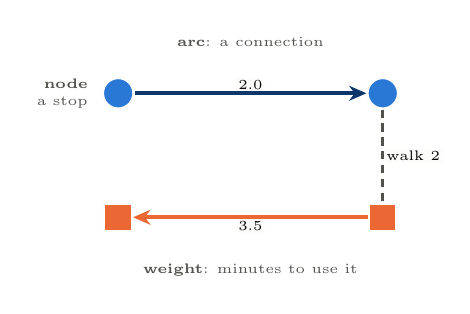
\begin{tikzpicture}[x=1.05cm, y=1.05cm]
      \node[stRail, minimum size=11pt] (p) at (0,1.5) {};
      \node[stRail, minimum size=11pt] (q) at (3.2,1.5) {};
      \node[stBus, minimum size=10pt] (r) at (3.2,0) {};
      \node[stBus, minimum size=10pt] (t) at (0,0) {};
      \draw[ride=cLone] (p) -- node[tmin, above] {2.0} (q);
      \draw[walkarc] (q) -- node[tmin, right] {walk 2} (r);
      \draw[ride=cRten] (r) -- node[tmin, below] {3.5} (t);
      \node[lbl, anchor=east, align=right] at (-0.25,1.5) {\textbf{node}\\a stop};
      \node[lbl, anchor=south, align=center] at (1.6,1.95) {\textbf{arc}: a connection};
      \node[lbl, anchor=north, align=center] at (1.6,-0.45) {\textbf{weight}: minutes to use it};
    \end{tikzpicture}
    \vskip0.3cm
    \scriptsize
    \begin{itemize}
      \item A \textbf{graph} is a set of nodes joined by arcs; a ride runs one way, a walk both ways.
      \item A \textbf{shortest path} minimises the summed weights (Dijkstra).
    \end{itemize}
    \column{0.48\textwidth}
    \scriptsize
    \begin{block}{Connectivity}
      \textbf{Weakly connected component}: nodes linked ignoring arc direction --- the station network has 1.\\[3pt]
      \textbf{Strongly connected}: every node reaches every other following directions; route terminals
      reached one way only fall outside (9 stops here).\\[3pt]
      \textbf{Bridge}: an arc whose removal splits the graph.
    \end{block}
    \begin{block}{DBSCAN (Phase 3)}
      Points with at least \code{min_samples} neighbours within \code{eps} metres are cores; clusters grow
      from cores. Isolated points are noise. Here: \code{eps} 120\,m, \code{min_samples} 2.
    \end{block}
    \begin{block}{Jaccard index}
      $|A \cap B| / |A \cup B|$: 1 = the same set, 0 = nothing shared (step 11b).
    \end{block}
  \end{columns}
\end{frame}

\end{document}
